\chapter{Measurement of nuclear excitation functions for proton induced reactions   on natural Fe}\label{sec:chapter_fe}
% Measurement of nuclear excitation functions for proton induced reactions  (\texorpdfstring{E$_{\text{p}}$\,=\,???--55 MeV}{Ep = ???-55 MeV}) on natural Fe


\Capinsert[4]{\textbf{L}}{ow-energy} proton beams are used to produce a wide range of radionuclides for use in medical treatments and research.
In particular, medical cyclotrons (most commonly in K=18 or K=30 configurations) are responsible for producing the overwhelming majority of routine clinical radionuclides.
As of 2015, an international network of more than 1,200 medical cyclotrons are currently in operation, regularly extracting proton and deuteron beams \cite{Goethals2015}.
As a result, in developing production pathways for novel radionuclides, being able to leverage this network of cyclotrons presents one of the greatest pathways to enable widespread utilization of next-generation, personalized medical radionuclides.
Production routes using low-energy proton and deuteron beams can be easily exploited by this network of cyclotrons, without the need for investment in additional infrastructure beyond new production targets and radiochemical modules.
This investment pales in comparison to the costs associated with commissioning a new medical cyclotron, and likely offers the fastest pathway to mass clinical applications of novel radionuclides.

It is for this reason that we chose to pursue the low-energy production of \ce{^{51}Mn} and \ce{^{52g,52m}Mn} as the first novel radionuclides in the nuclear data campaign within the Bay Area Nuclear Data Group.
This was performed as the first science measurement in this campaign, following a successful fielding run in April 2016, to test our ability to measure cross sections in stacked-target experiments.
The medical community's  desire for \ce{^{51,52}Mn} production was first brought to my attention while attending the \nth{16} International Workshop on Targetry and Target Chemistry (in Santa Fe, NM) in the Fall of 2016.
Several talks were presented at this workshop, discussing the biological uptake, early imaging studies, and promise of new imaging applications based on \ce{^{51}Mn} and \ce{^{52g,52m}Mn} \cite{Graves2016}. 
However, a common theme amongst these presentations was the lack of well-established production pathways for these radionuclides.
Higher-energy production routes (using copper and cobalt targetry) offered decent yields, but very low radiochemical purity.
Lower-energy production routes were identified as one of the highest-priority interests for the community, but these were impeded by the paucity of cross section data using the desired cobalt and iron targetry routes.
Following the workshop, our group decided to take on this task by  performing a stacked-target experiment using natural iron foils, with titanium and copper monitor foils.



% However, reaction modeling in this energy range remains largely untested, and there is a paucity of monitor reactions 
% in this energy range 
% needed to establish beam characteristics  for quantitative cross section measurements.  
% The development of new monitor reaction standards and the improved evaluation of existing standards is one of the areas of greatest cross-cutting need for nuclear data \cite{bernstein2015nuclear}. 
% To address this need, a stack  of thin Nb, Cu, and Al monitor foils was irradiated with the 100 MeV proton beam at  Los Alamos National Laboratory's Isotope Production Facility,  to investigate the \ce{^{93}Nb}(p,4n)\ce{^{90}Mo} nuclear reaction as a  monitor for intermediate-energy proton experiments and to benchmark state-of-the-art reaction model codes.
This chapter describes the establishment of a cross section measurement capability at   
% a new measurement for the production cross sections of the \ce{^{51,52}Mn} PET isotopes, using low-energy proton beams.
% A series of stacked target thin-foil activation experiments have been conducted at
the LBNL 88-Inch Cyclotron, as part of a larger campaign to address deficiencies in cross-cutting nuclear data needs.  
This facility has an adjustable beam energy range, capable of going down to zero-energy, ideal for exploring the compound peaks of reactions in the low-to-intermediate-energy region.
As part of establishing this new measurement capability, a  stacked target thin-foil activation experiment  has been conducted, to measure  the production cross sections of the \ce{^{51,52}Mn} PET isotopes, using low-energy proton beams.
While these experiments have already been performed, the final analysis to prepare these results for publication is still underway, so this chapter will focus on the experimental details and an overview of this new facility for future cross section measurements.
% In the process, a set of \textred{38} measured  cross sections for  \ce{^{nat}Fe}(p,x), \ce{^{nat}Cu}(p,x), and  \ce{^{nat}Ti}(p,x) reactions between threshold and 55\,MeV, as well as \textred{5} independent measurements of isomer branching ratios, are reported. 
Variance minimization techniques were employed  to correct for uncertainties in  the characterization of the stack components, often the largest cause of uncertainties in energy and  fluence assignments.
% In addition to the set of reported cross sections, this measurement serves three important purposes.
From a development perspective, this measurement provided the first evidence of the significant impact  played by the adhesives on the Kapton tape used to contain the individual stacked targets. 
While this may seem obvious, the compounding contributions to the slowing of the beam due to the adhesive has been neglected in similar work performed at LANL-IPF to date. 
While this is expected to play a limited role at high beam energies, it becomes increasingly important for proton energies below 25\,MeV.
% While these efforts have been targeted towards  the production cross section of the \ce{^{51,52}Mn} PET isotopes (as well as other emerging medical radionuclides), these measurements offer insight into the spin distribution of excited nuclear states, in the 10 - 55 MeV range.
In addition to the interest in the production of \ce{^{51,52}Mn} for PET research, this measurement  offered an opportunity to study the distribution of angular momentum in compound nuclear and direct pre-equilibrium reactions, ia observation of the \ce{^{52m}Mn} ($t_{1/2}$ = 21.1$\pm$0.2\,min; J$^\pi=2^+$) to \ce{^{52g}Mn} ($t_{1/2}$ = 5.591$\pm$0.003\,d; J$^\pi=6^+$)   ratio \cite{Dong2015,Wang2017}.






% In addition, this work seeks to outline many of the small systematic issues which can be unwittingly introduced into such measurements even with careful experimental design, and the methods developed to deal with them.
% Nearly all of the issues presented in this work stem from the use of Kapton tape to encapsulate activation foils and prevent dispersible contamination.
% While the issues have been identified and accounted for in the analysis described here, they serve as a cautionary note to future stacked-target cross section measurements.
% Finally, this measurement provides some commentary on the importance and selection of monitor reactions, and how \ce{^{93}Nb}(p,4n)\ce{^{90}Mo} fits this perfectly in the intermediate-energy region.
% The success of \ce{^{90}Mo} as a monitor reaction product is mainly due to it avoiding the co-production and contamination issues that several of the current monitor standards (namely, Al, Ti, and Ni) are plagued with.
% 


\vspace{1cm}



% \noindent \textbf{Relevant Publications:}\\
% 
% \hangindent=\parindent  \textbf{A.S. Voyles}, M.S. Basunia, J.C. Batchelder, J.D. Bauer, T.A. Becker, L.A. Bernstein, E.F. Matthews, P.R. Renne, D. Rutte, M.A. Unzueta, and K.A. van Bibber, \enquote{Measurement of the \ce{^{64}Zn}, \ce{^{47}Ti}(n,p) cross sections using a DD neutron generator for medical isotope studies,} Nuclear Instruments and Methods in Physics Research Section B: Beam Interactions with Materials and Atoms, vol. 410, pp. 230--239, Nov. 2017. \cite{Voyles2017} \\
% 
% % T.H. Joshi, S. Sangiorgio, V. Mozin, E.B. Norman, P. Sorensen, M. Foxe, G. Bench, A. Bernstein. Design and characterization of a quasi-monoenergetic neutron source. Nuclear Instruments and Methods in Physics Research B (in press). [44]
% 
% 
% 
% The text and figures of this paper, of which I was the primary author, are
% included in this chapter with the permission of all authors. 
% % Additional discussion of the installation of the neutron source at CAMS and problems with the Li-target are included in Appendix A.





% %
% 
%  Dump abstract text from HFNG (n,p) paper into this chapter
% 
% % 
% \section{Abstract}
% \input{../Manuscripts/fe_px_paper/fe_abstract_text}


% % 
% 
%  Dump body text from HFNG (n,p) paper into this chapter
% 
% % 
\input{../Manuscripts/fe_px_paper/fe_body_text}


% % 
% 
%  Dump appendices text from HFNG (n,p) paper into this chapter
% 
% % 
% \input{../Manuscripts/fe_px_paper/fe_appendix_text}





\section{Facility overview}


Additional discussion of the experimental and analytical details for this work, which will be excluded from the published journal article to preserve its scope, are included here.

\subsubsection{88-Inch Cyclotron overview}


% As discussed in \autoref{sec:experiment}, t
The target stacks for this work were assembled and irradiated at the 88-Inch Cyclotron at the  Lawrence Berkeley National Laboratory (LBNL).
The 88-Inch Cyclotron is part of the  Nuclear Science Division at LBNL, and  currently supports   ongoing research campaigns in nuclear structure, astrophysics, heavy element studies, and accelerator and detector technology R\&D. 
Major instrumentation at the 88-Inch Cyclotron include the Berkeley Gas-filled Separator (BGS), and the superconducting VENUS ion source, one of the most powerful Electron Cyclotron Resonance (ECR) ion sources in the world.
Commissioned in 1961, the 88-Inch Cyclotron  continues to operate programs of research in both basic and applied science.
The machine is a iron-yoked, 300-ton, K=140 sector-focused isochronous cyclotron with both light- and heavy-ion capabilities. 
The machine is supported by a series of three generations of ECR ion sources designed and commissioned in-house, giving the cyclotron the capacity to extract any stable beam (with a variety of possible charge states) between protons and fully-stripped uranium beams.
Protons and other light-ions are routinely available at high intensities (10--20 p\mmicro A),and most heavy-ion beams (through uranium) can be accelerated to maximum energies and currents that vary with the mass and charge state.
While current administrative policy restricts operation to stable beams, the 88-Inch Cyclotron has previously run radioactive ion beams of \ce{^{76}Kr}, produced through batch mode irradiations via \ce{^{74}Se}($\alpha$,2n)\ce{^{76}Kr}, which was then re-accelerated \cite{Cooper2004}.
While the cyclotron has a main magnetic field capable of supporting acceleration up to K=140, at the  time of  writing, it routinely operates in a regime closer to an approximate K=60, due to RF power injection limitations.


A  cyclotron uses a static magnetic field (typically, in the $z$-direction) to bend charged particles into a circular orbit, so that they can be repeatedly accelerated by a perpendicular and oscillating electric field. 
Injected particles are initially \enquote{kicked} into the acceleration field ( at the 88-Inch Cyclotron, by a spiral inflector) and are attracted towards the negative electrode.
While the particles traverse their $E\times B$ drift orbit, the polarity of the electrodes reverses, oscillating at the cyclotron frequency:
\begin{equation}
\omega_z\pp{r} = \dfrac{q B_z\pp{r}}{m}
\end{equation}
This oscillation is synchronized such that when the particles reach the acceleration gap between the \enquote{dee} electrodes, the electric field accelerates particles forwards. 
As particles complete each half-orbit, and are accelerated across the gap, they continue to gain more and more kinetic energy:
\begin{equation}
E_k\pp{r} = \dfrac{m}{2} r^2 \omega_z^2\pp{r} 
\end{equation}
It is important to note that in this design (the  isochronous cyclotron), the magnetic field strength must increase radially, in order to maintain a constant cyclotron frequency.
For convenience and easy translation between different tunes, the energy of a particular beam  is often alternatively reported in terms of its energy per nucleon:
\begin{equation}
\dfrac{E_k}{A} = \dfrac{r^2 B_z^2\pp{r} }{2 m} \dfrac{q^2}{A} = K \pp{\dfrac{Q}{A}}^2
\end{equation}
This gives rise to the so-called \enquote{K-factor}, which acts as a simple scaling parameter to compare the maximum acceleration energy between machines.
It is important to note that this formulation neglects relativistic effects --- for acceleration beyond $K\gtrapprox 35$, relativistic mass corrections must be made, typically implemented through adjustments to the main field through so-called \enquote{trim coils} and \enquote{valley coils}.


One important consequence for  isochronous cyclotrons is that, for a given tune (fixed $K$), any particles with the same charge-to-mass ratio  will follow the same orbit.
This is valuable to operation of the 88-Inch Cyclotron, as the ECR ion sources allow selection of ions with a particular charge state.
This is exploited to produce \enquote{cocktail beams}, mixtures of ions of near-identical charge-to-mass ratio, without the need for re-tuning the cyclotron.
The 88-Inch Cyclotron is  home to the Berkeley Accelerator Space Effects (BASE) Facility, which uses these cocktails to provide well-characterized beams of protons, heavy ions, and other medium energy particles that simulate the space environment.




The 88-Inch Cyclotron offers a number of experimental \enquote{caves}, each dedicated to the various research programs carried out at the facility.
% Following extraction, the primary 
% beam may be steered to these various caves through the various switching magnets present throughout the beamlines.
The primary charged particle beams are extracted from the machine through the use of electrostatic deflectors, and are transported to one of several experimental caves through the use of dipole switching magnets to steer the beam, and quadrupole magnets to focus/defocus the beam's optical profile.
For all of the work described in this chapter, the irradiations were carried out in Cave 0, a cave dedicated to high-current beams, scintillator characterization, and isotope production.
The target stacks described in this chapter (and seen in \autoref{fig:fe_target_stack}) mount onto the end of the beamline which extends in this cave.
A partial map of the 88-Inch Cyclotron facility and beamlines, highlighting the beam path to Cave 0, is presented in  \autoref{fig:fe_beamline_schematic}.




% Isotope Production Facility (IPF) at the Los Alamos National Laboratory (LANL), using the LANSCE linear accelerator. 
% The LANSCE complex, constructed in 1972, is a large facility at the Los Alamos National Laboratory's Technical Area 53, housing many basic and applied science facilities supported by the LANSCE-LINAC linear accelerator \cite{Lisowski2006}.
% The accelerator has proton injector ion sources capable of supplying both positive- and negative-ion beams.
% The ions are accelerated up to 750\,keV, where they are injected into a drift-tube linear accelerator.
% This accelerator, which operates as a standing-wave linear accelerator in the \enquote{zero mode} (or TM$_{010}$) electromagnetic field configuration, accelerates the ions up to 100\,MeV.  
% From here, the negative-ion beam is injected into the side-coupled cavity linear accelerator (800\,m in length), which accelerates the ions up to the facility's maximum 800\,MeV.
% This beam is passed along to the various research centers at the LANSCE complex, which include the Lujan Center, Proton Radiography Center, Ultracold Neutron Source, and the Weapons Neutrons Research Facility.
% Alternatively, the 100\,MeV positive-ion beam may be \enquote{peeled off} following acceleration in the drift-tube linac, where it is diverted to the Isotope Production Facility.
% At IPF, thick production targets and thin-target stacks may be lowered through a dedicated hot cell into the IPF beamline for irradiation.
% This facility serves to produce a variety of commercial isotopes for  medical, industrial, basic science, and national security applications.
% A schematic of the LANSCE beamline is presented in \autoref{fig:ipf_beamline_schematic}, and a photograph of the LANSCE complex is seen in \autoref{fig:ipf_beamline_alternate}.




% The stack was irradiated for approximately 2 hours with a nominal current of 1 mA, using a 50 \mmicro s pulse at a frequency of 2 Hz, for an anticipated integral current of 205.9 nAh.




\begin{figure}
 \centering
%                                l   b      r    top
%  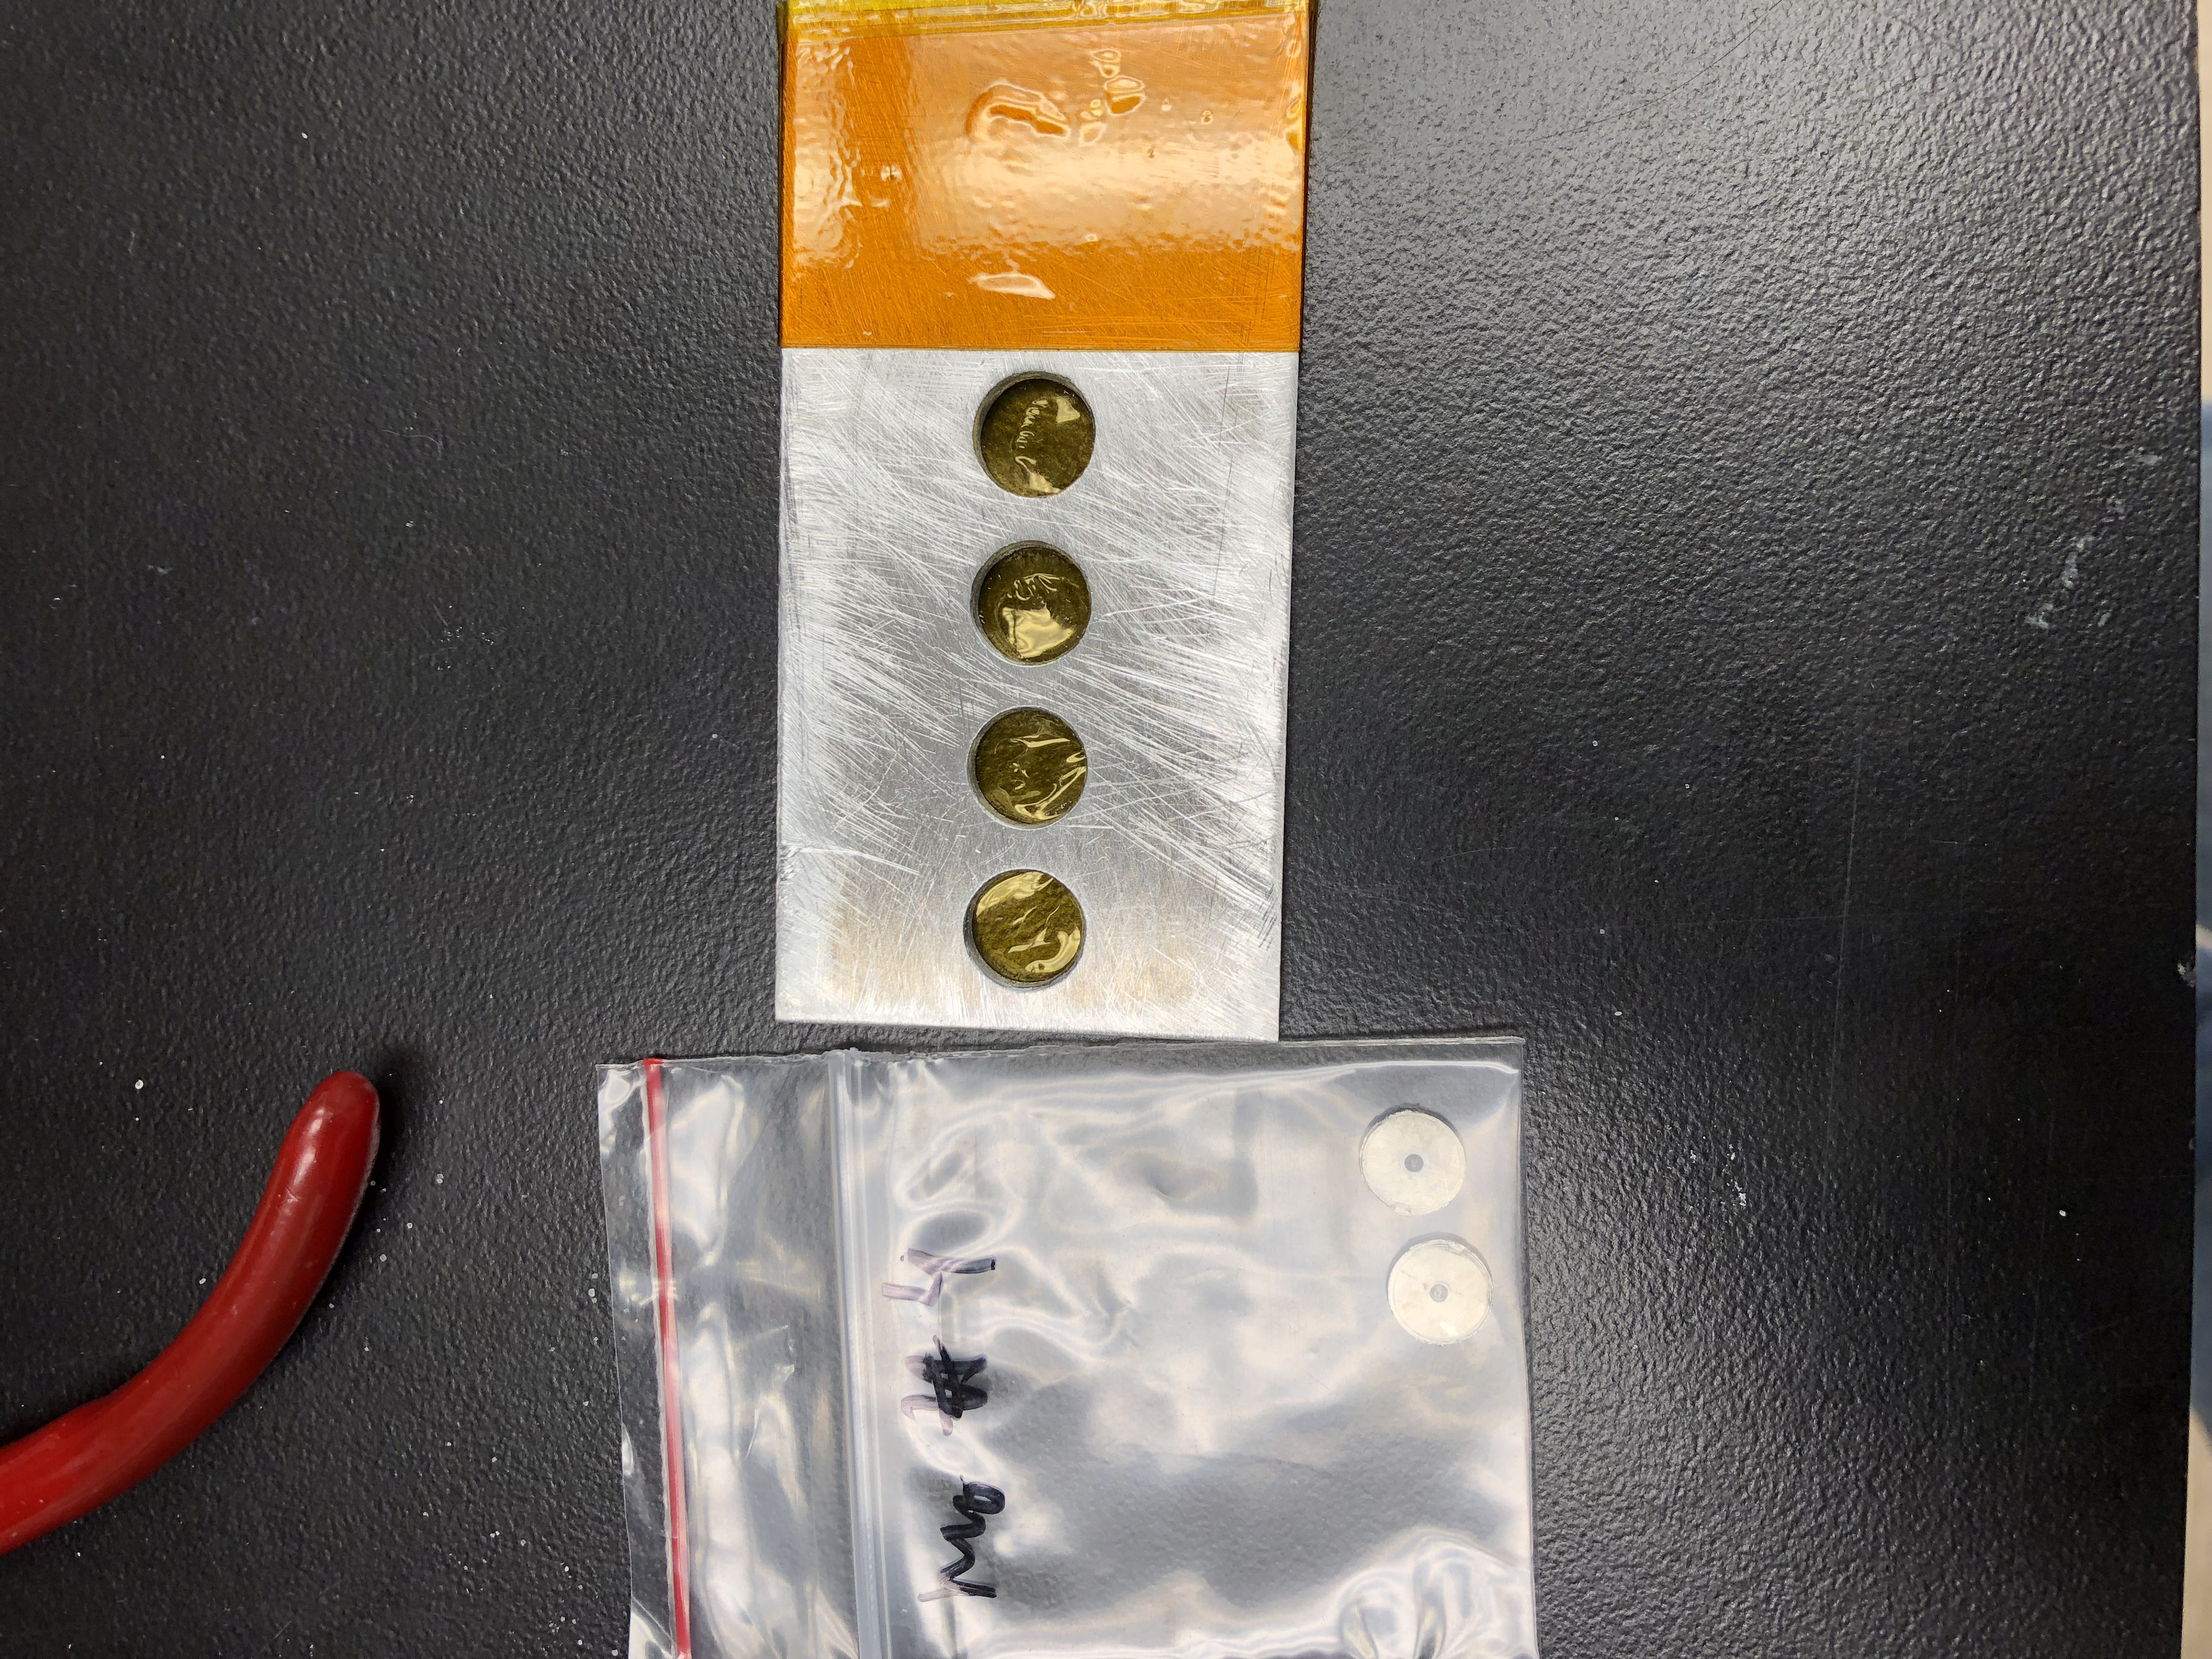
\includegraphics[clip=true,trim=5pt 1000pt 10pt 900pt,width=0.75\columnwidth,angle=90]{./figures/IMG_8840.JPG}
%  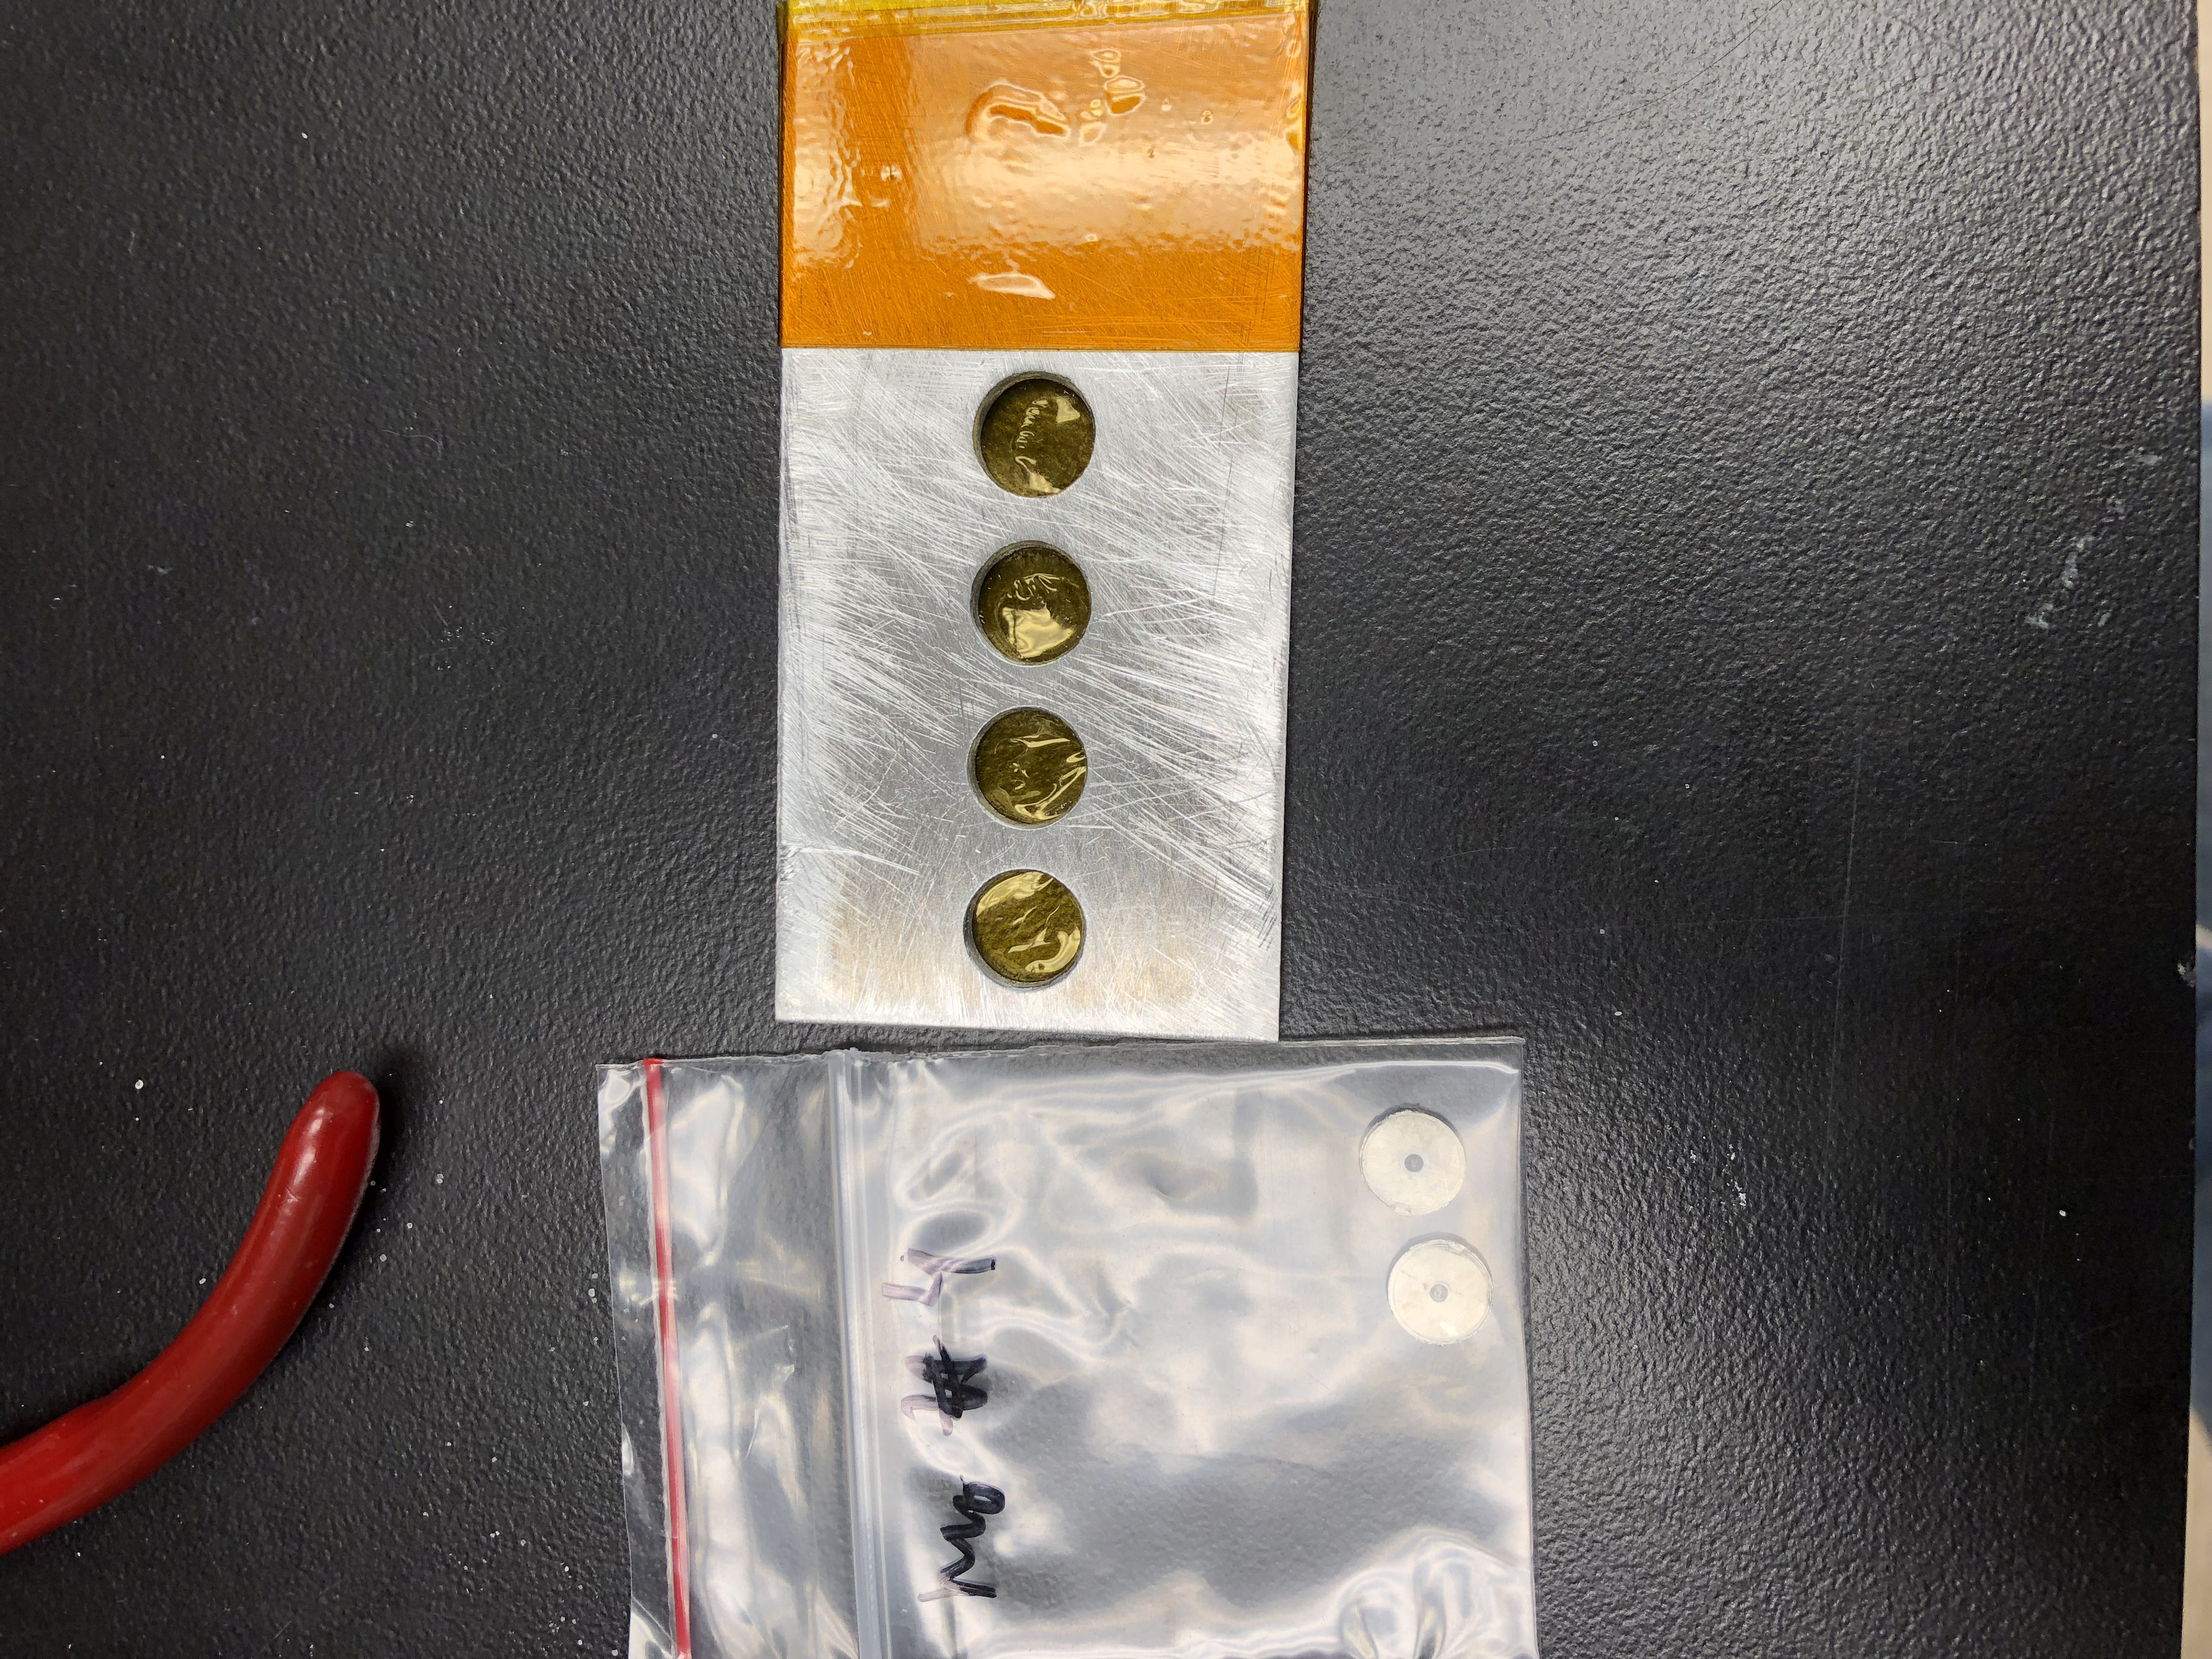
\includegraphics[width=0.75\columnwidth,angle=270]{./figures/IMG_8840.JPG}
%  \includegraphics[width=0.95\columnwidth]{./figures/Control Room Map.pdf}
 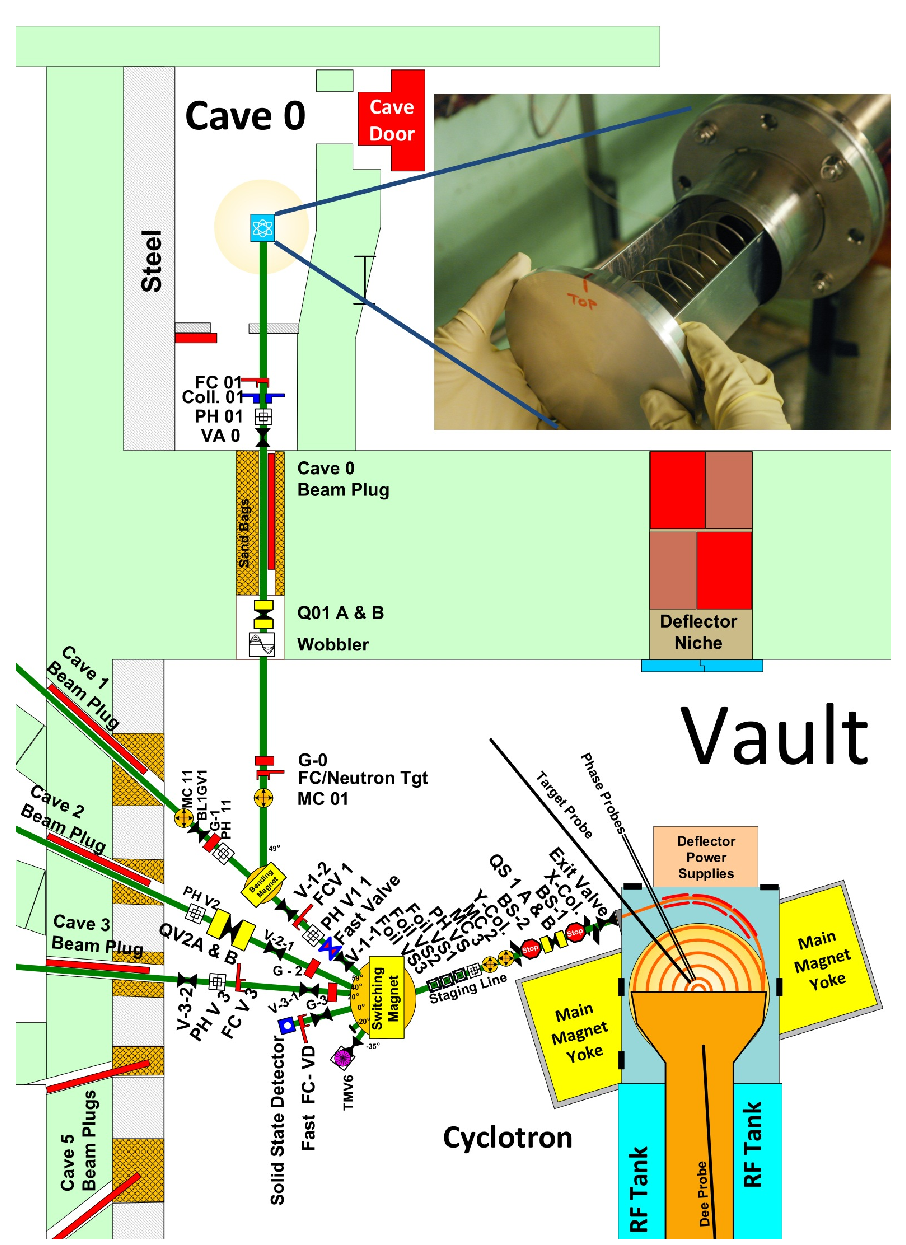
\includegraphics[height=0.90\textheight]{./figures/88beampath-cropped.pdf}
%  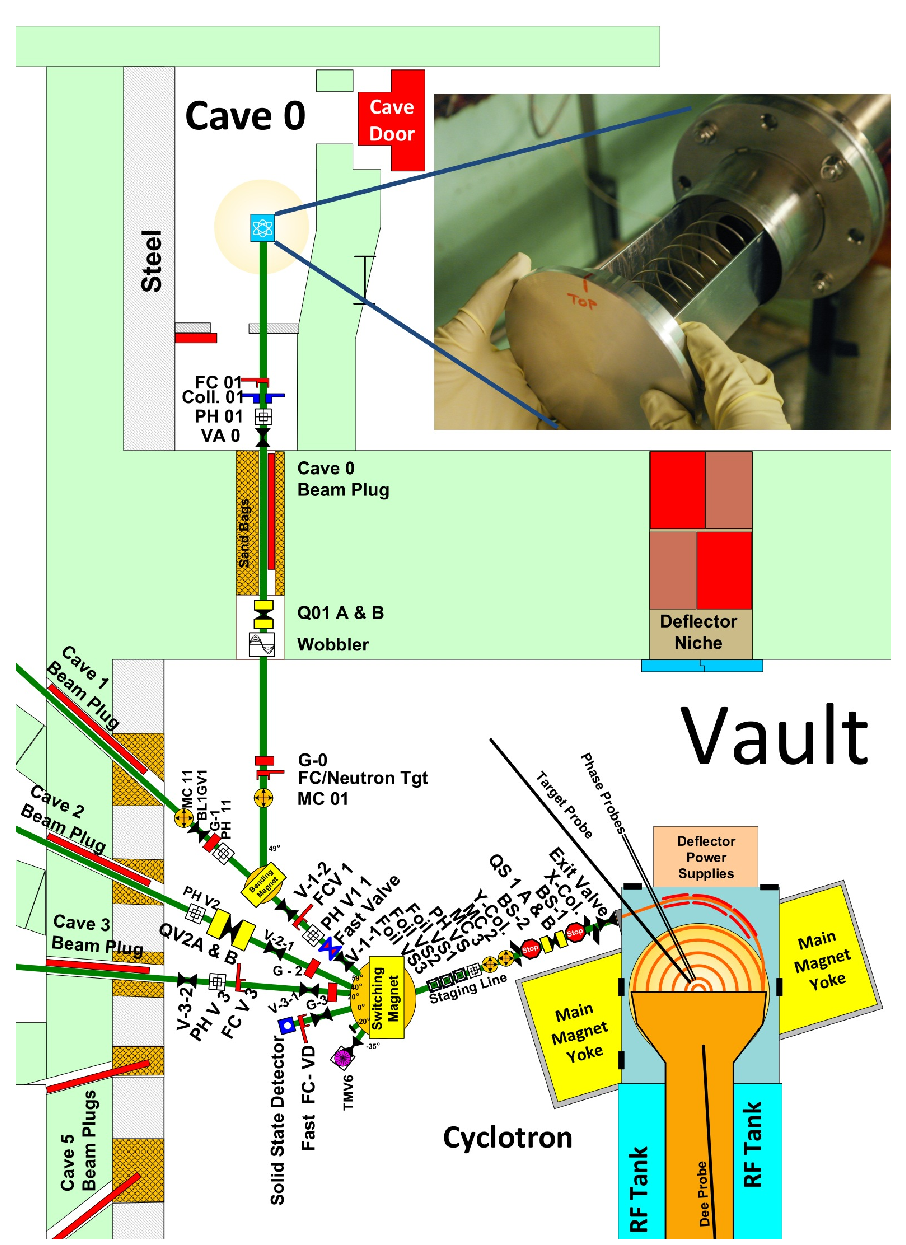
\includegraphics[width=0.95\columnwidth]{./figures/88beampath-cropped.pdf}
 % IMG_8840.JPG: 4032x3024 pixel, 72dpi, 142.24x106.68 cm, bb=0 0 4032 3024
 \caption{Schematic diagram of the 88-Inch Cyclotron facility and beamlines at LBNL, highlighting the beam path to Cave 0.  A rear view of the target stack holder used in this work is seen here, where it mounts onto the end of the Cave 0 beamline. }
 \label{fig:fe_beamline_schematic}
\end{figure}

% \begin{figure}
%  \centering
% %                                l   b      r    top
% %  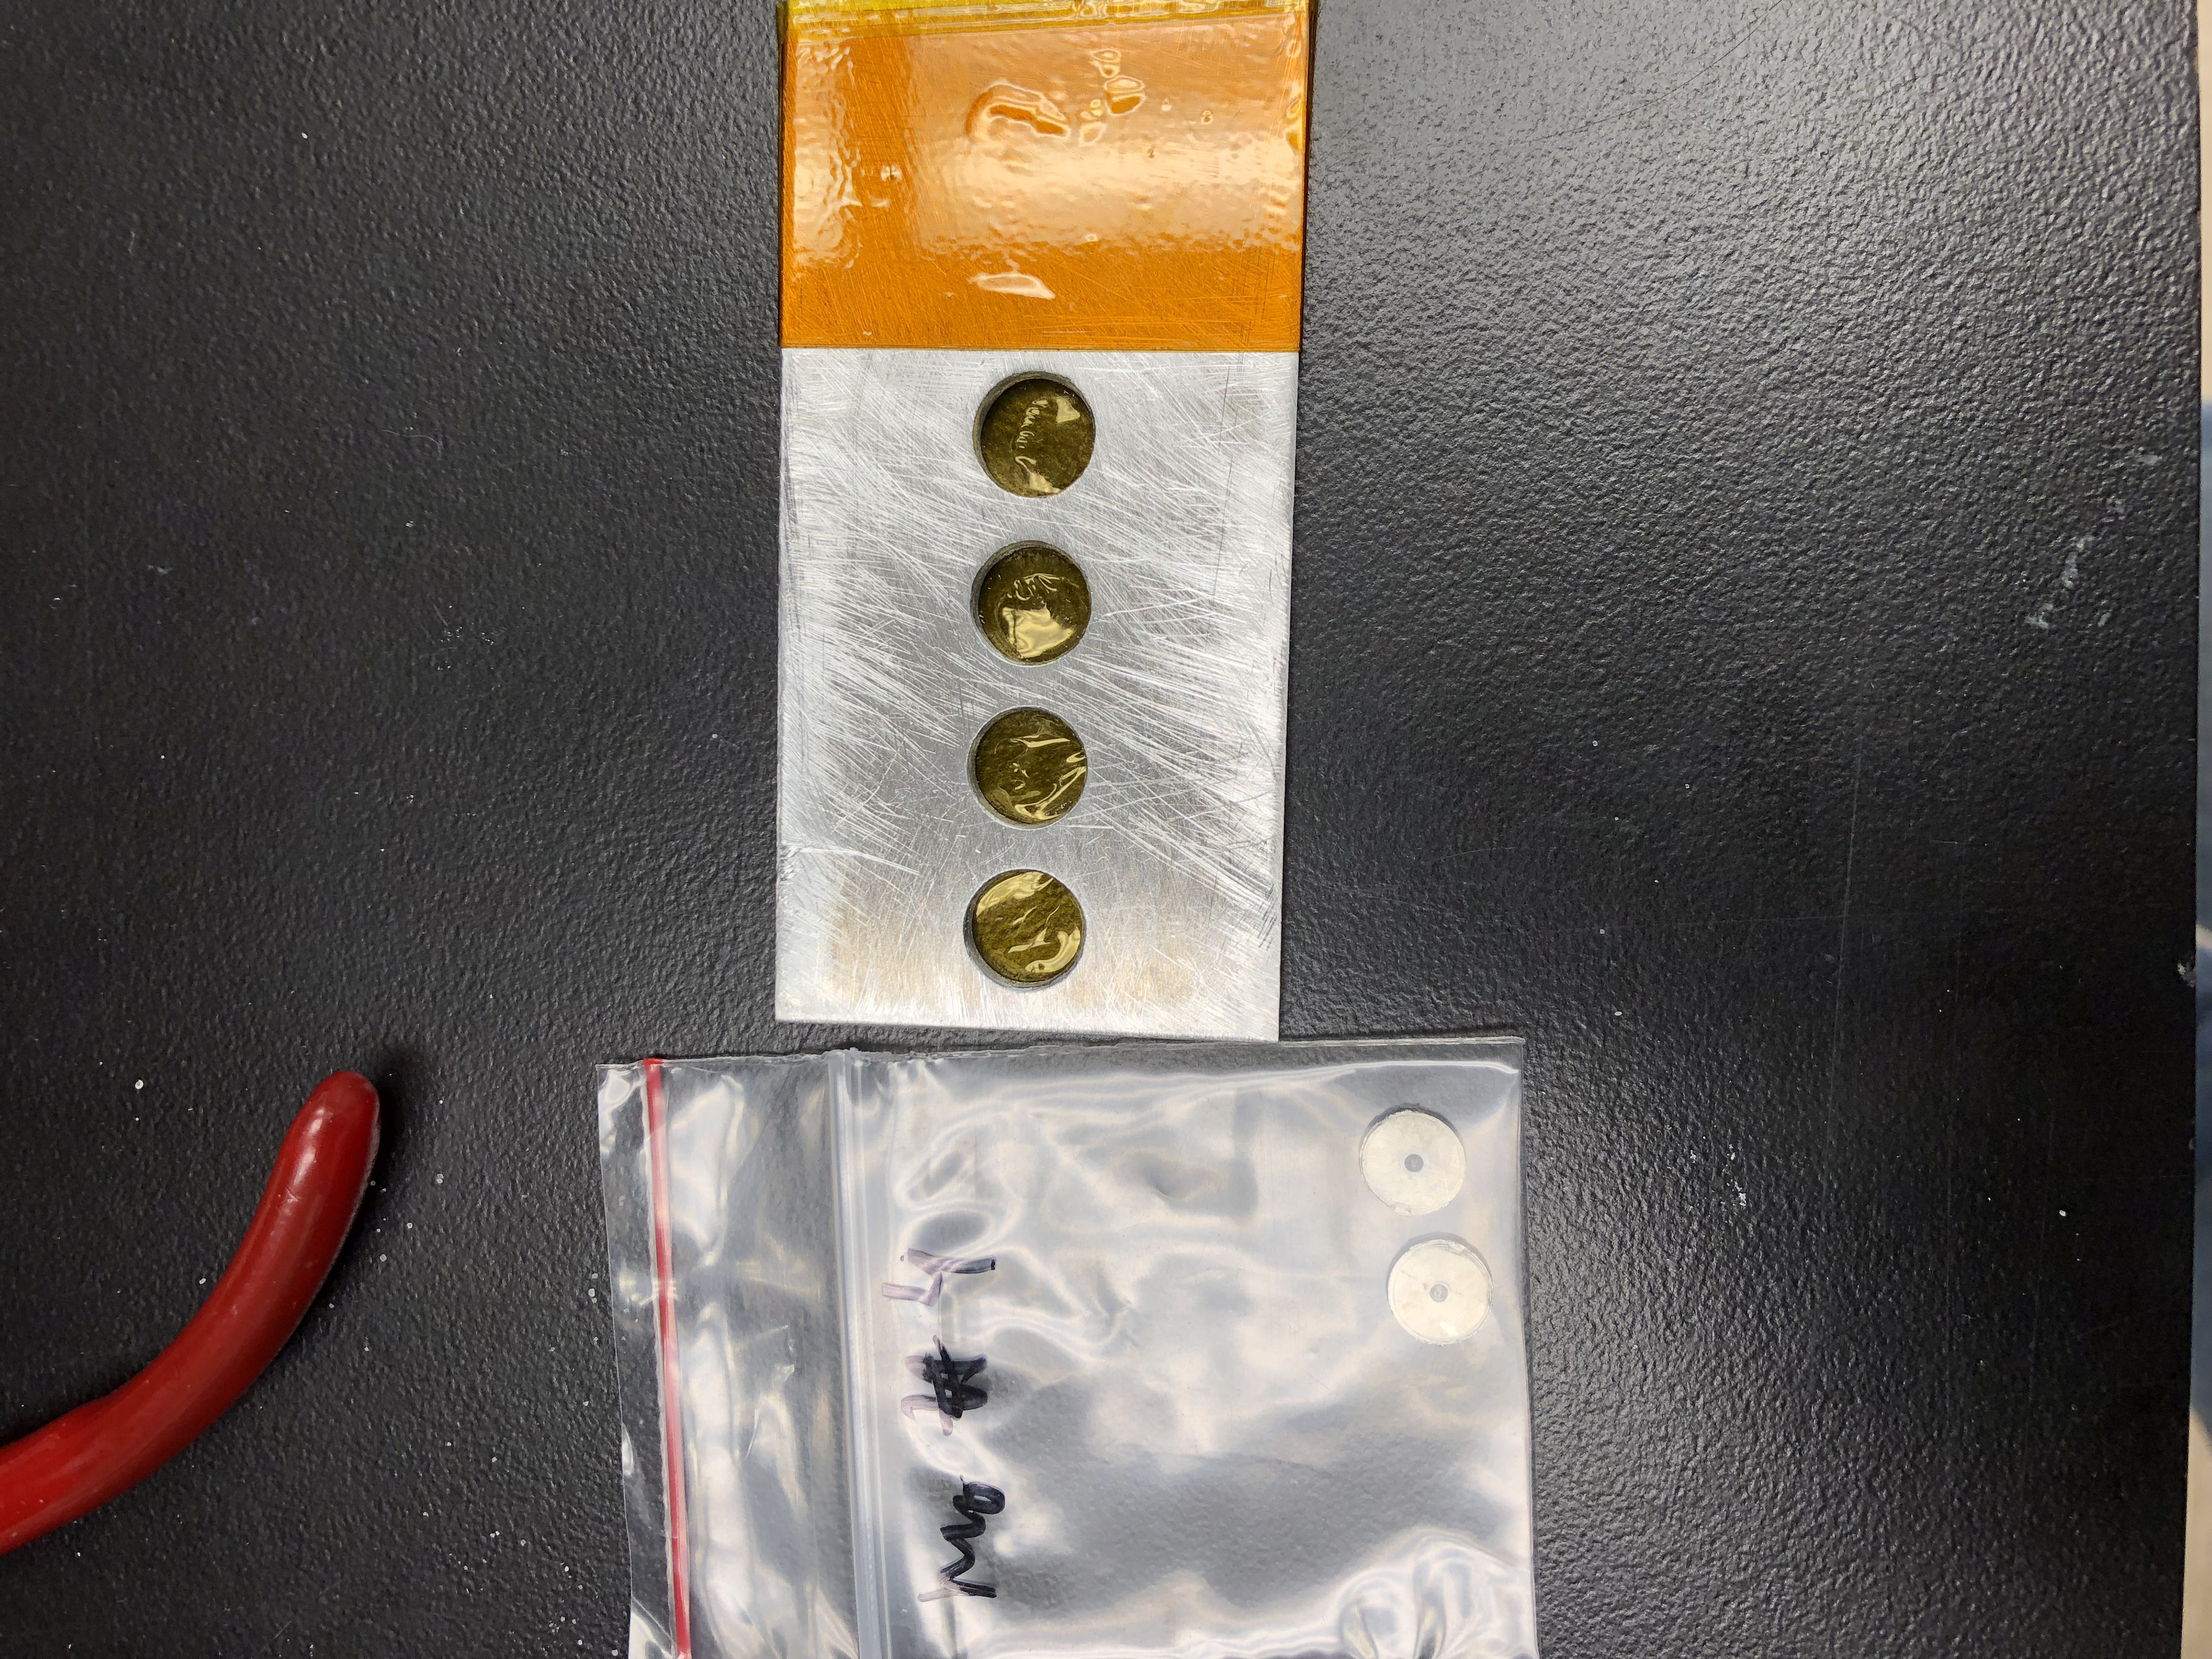
\includegraphics[clip=true,trim=5pt 1000pt 10pt 900pt,width=0.75\columnwidth,angle=90]{./figures/IMG_8840.JPG}
% %  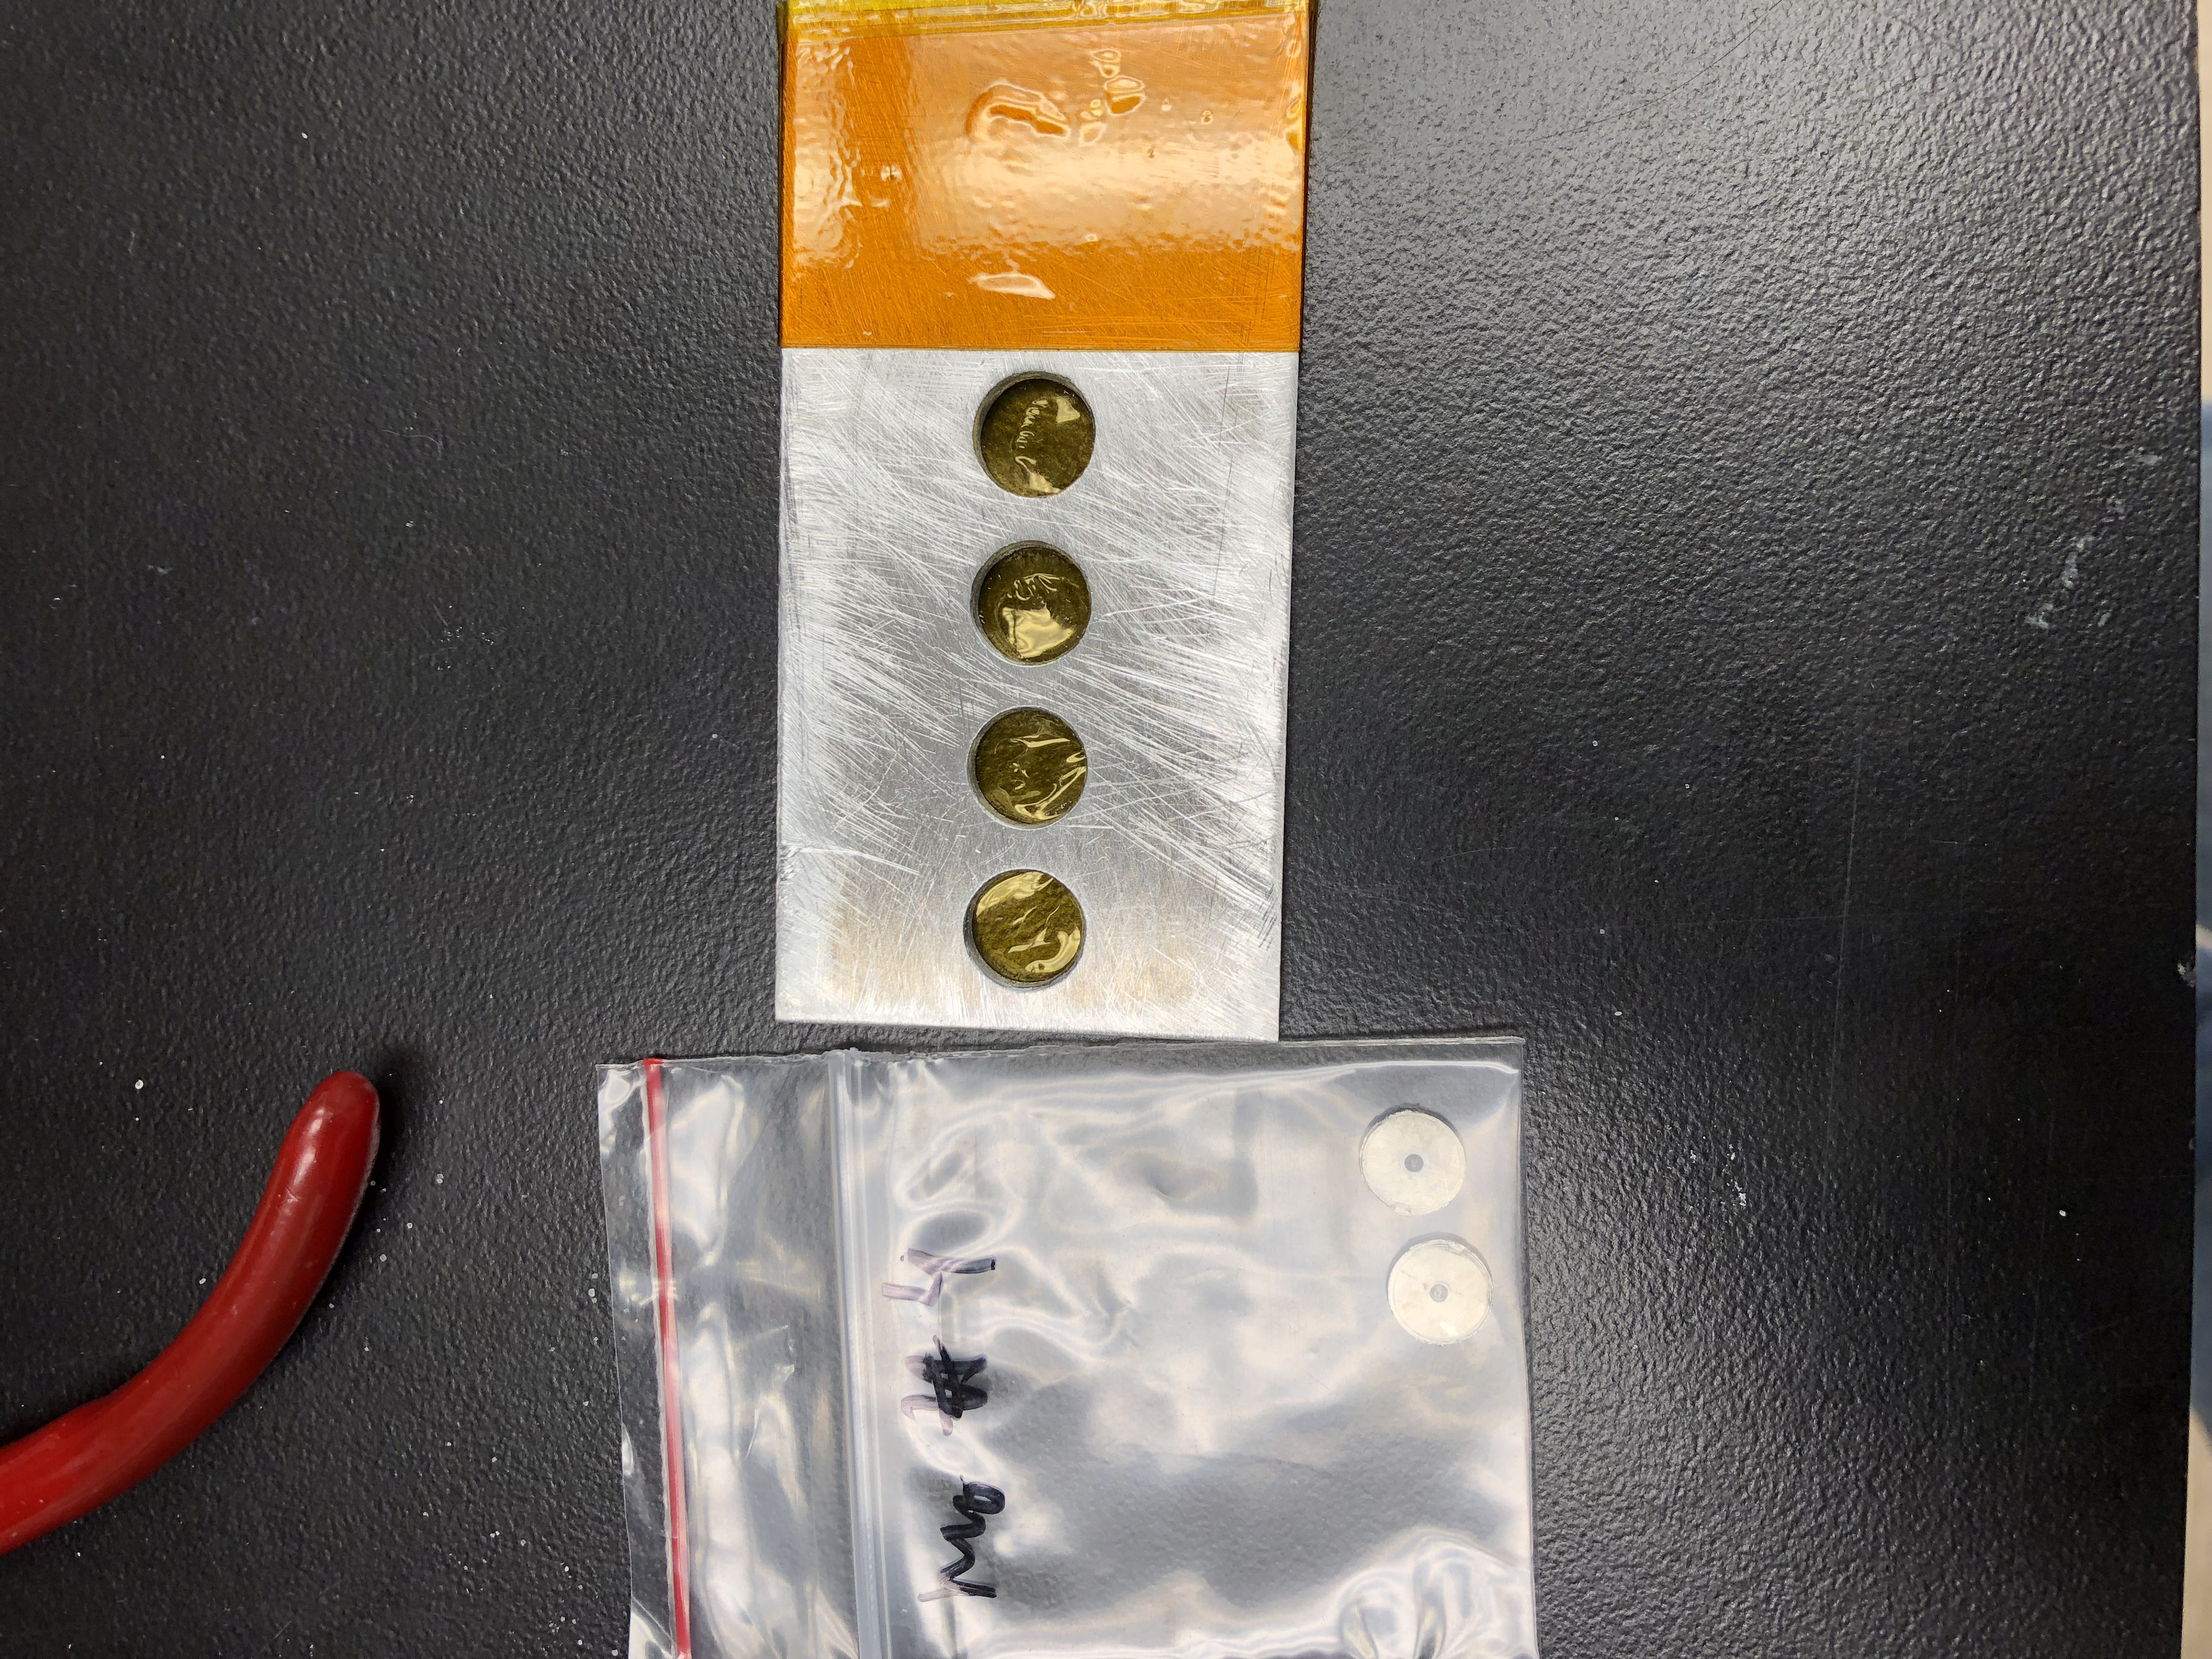
\includegraphics[width=0.75\columnwidth,angle=270]{./figures/IMG_8840.JPG}
%  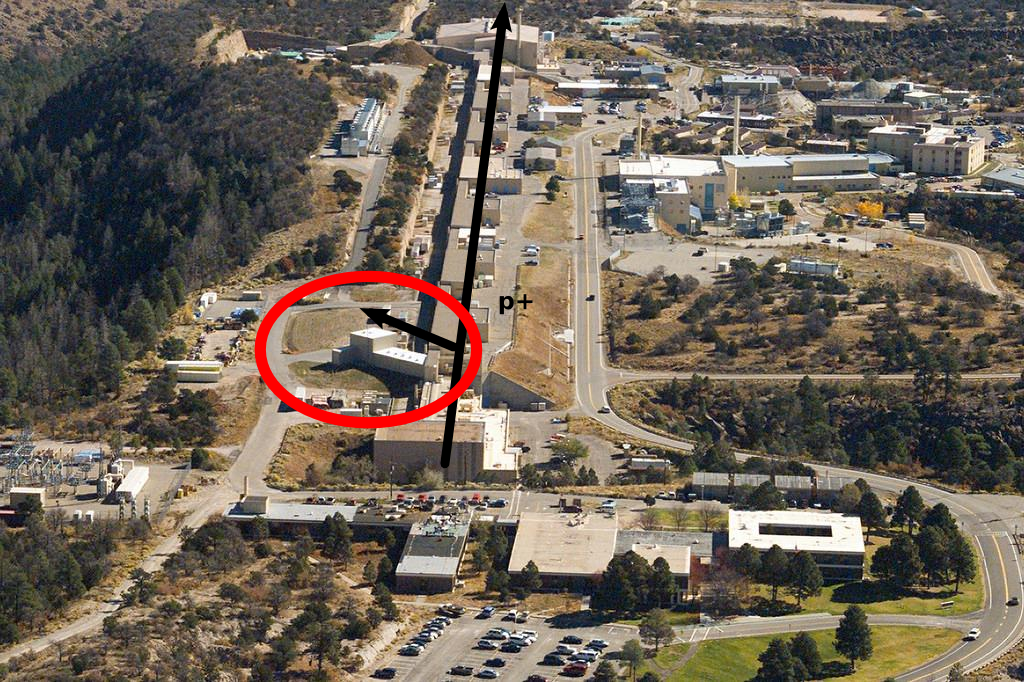
\includegraphics[width=0.75\columnwidth]{./figures/ipf_beamline_alternate.png}
%  % IMG_8840.JPG: 4032x3024 pixel, 72dpi, 142.24x106.68 cm, bb=0 0 4032 3024
%  \caption{Aerial photograph of the LANSCE beamline. Proton injectors are seen in the foreground building near the arrow's tail. The IPF beamline and operations facility is seen to the left of the main LANSCE beamline, circled in red.  The target box seen in \autoref{fig:target_stack} is lowered into the beamline here, via a hot cell.}
%  \label{fig:fe_beamline_alternate}
% \end{figure}





\subsubsection{Beam profile measurements}




% Following  tuning of the 25 and 55\,MeV proton beams into Cave 0, the  final remaining step prior to loading the  target box for irradiation is to tune the beam optics and spatial profile.
% In the prior fielding run from April 2016, this was performed by loading 3 pieces of the EBT3 Gafchromic film (the same as used for imaging the beam  with stainless steel profile monitors) into the empty target stack holder, with one at the front end, one at the rear, and one in the middle.
% At this point, the target stack would be mounted into the beamline, which would be pumped down to the 
% 40\,$\mmicro$torr
% beamline pressure for a run.
% Following pumpdown, the \enquote{stack} of films would be exposed to an extremely short, low-current pulse of the tuned proton beam (approximately 0.1\,nAh for 1\,s), to directly expose the films and image the beam profile and optics.
% Running any more beam fluence than this would cause the entire film to be massively overexposed, nullifying its usefulness.
% At this point, the beamline would be brought up to atmosphere, and  the films removed for interpretation.
% The cyclotron operator would then use the films to adjust the beam's horizontal and vertical position, and tune the beam optics to produce a \enquote{pencil-beam} spatial profile.
% This is to ensure that the beam spot will be centered on the mounted target foils, and fully constrained within the foils, under-filling them.
% After tuning the beam's optics, more films would be loaded, and this process would be repeated multiple times, confirming any adjustments made to improve the optics, until an acceptable beam spot was achieved. 
% Each cycle of loading and unloading a set of films would take approximately 45\,min, followed by approximately another 30\,min to make any beam adjustments, followed by the 1\,s film exposure.
% As a result, during this fielding run, optical tuning took nearly an entire day of beam time, which would be infeasible for future experiments.


% To improve this process, 
In order to expedite the tuning process, I designed a phosphor target to mount into the end of the beamline during final optics tuning.
% , sealing onto the beamline during pumpdown via an inset o-ring.
The design was based off of designs for the beam stop component of the target stack holder, but instead of featuring a solid aluminum end cap, it has a circular opening, designed to hold a glass puck.
This puck forms a vacuum seal through an inset o-ring, and is held against the rear of the target by an aluminum frame.
The blueprints for this phosphor are seen in \autoref{fig:fe_phosphor}.
On the inside (beamline-facing) side of the glass puck, a thin layer of vacuum grease was painted on, and mixed with a powdered phosphorescent paint, to create a thin phosphorescent layer.
This target is mounted onto the end of the beamline during optics tuning, and has been used in all experiments since.
When exposed to a low-current (approximately 0.1\,nA) beam, the phosphor glows brightly, outlining the beam profile.
A low current is used, to ensure that the phosphor layer does not get overly heated and burn or flake off during tuning.
By patching in a camera to the cave, the operators may tune the beam optics in real time, moving the beam spot and improving its spatial profile, while watching on a video feed from the remote camera.
This has drastically shortened the optics tuning process from 6--8\,hours down to less than a single hour, and has made all subsequent experiments far easier in the process.
A remote view of this phosphor target during tuning is seen in \autoref{fig:fe_preexp_beam_spot}.



\begin{figure}
    \centering
    \subfloat{
        \centering
%         \includegraphics[width=\columnwidth]{./figures/Capture.PNG}
        \hspace{-1pt}\subfigimg[width=0.925\textwidth]{a)}{./figures/Phosphor_Cap_Blueprints.pdf}{50}
%         \caption{ Decay curve for the isomeric transition of \ce{^{115m}In}.}
         %         \refstepcounter{subfigure}
%          \label{fig:fe_before_minimization}
   \hspace{-5pt}}%
     \subfloat{
        \centering
\\
%         \subfigimg[width=0.5\textwidth]{b)}{./figures/after_minimization_plot.pdf}{50}
        \subfigimg[width=0.4\textwidth]{\textcolor{white}{b)}}{./figures/perspective.png}{50}
         %         \refstepcounter{subfigure}
%          \label{fig:fe_after_minimization}
   \hspace{-5pt}}%
    \caption{Blueprints (a) and 3D cutaway rendering (b) of the phosphor target used for real-time beam optics tuning at the 88-Inch Cyclotron.} 
%     Following minimization, additional apparent fluence is observed in the  \ce{^{nat}Al}(p,x)\ce{^{22}Na} and \ce{^{nat}Al}(p,x)\ce{^{24}Na} monitor channels, due to contamination from \ce{^{nat}Si}(p,x)\ce{^{22,24}Na} on the silicone adhesive used for sealing foil packets.}
     \label{fig:fe_phosphor}
\end{figure}


However, this phosphor target offers a fairly low-resolution image of the beam profile, mostly useful as a qualitative guide for tuning.
As a result, a final film exposure is performed after beam optics appear satisfactory on the phosphor, to confirm the optics tune.
After verifying that 
% loading a sheet of polyethylene (approximately 3\,mm thick) into the the IPF beamline, at the same location of the target box's beam entrance window. 
% This sheet acts as a beam profile monitor, and is irradiated with 5 \mmicro A-min of the proton beam.
% Following exposure, the polyethylene monitor is withdrawn back into the IPF hot cell, where it is inspected to verify the shape and location of the beam profile.
% These beam profile irradiations leave an annealable discoloration of the beam profile, which resembles a \enquote{burn mark}, and are observed to passively revert within 1--2 weeks.
% The final pre-irradiation beam spot from the Nb(p.x) measurement is seen in  \autoref{fig:ipf_preexp_beam_spot}.
% LANSCE accelerator operations staff use this feedback to fine-tune the beam, 
the beam spot is centered upon the target stack and focusing it to ensure that it underfills the target foils, the foils are loaded into the stack target holder, mounted in the beamline, and the irradiation commences.
 








\begin{figure}
 \centering
%                                l   b      r    top
%  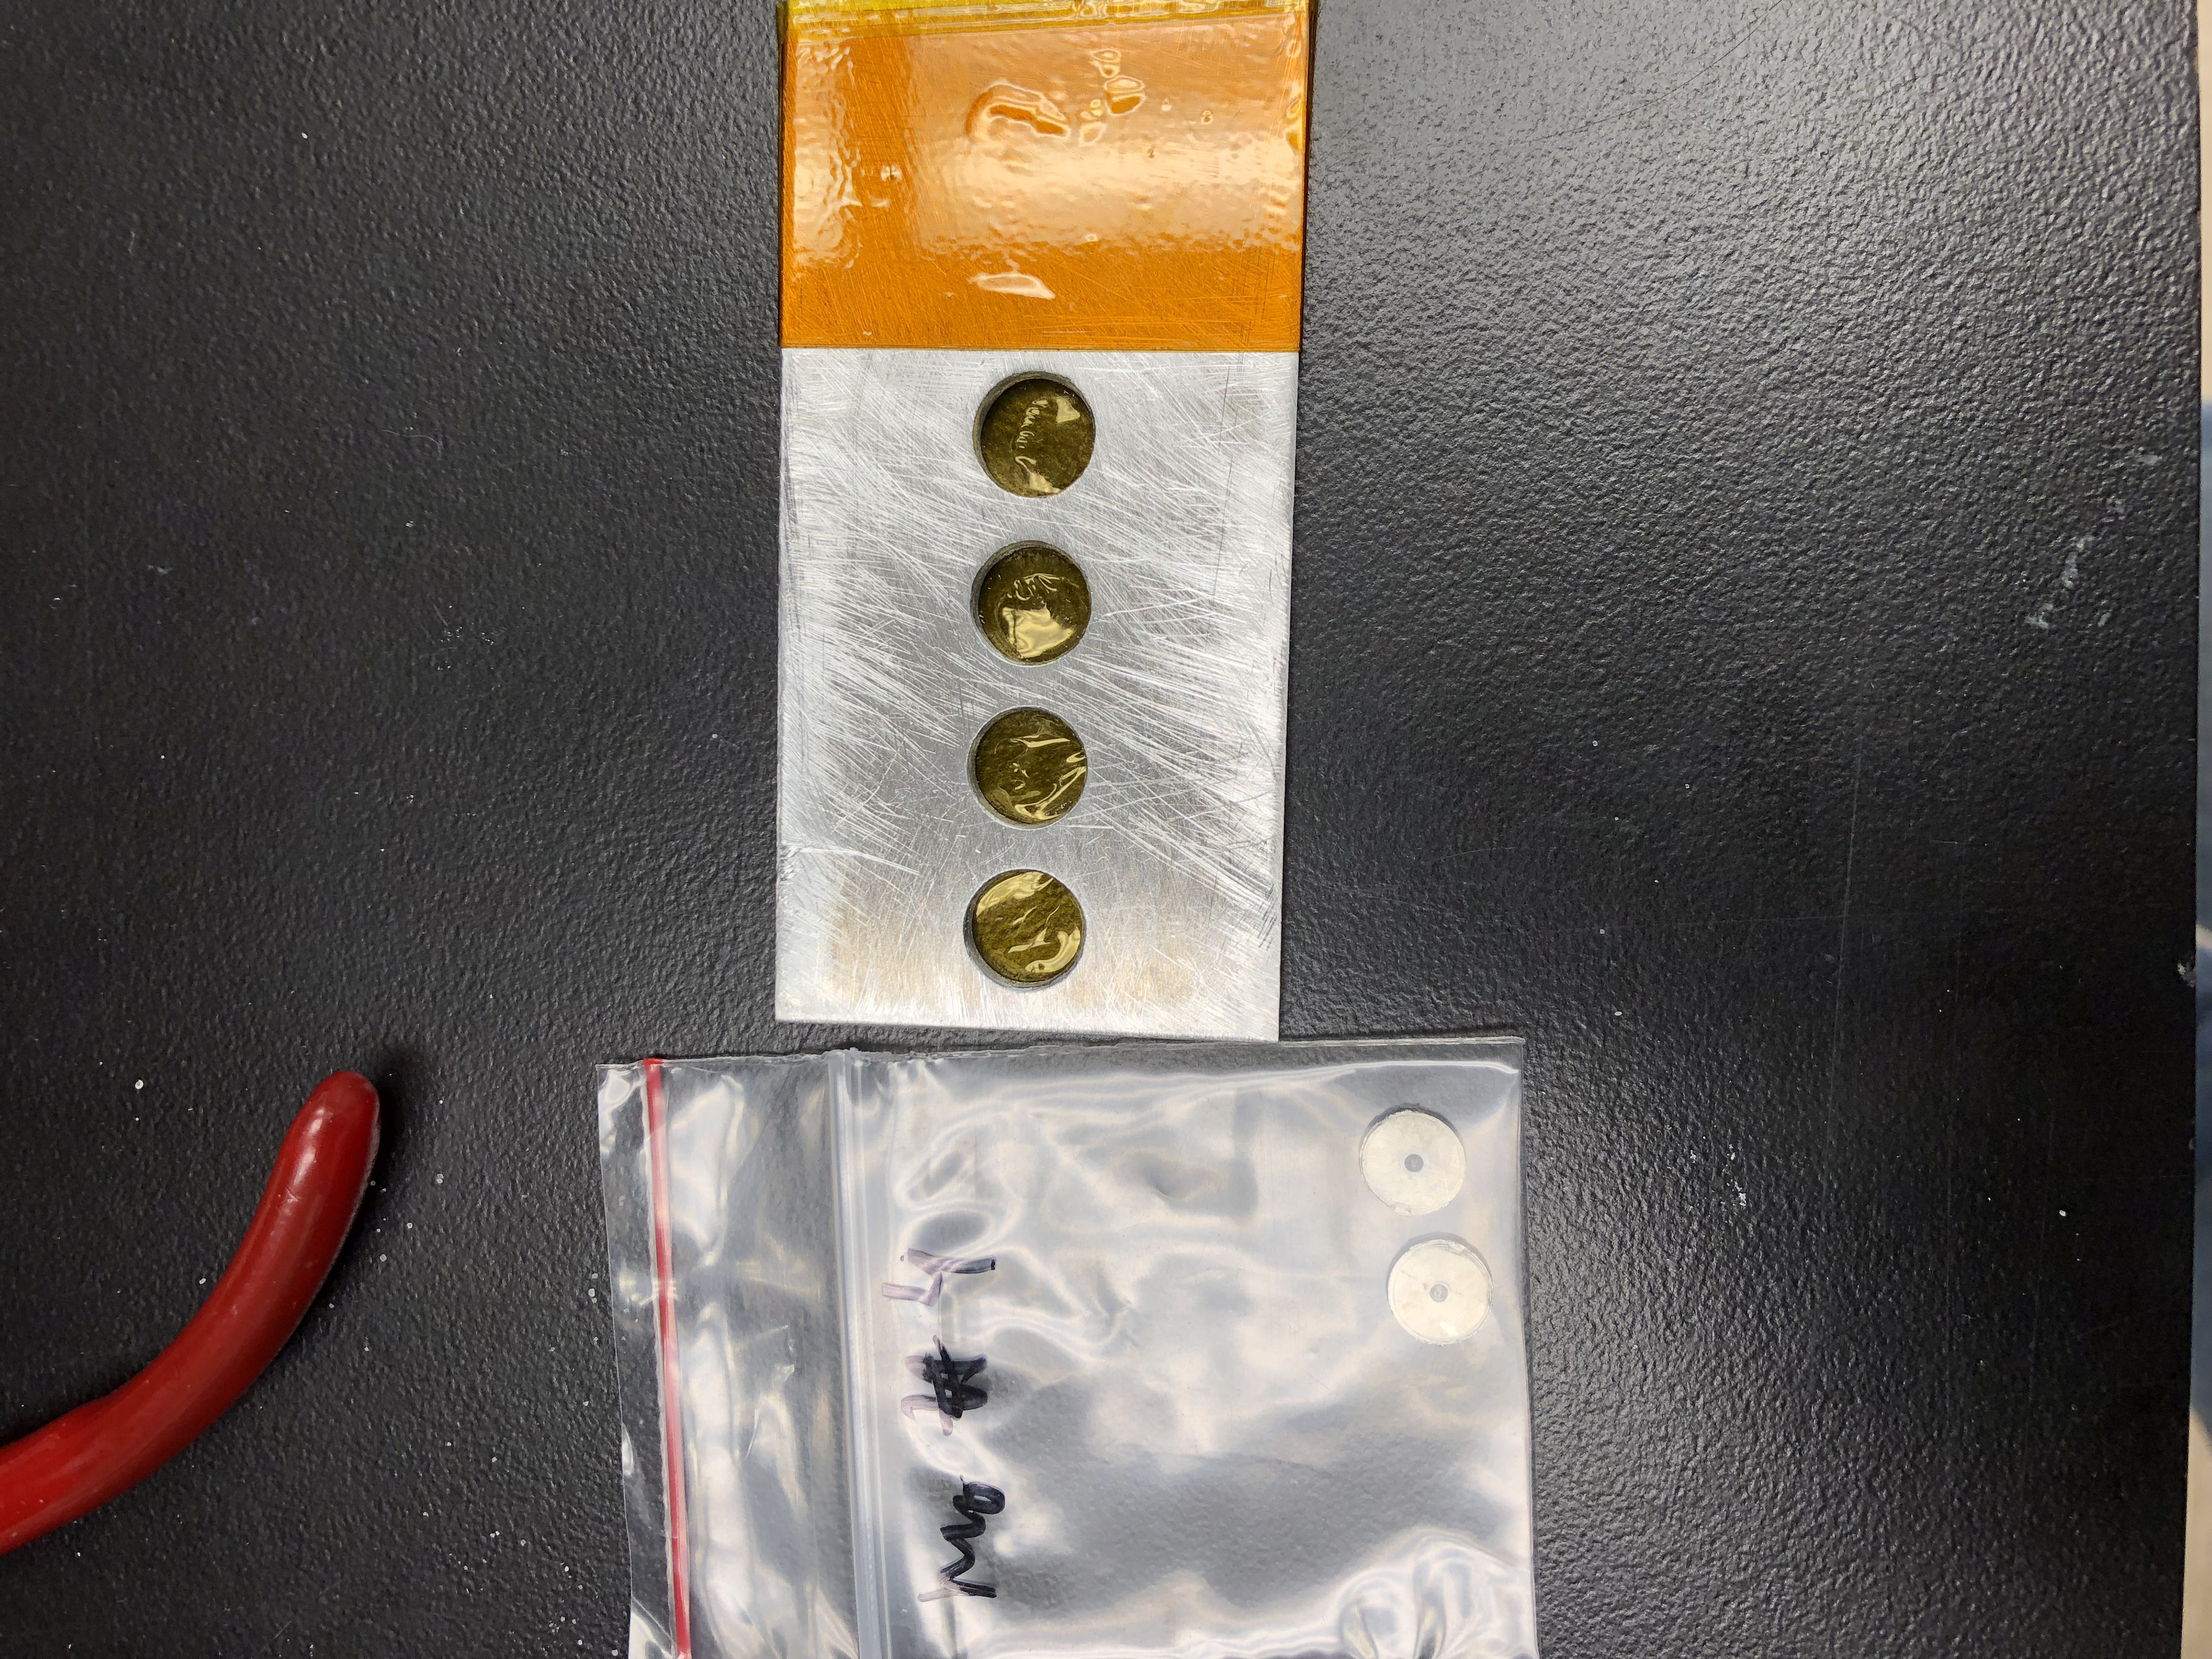
\includegraphics[clip=true,trim=5pt 1000pt 10pt 900pt,width=0.75\columnwidth,angle=90]{./figures/IMG_8840.JPG}
%  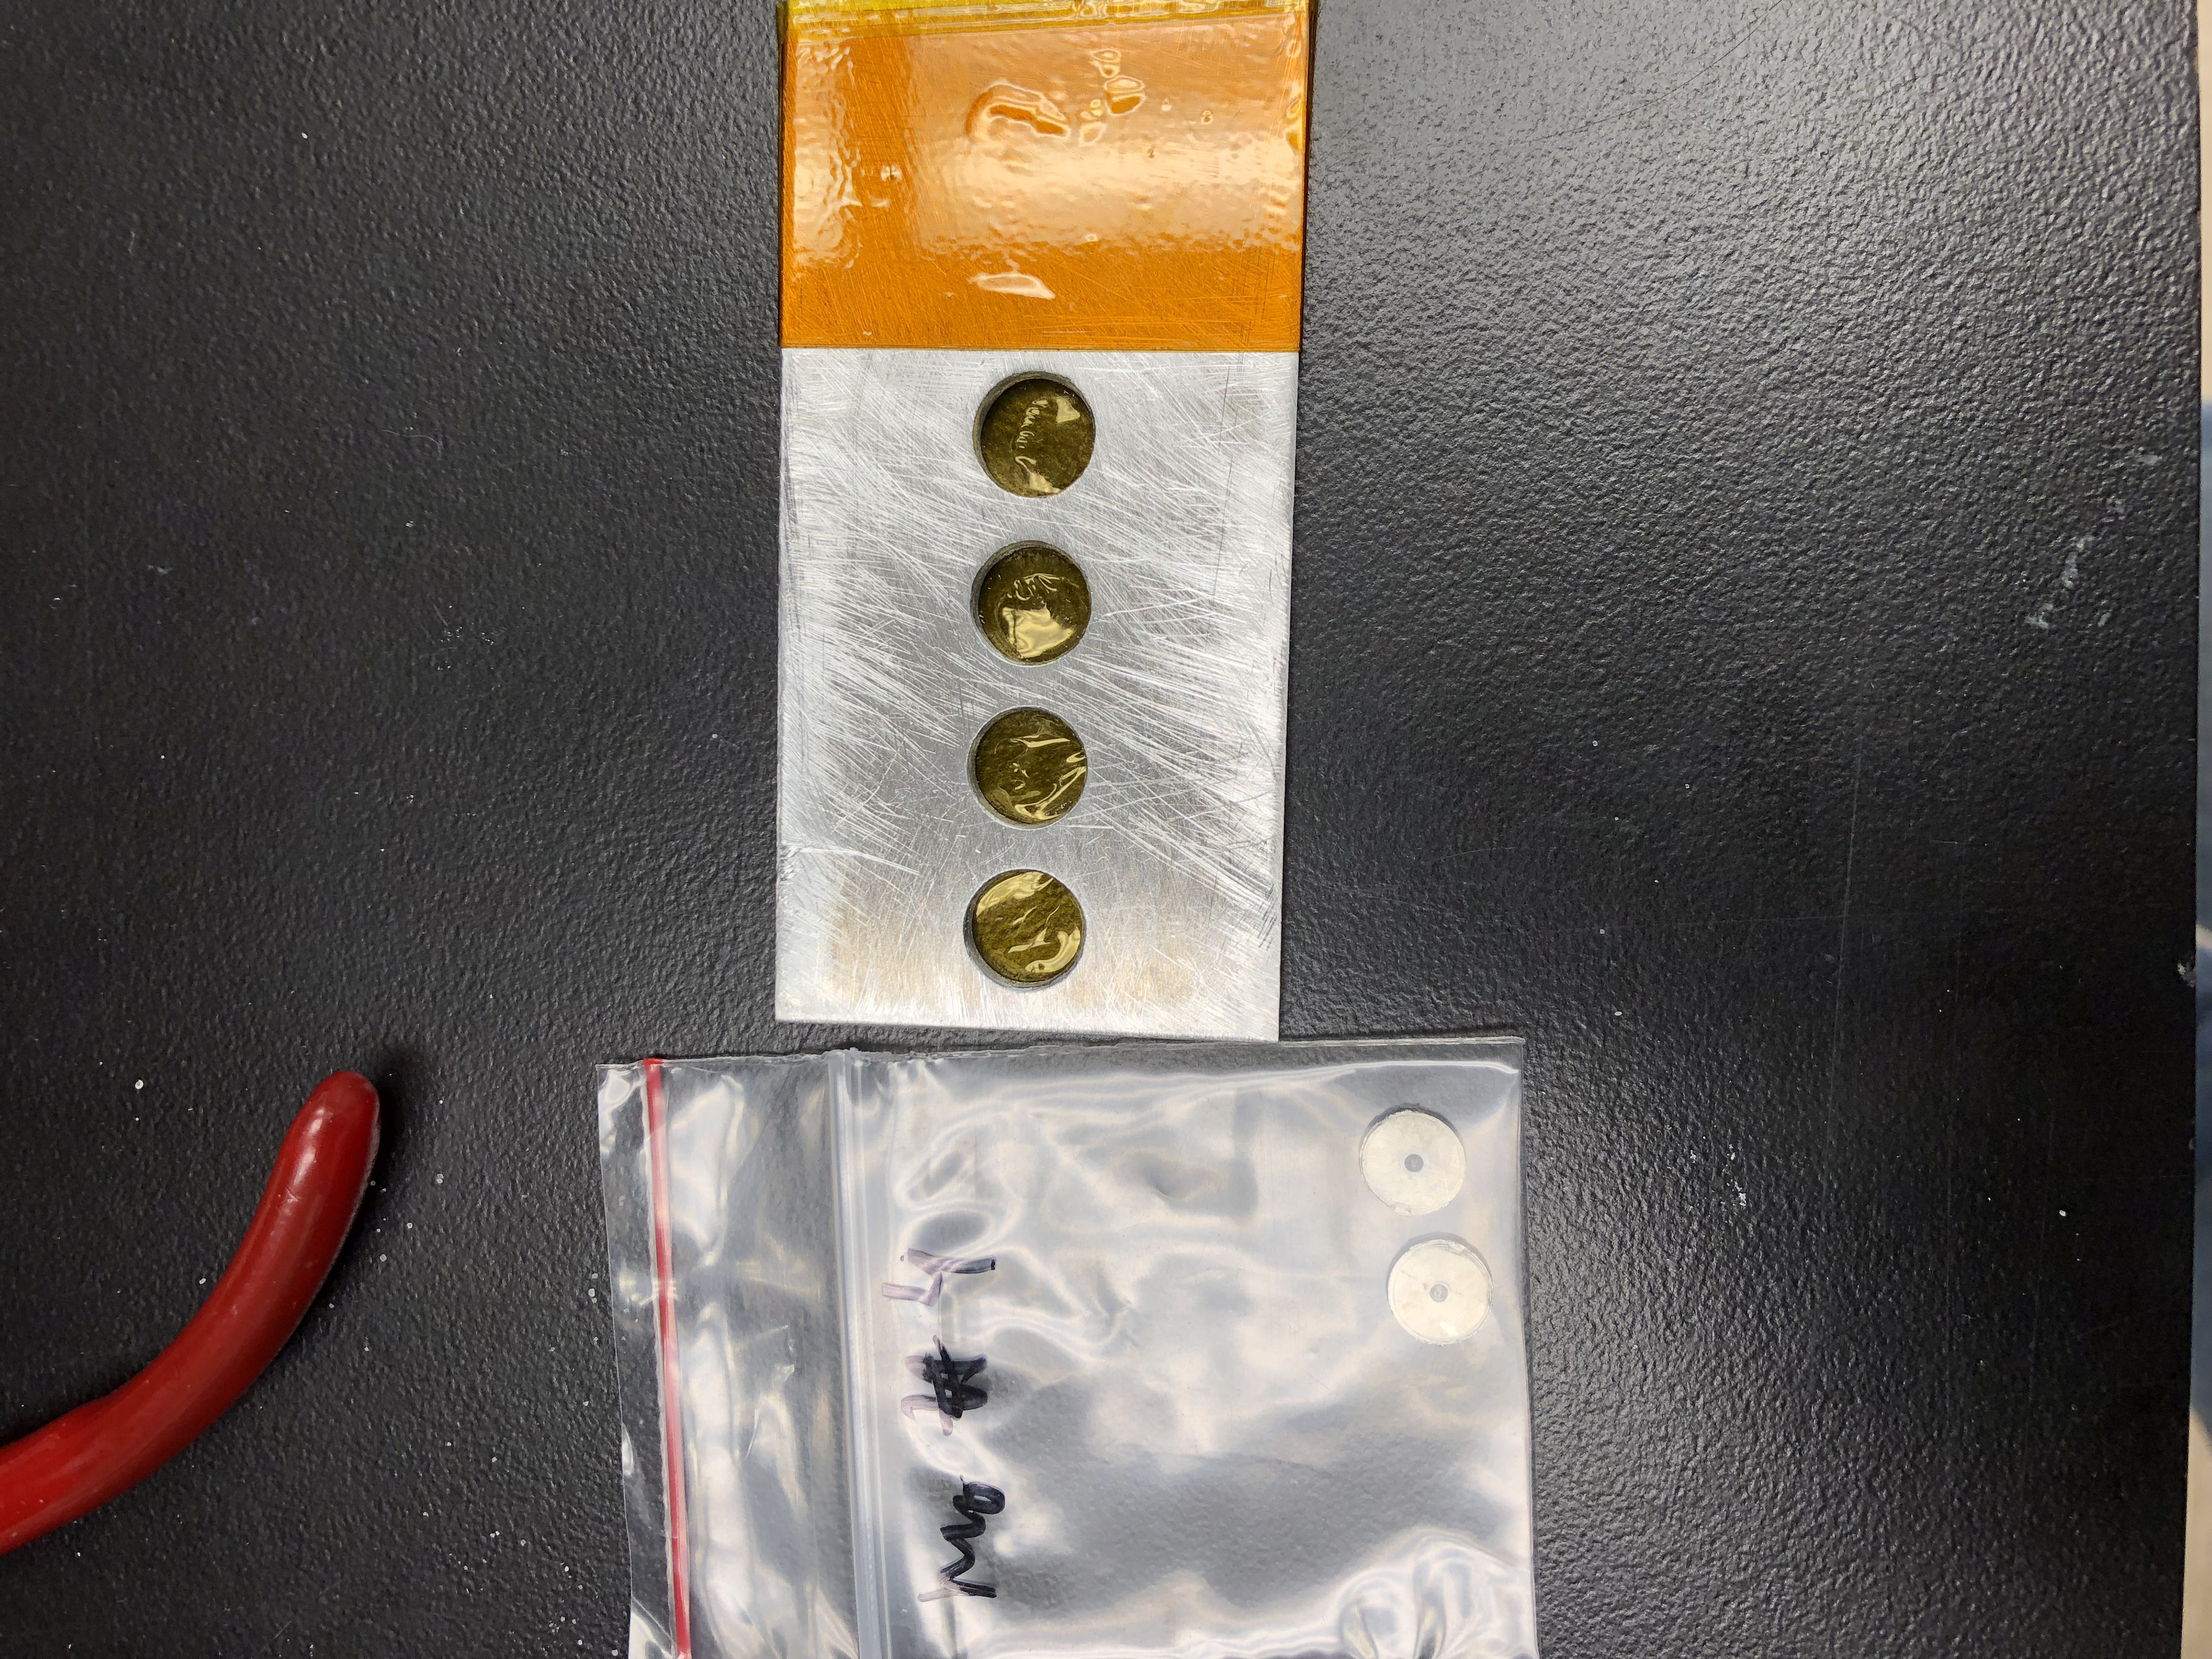
\includegraphics[width=0.75\columnwidth,angle=270]{./figures/IMG_8840.JPG}
 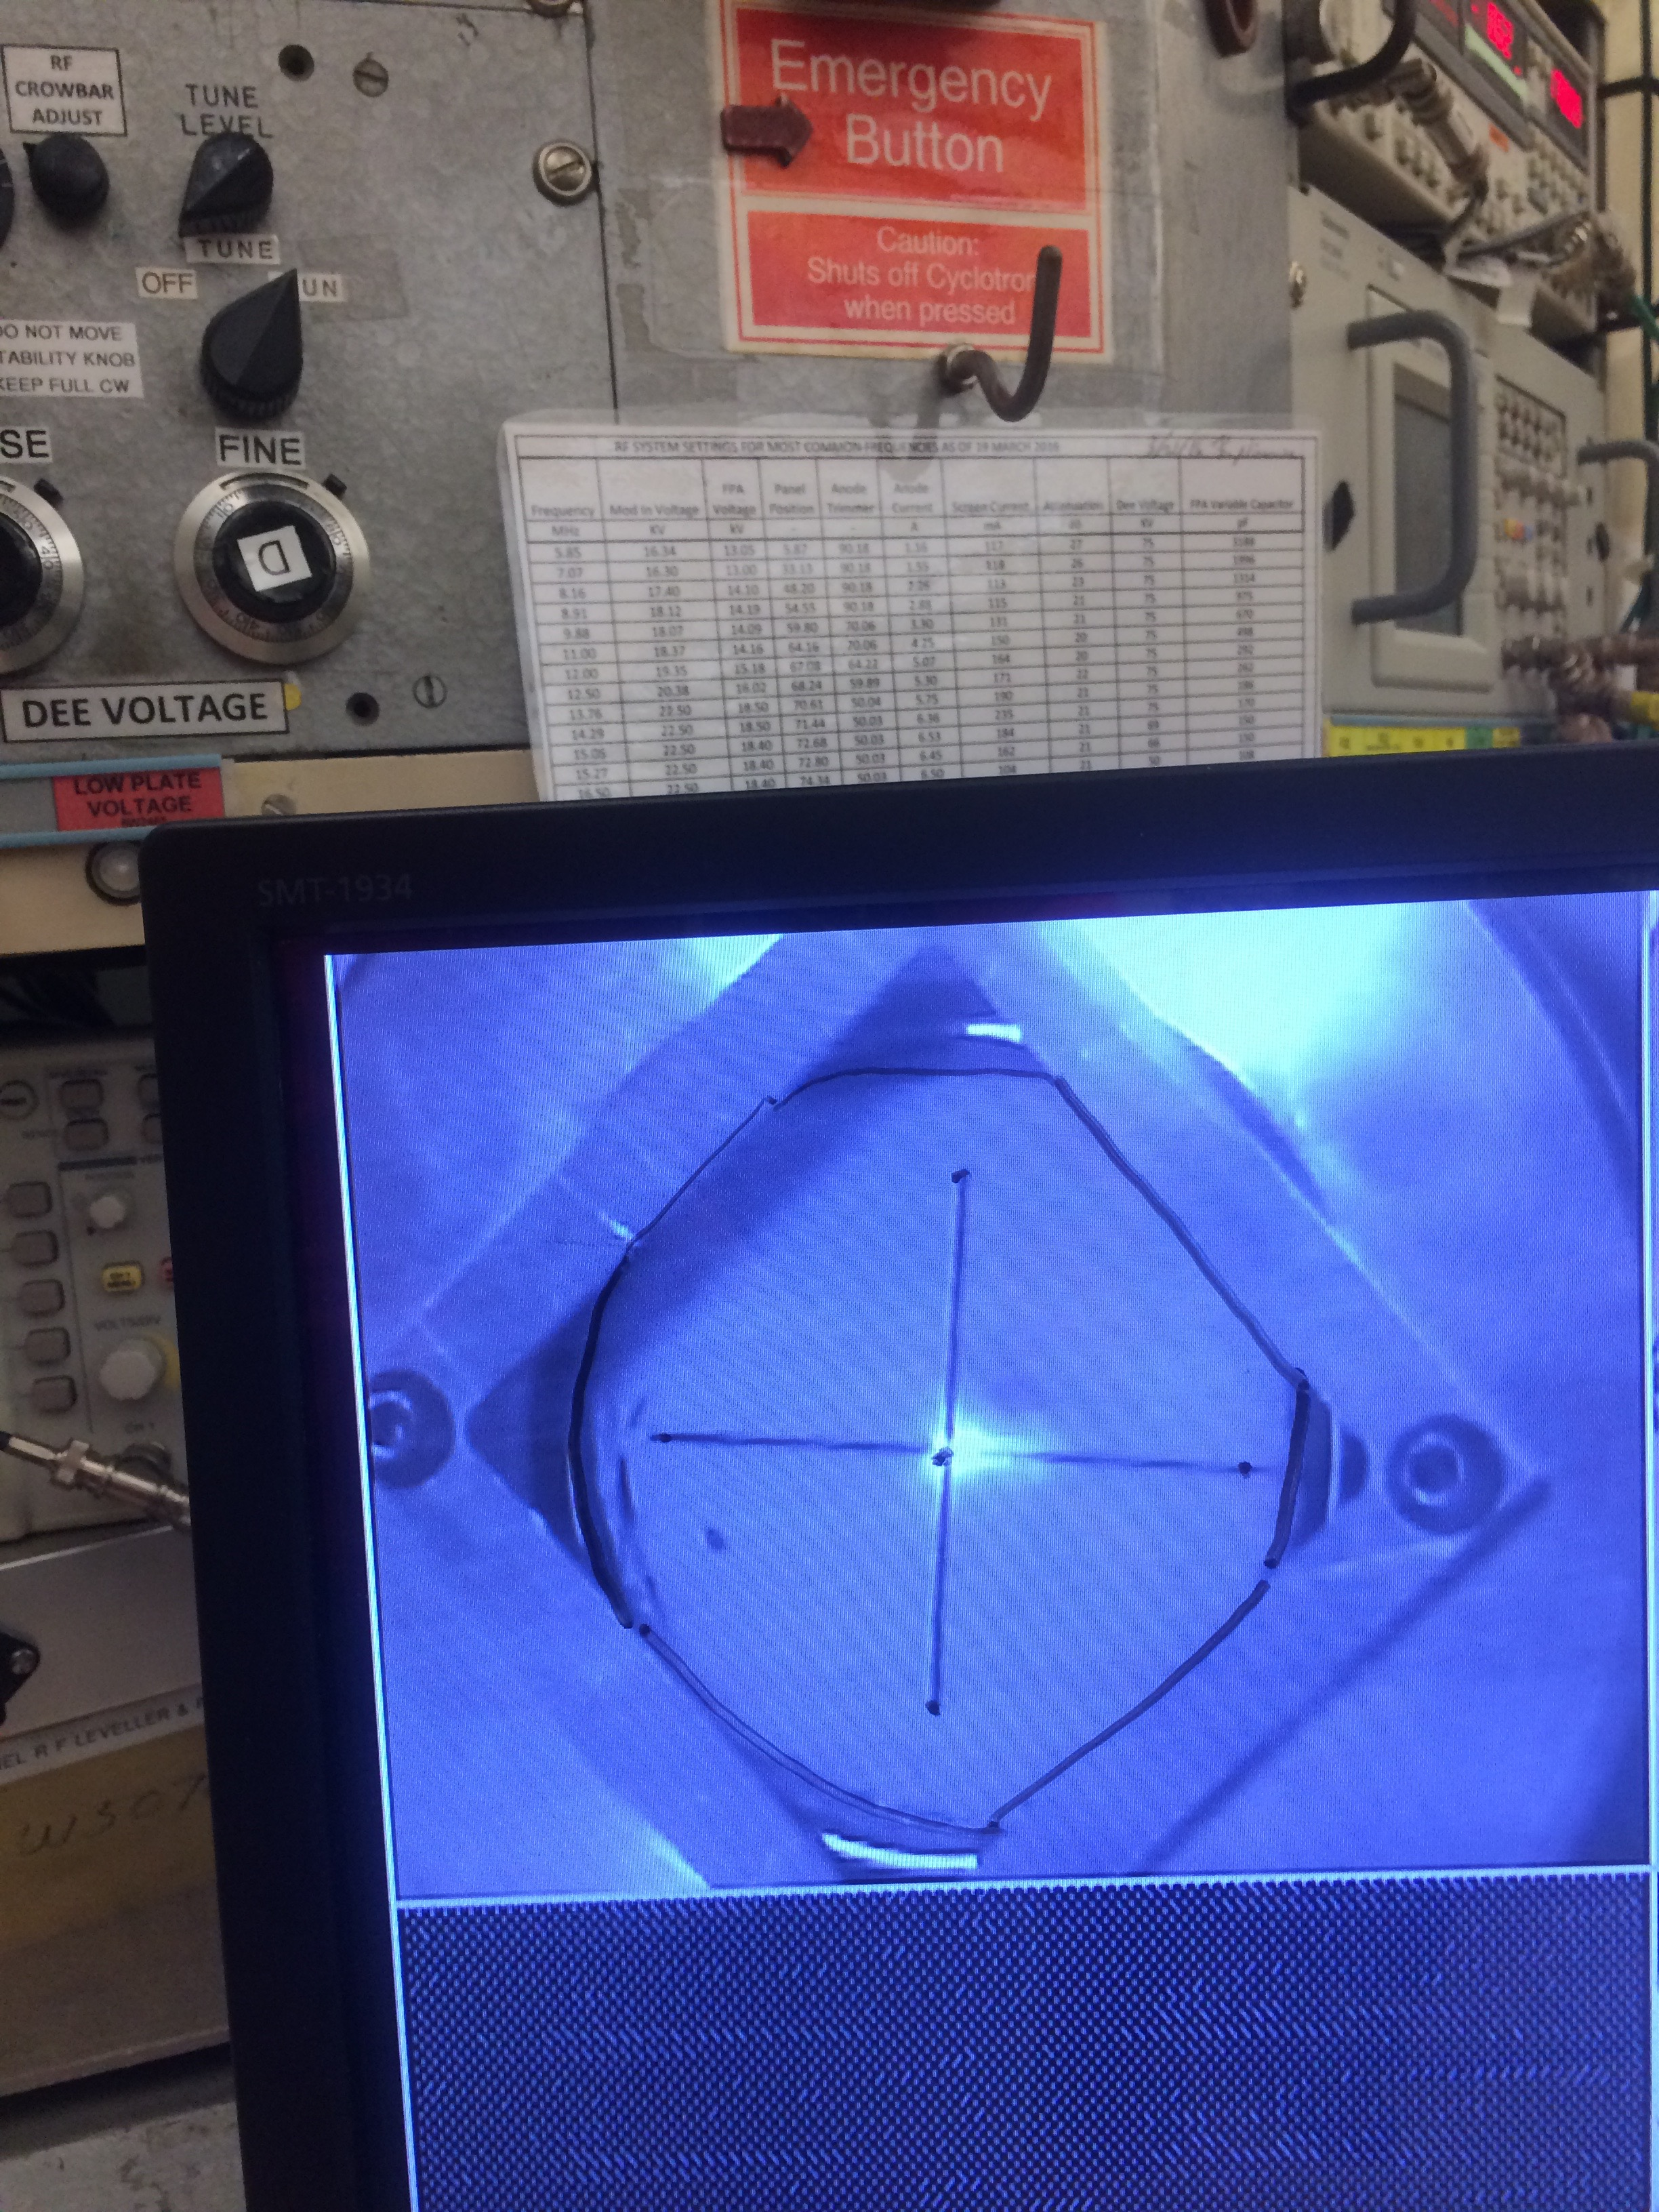
\includegraphics[width=0.75\columnwidth]{./figures/IMG_0337.jpg}
 % IMG_8840.JPG: 4032x3024 pixel, 72dpi, 142.24x106.68 cm, bb=0 0 4032 3024
 \caption{View of the remote feed of the phosphor target during beam optics tuning. The low-current proton beam used for tuning is visible as the bright glow around the reference crosshairs.}
 \label{fig:fe_preexp_beam_spot}
\end{figure}



\begin{figure}
 \centering
%                                l   b      r    top
%  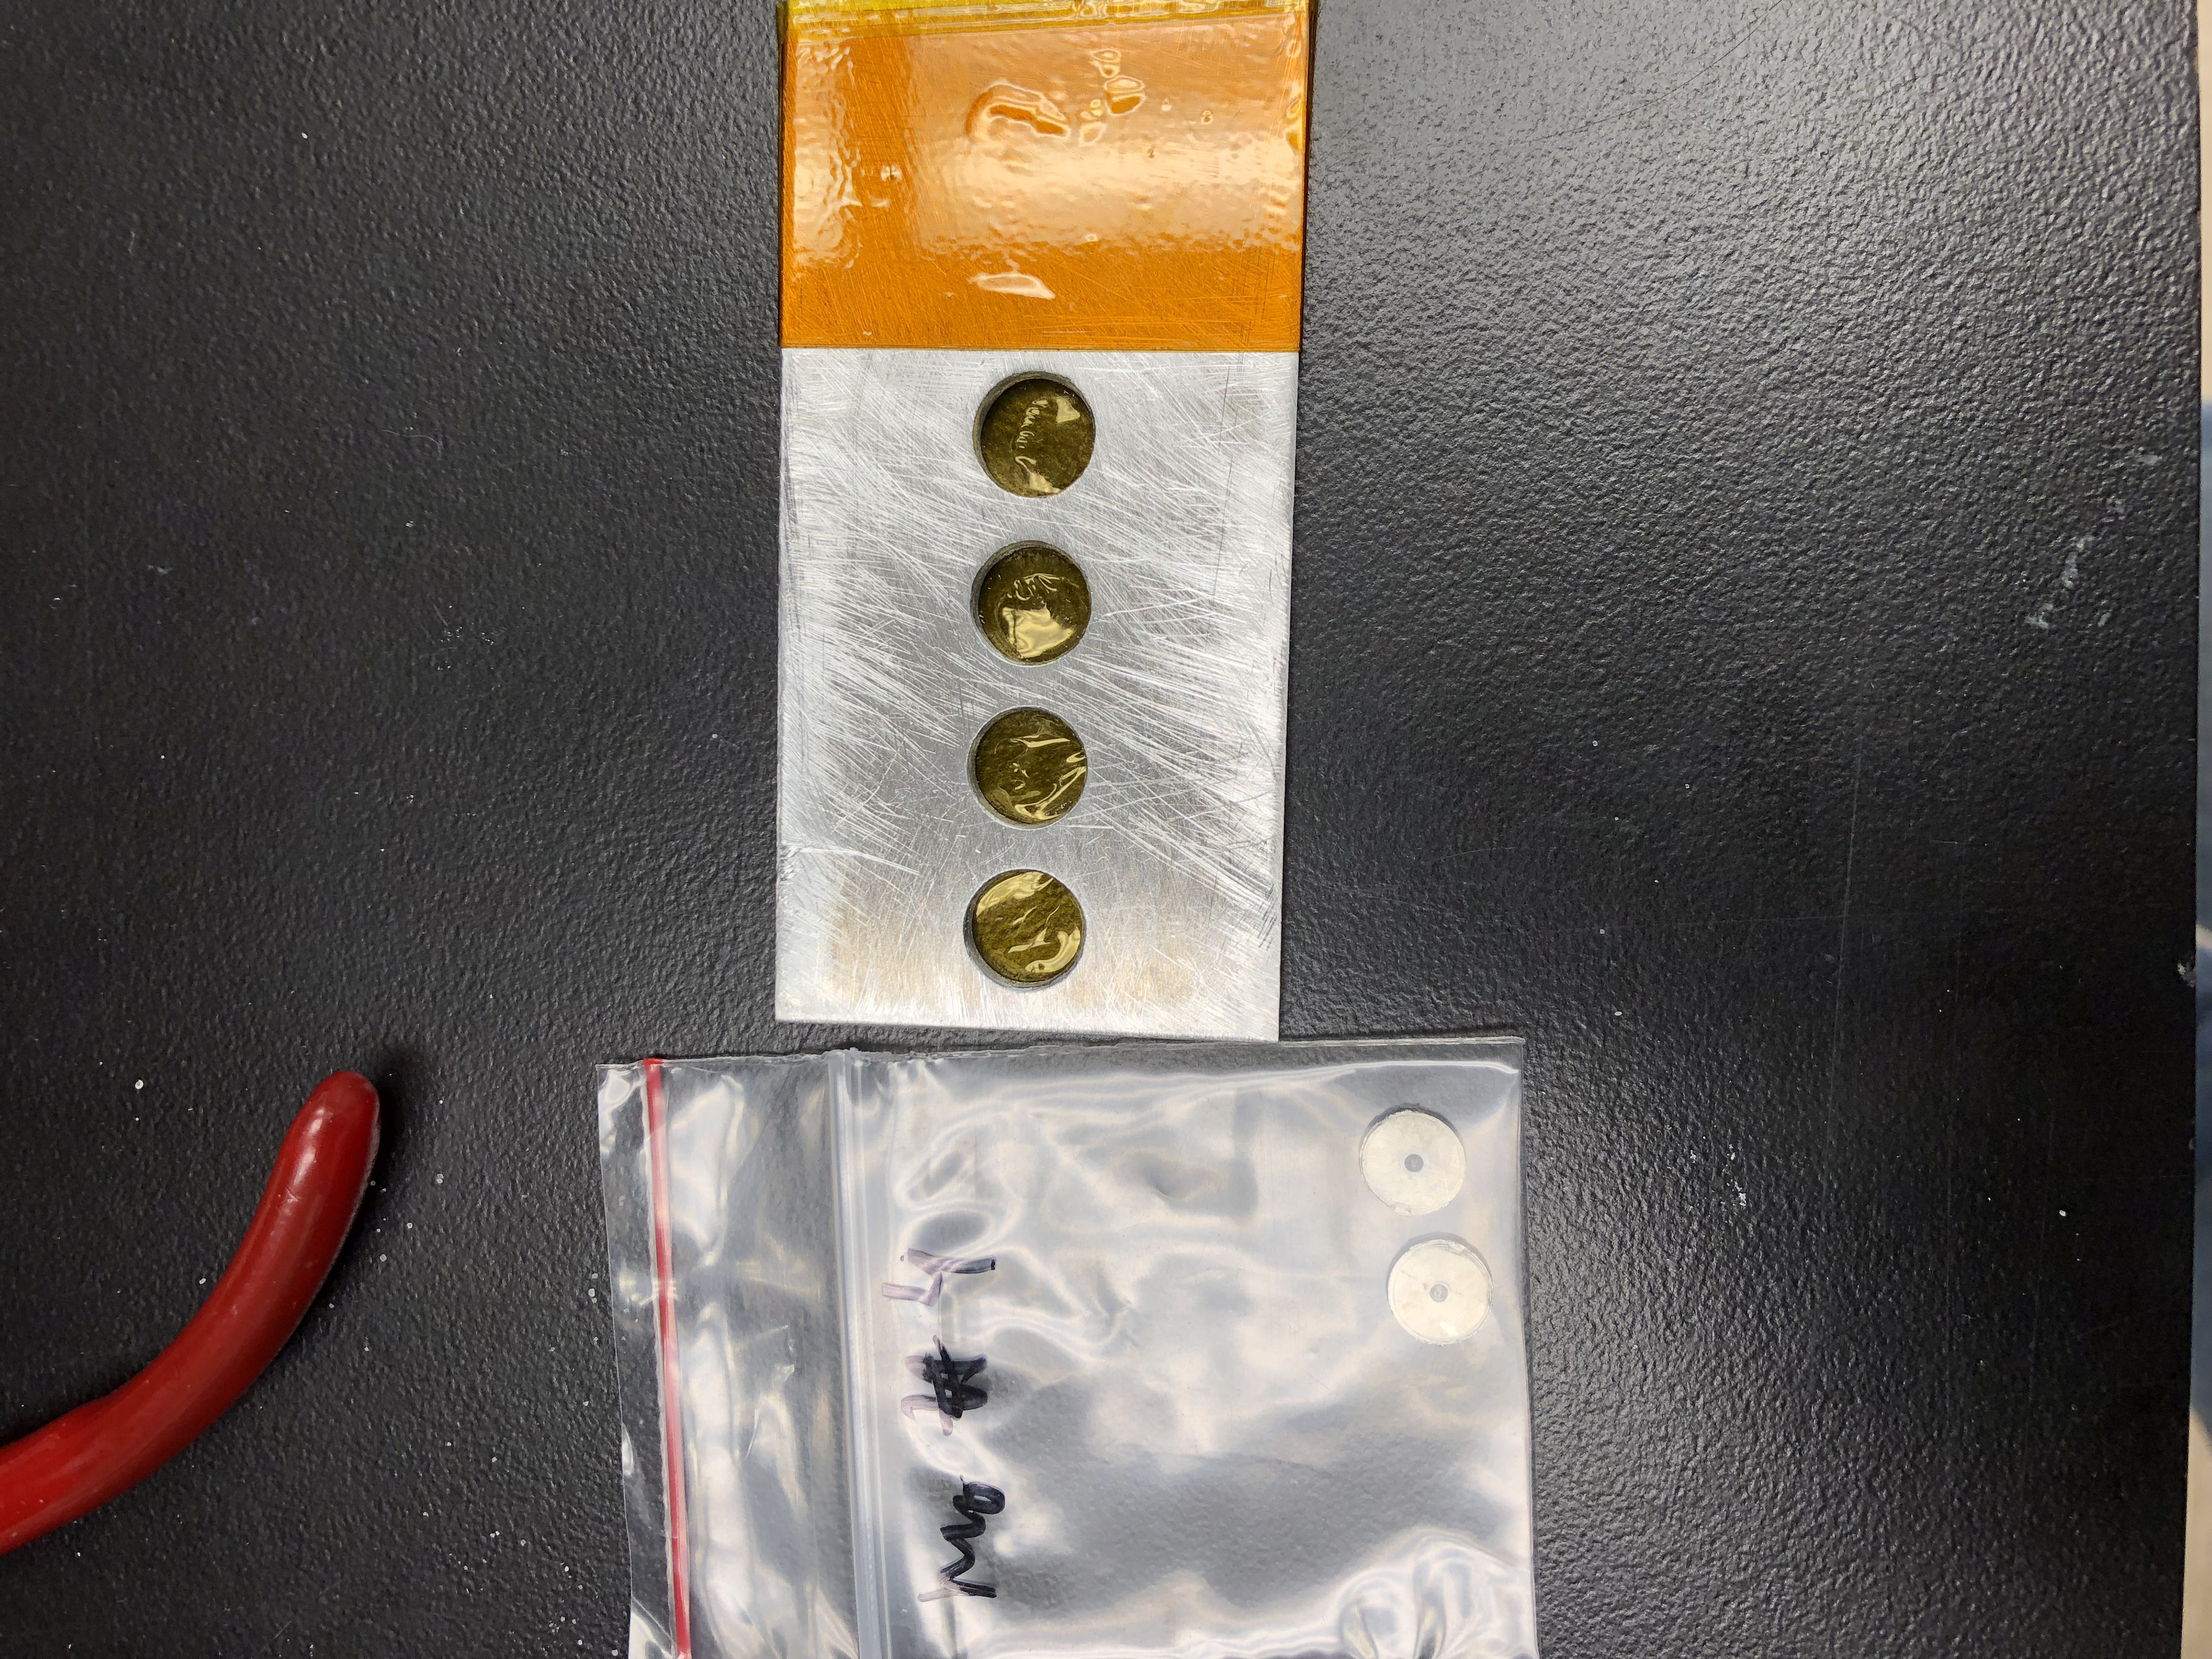
\includegraphics[clip=true,trim=5pt 1000pt 10pt 900pt,width=0.75\columnwidth,angle=90]{./figures/IMG_8840.JPG}
%  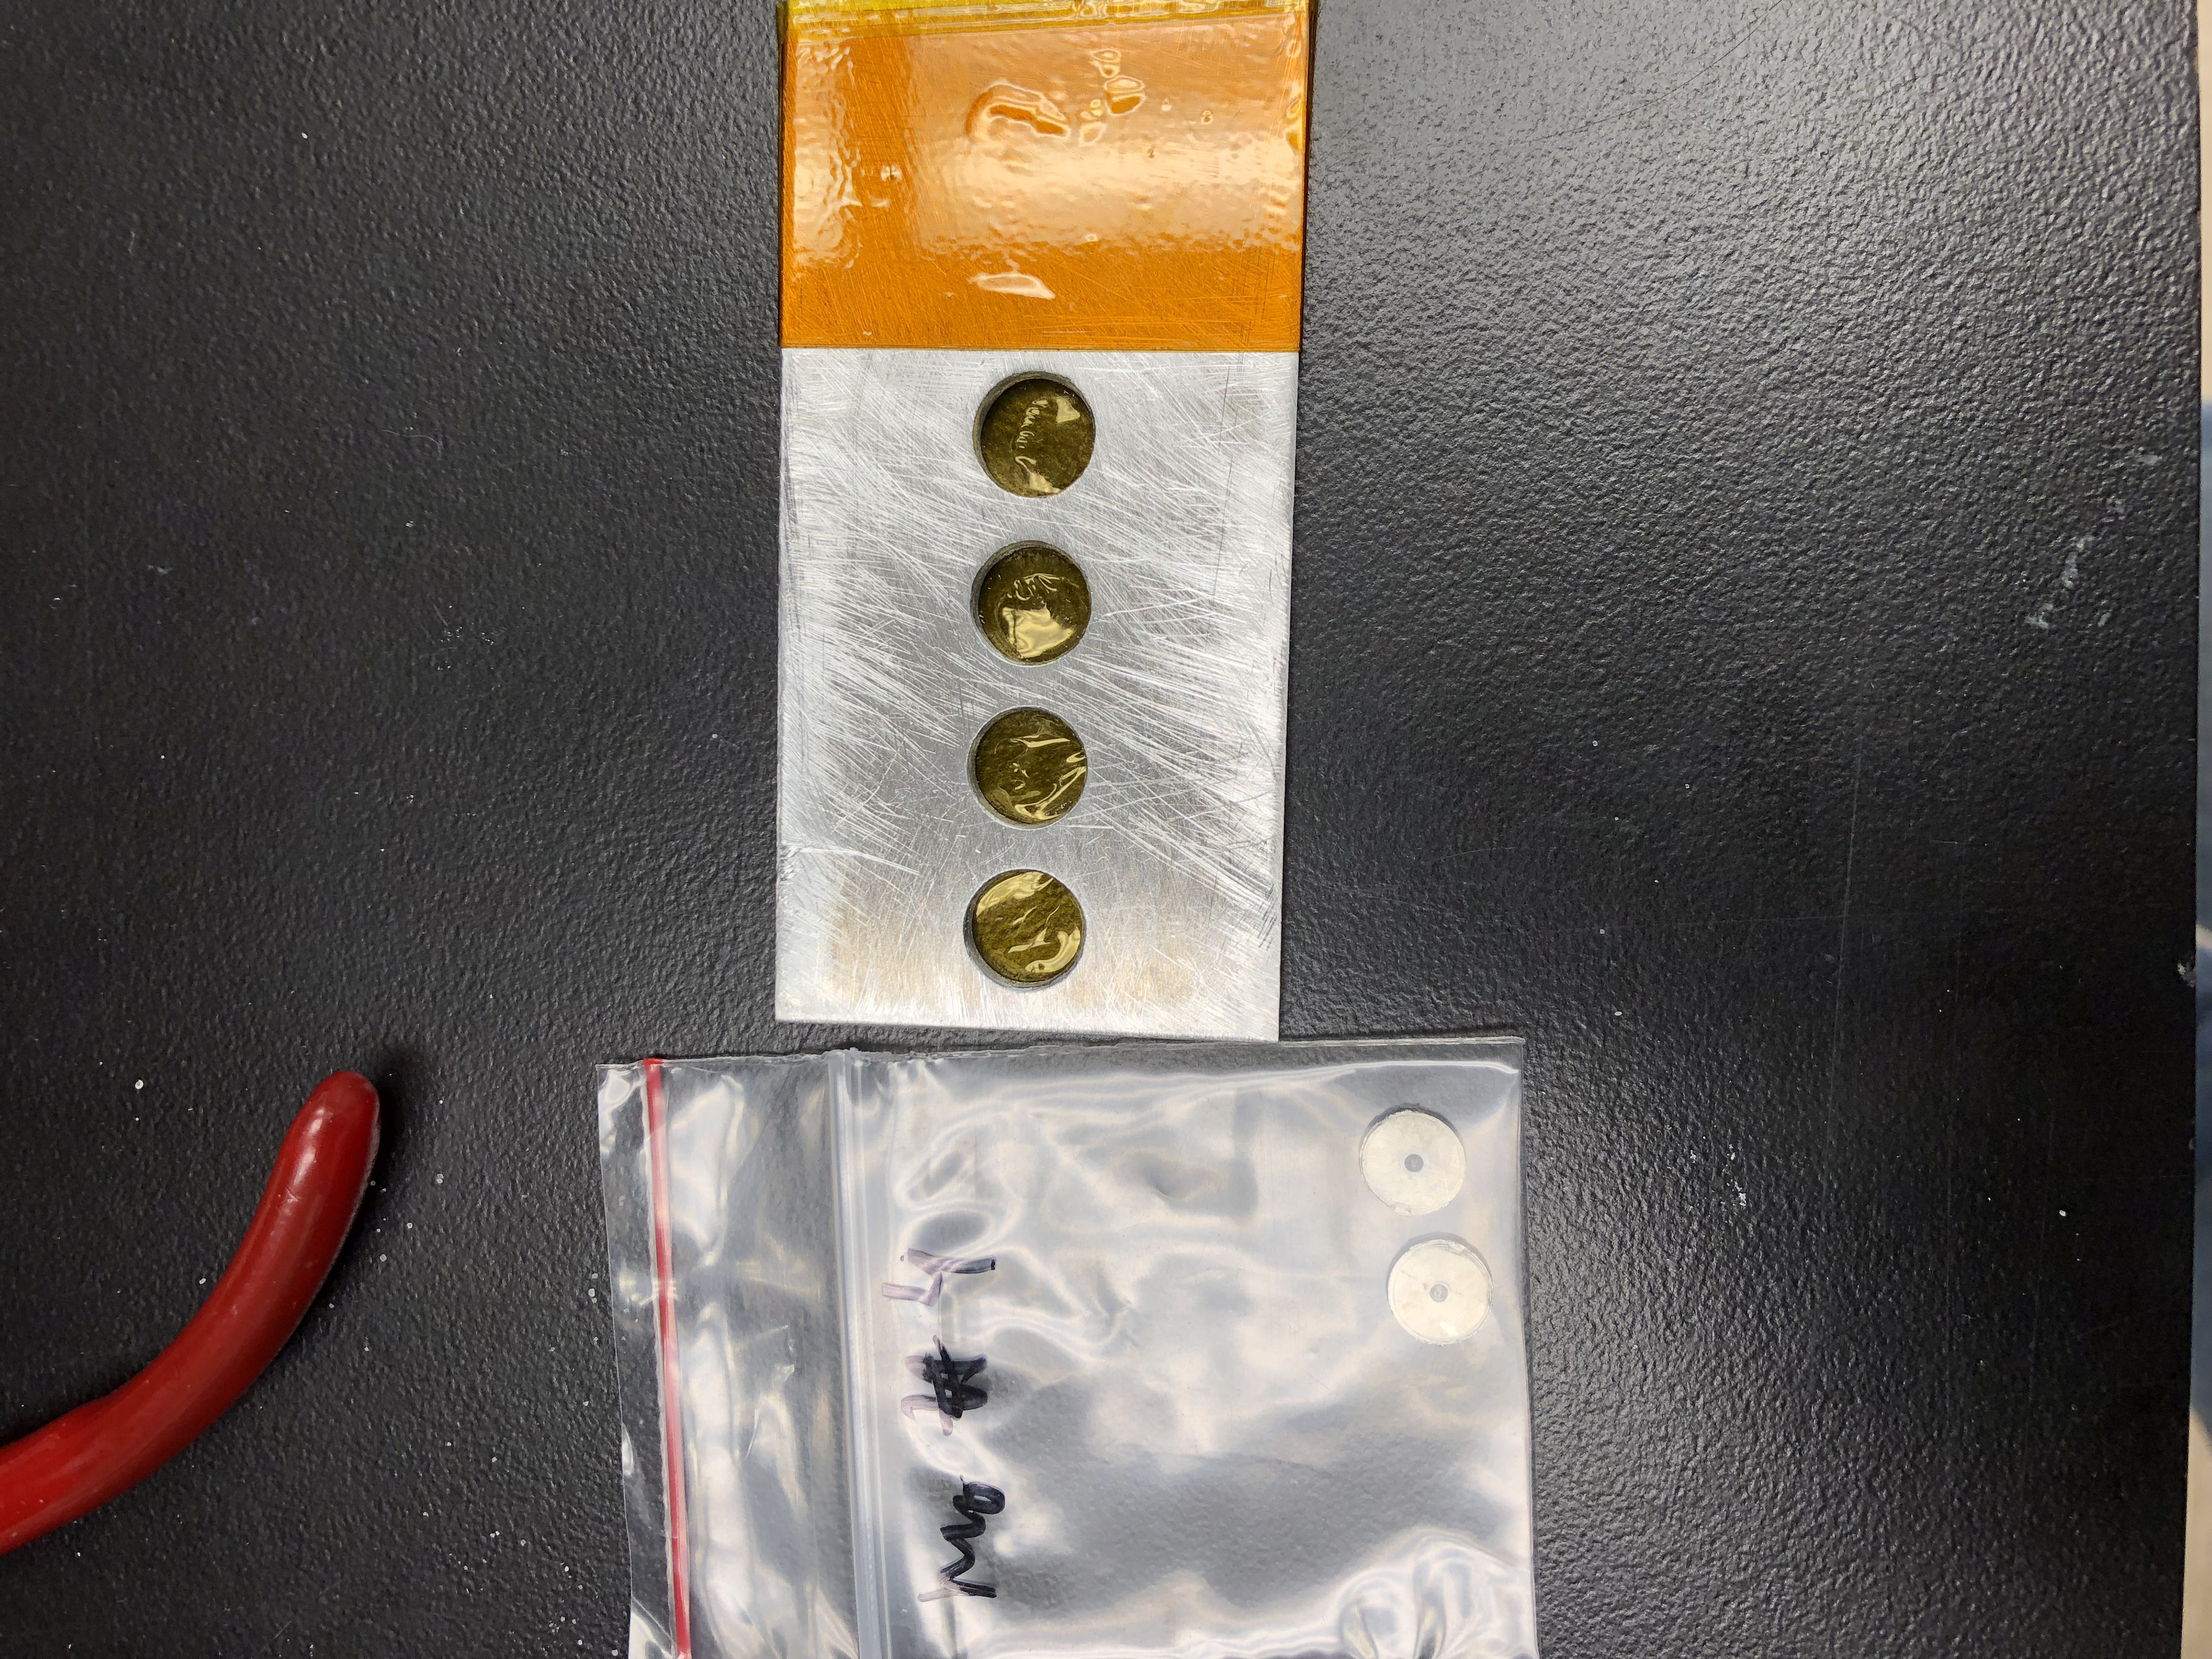
\includegraphics[width=0.75\columnwidth,angle=270]{./figures/IMG_8840.JPG}
 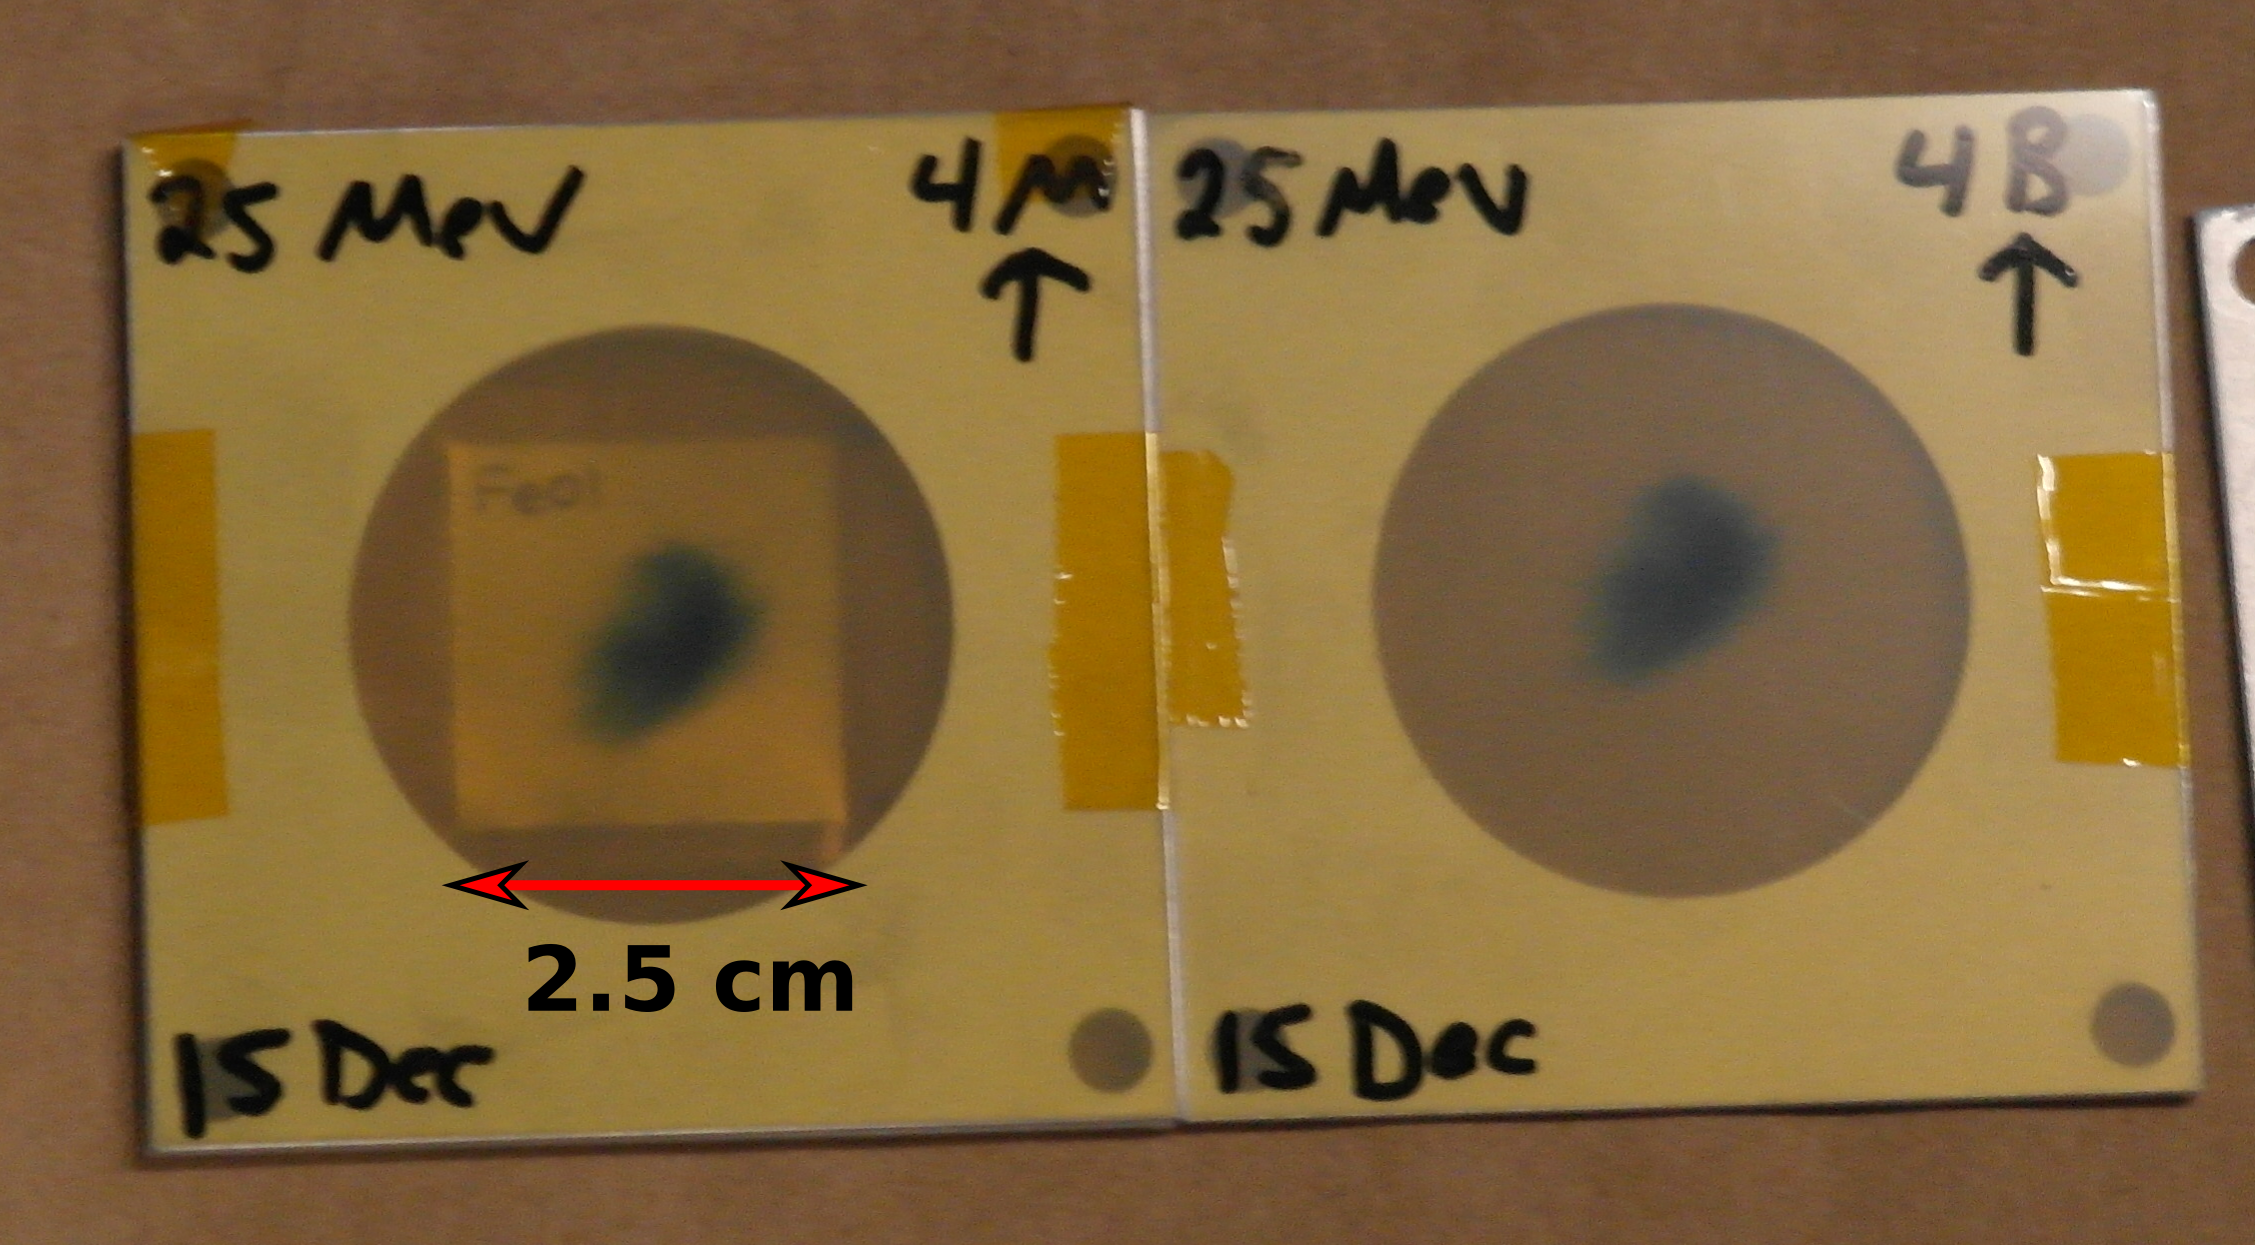
\includegraphics[width=0.75\columnwidth]{./figures/25MeV_optics_films.png}
 % IMG_8840.JPG: 4032x3024 pixel, 72dpi, 142.24x106.68 cm, bb=0 0 4032 3024
 \caption{Final beam spot profile for the 25\,MeV LBNL Fe(p.x) measurement. The  proton beam is confirmed to be centered on the target position, and is focused to underfill the 25$\times$25\,mm target foils.}
 \label{fig:fe25_preexp_beam_spot}
\end{figure}

\begin{figure}
 \centering
%                                l   b      r    top
%  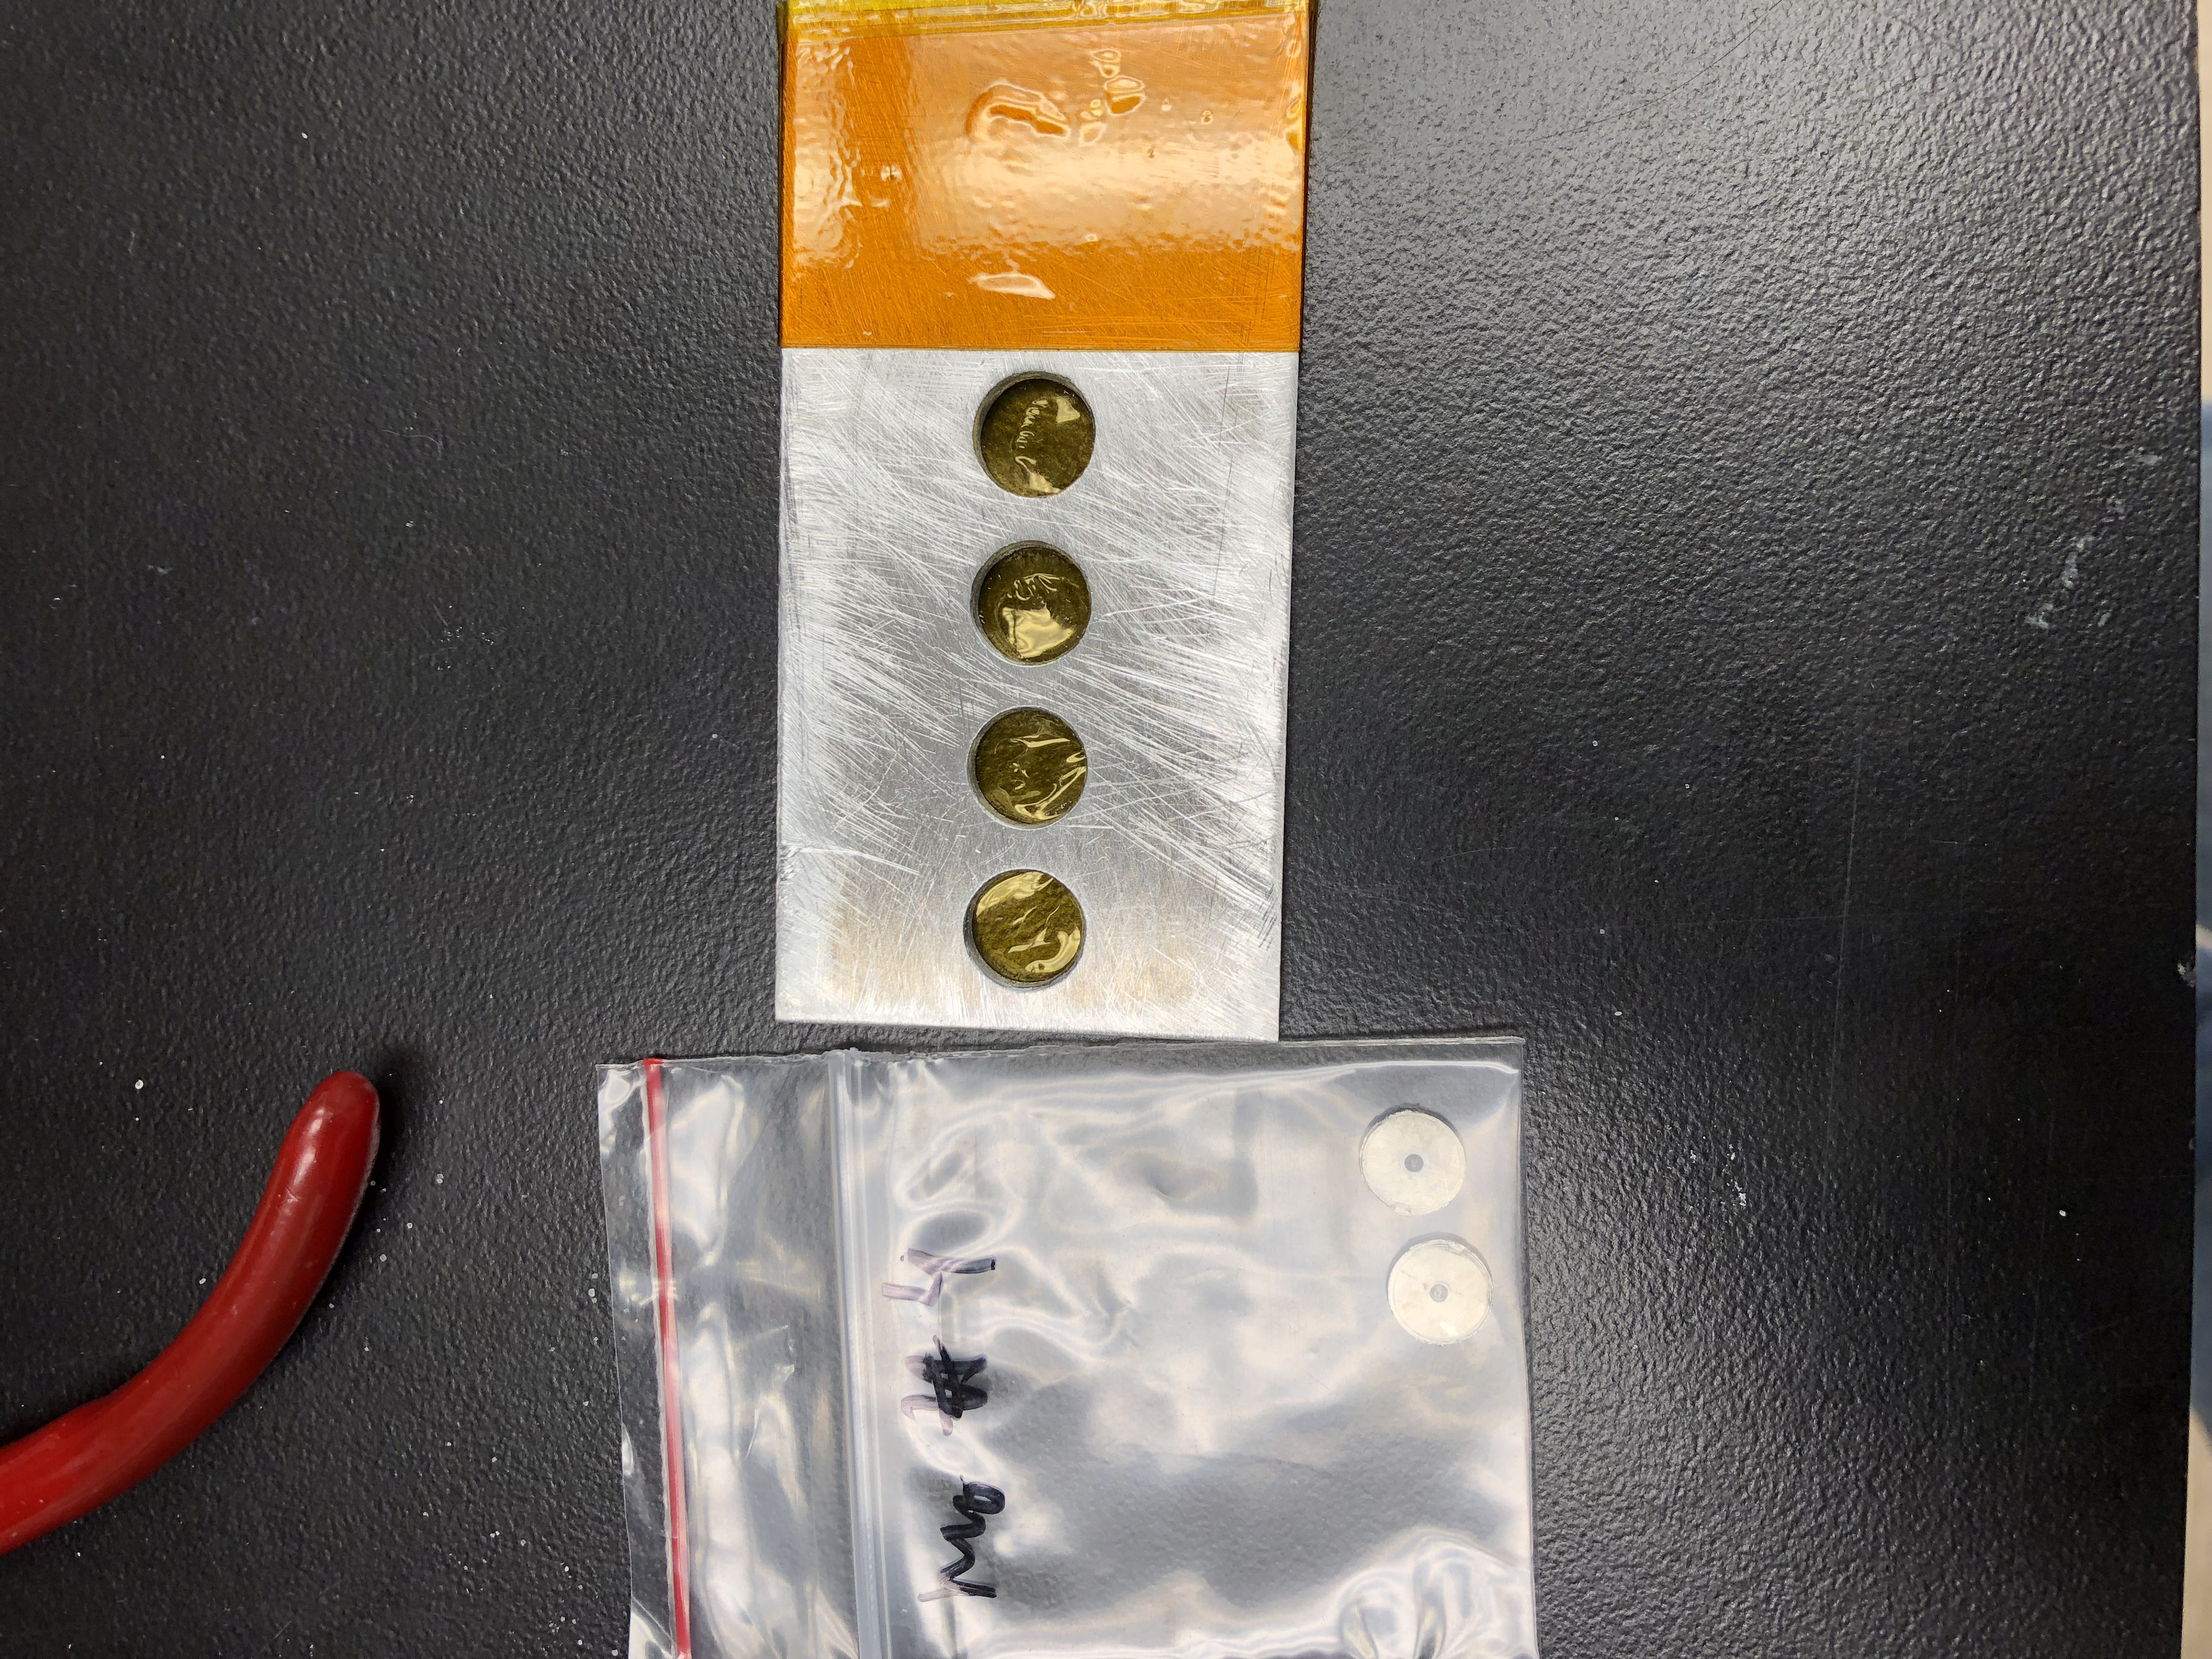
\includegraphics[clip=true,trim=5pt 1000pt 10pt 900pt,width=0.75\columnwidth,angle=90]{./figures/IMG_8840.JPG}
%  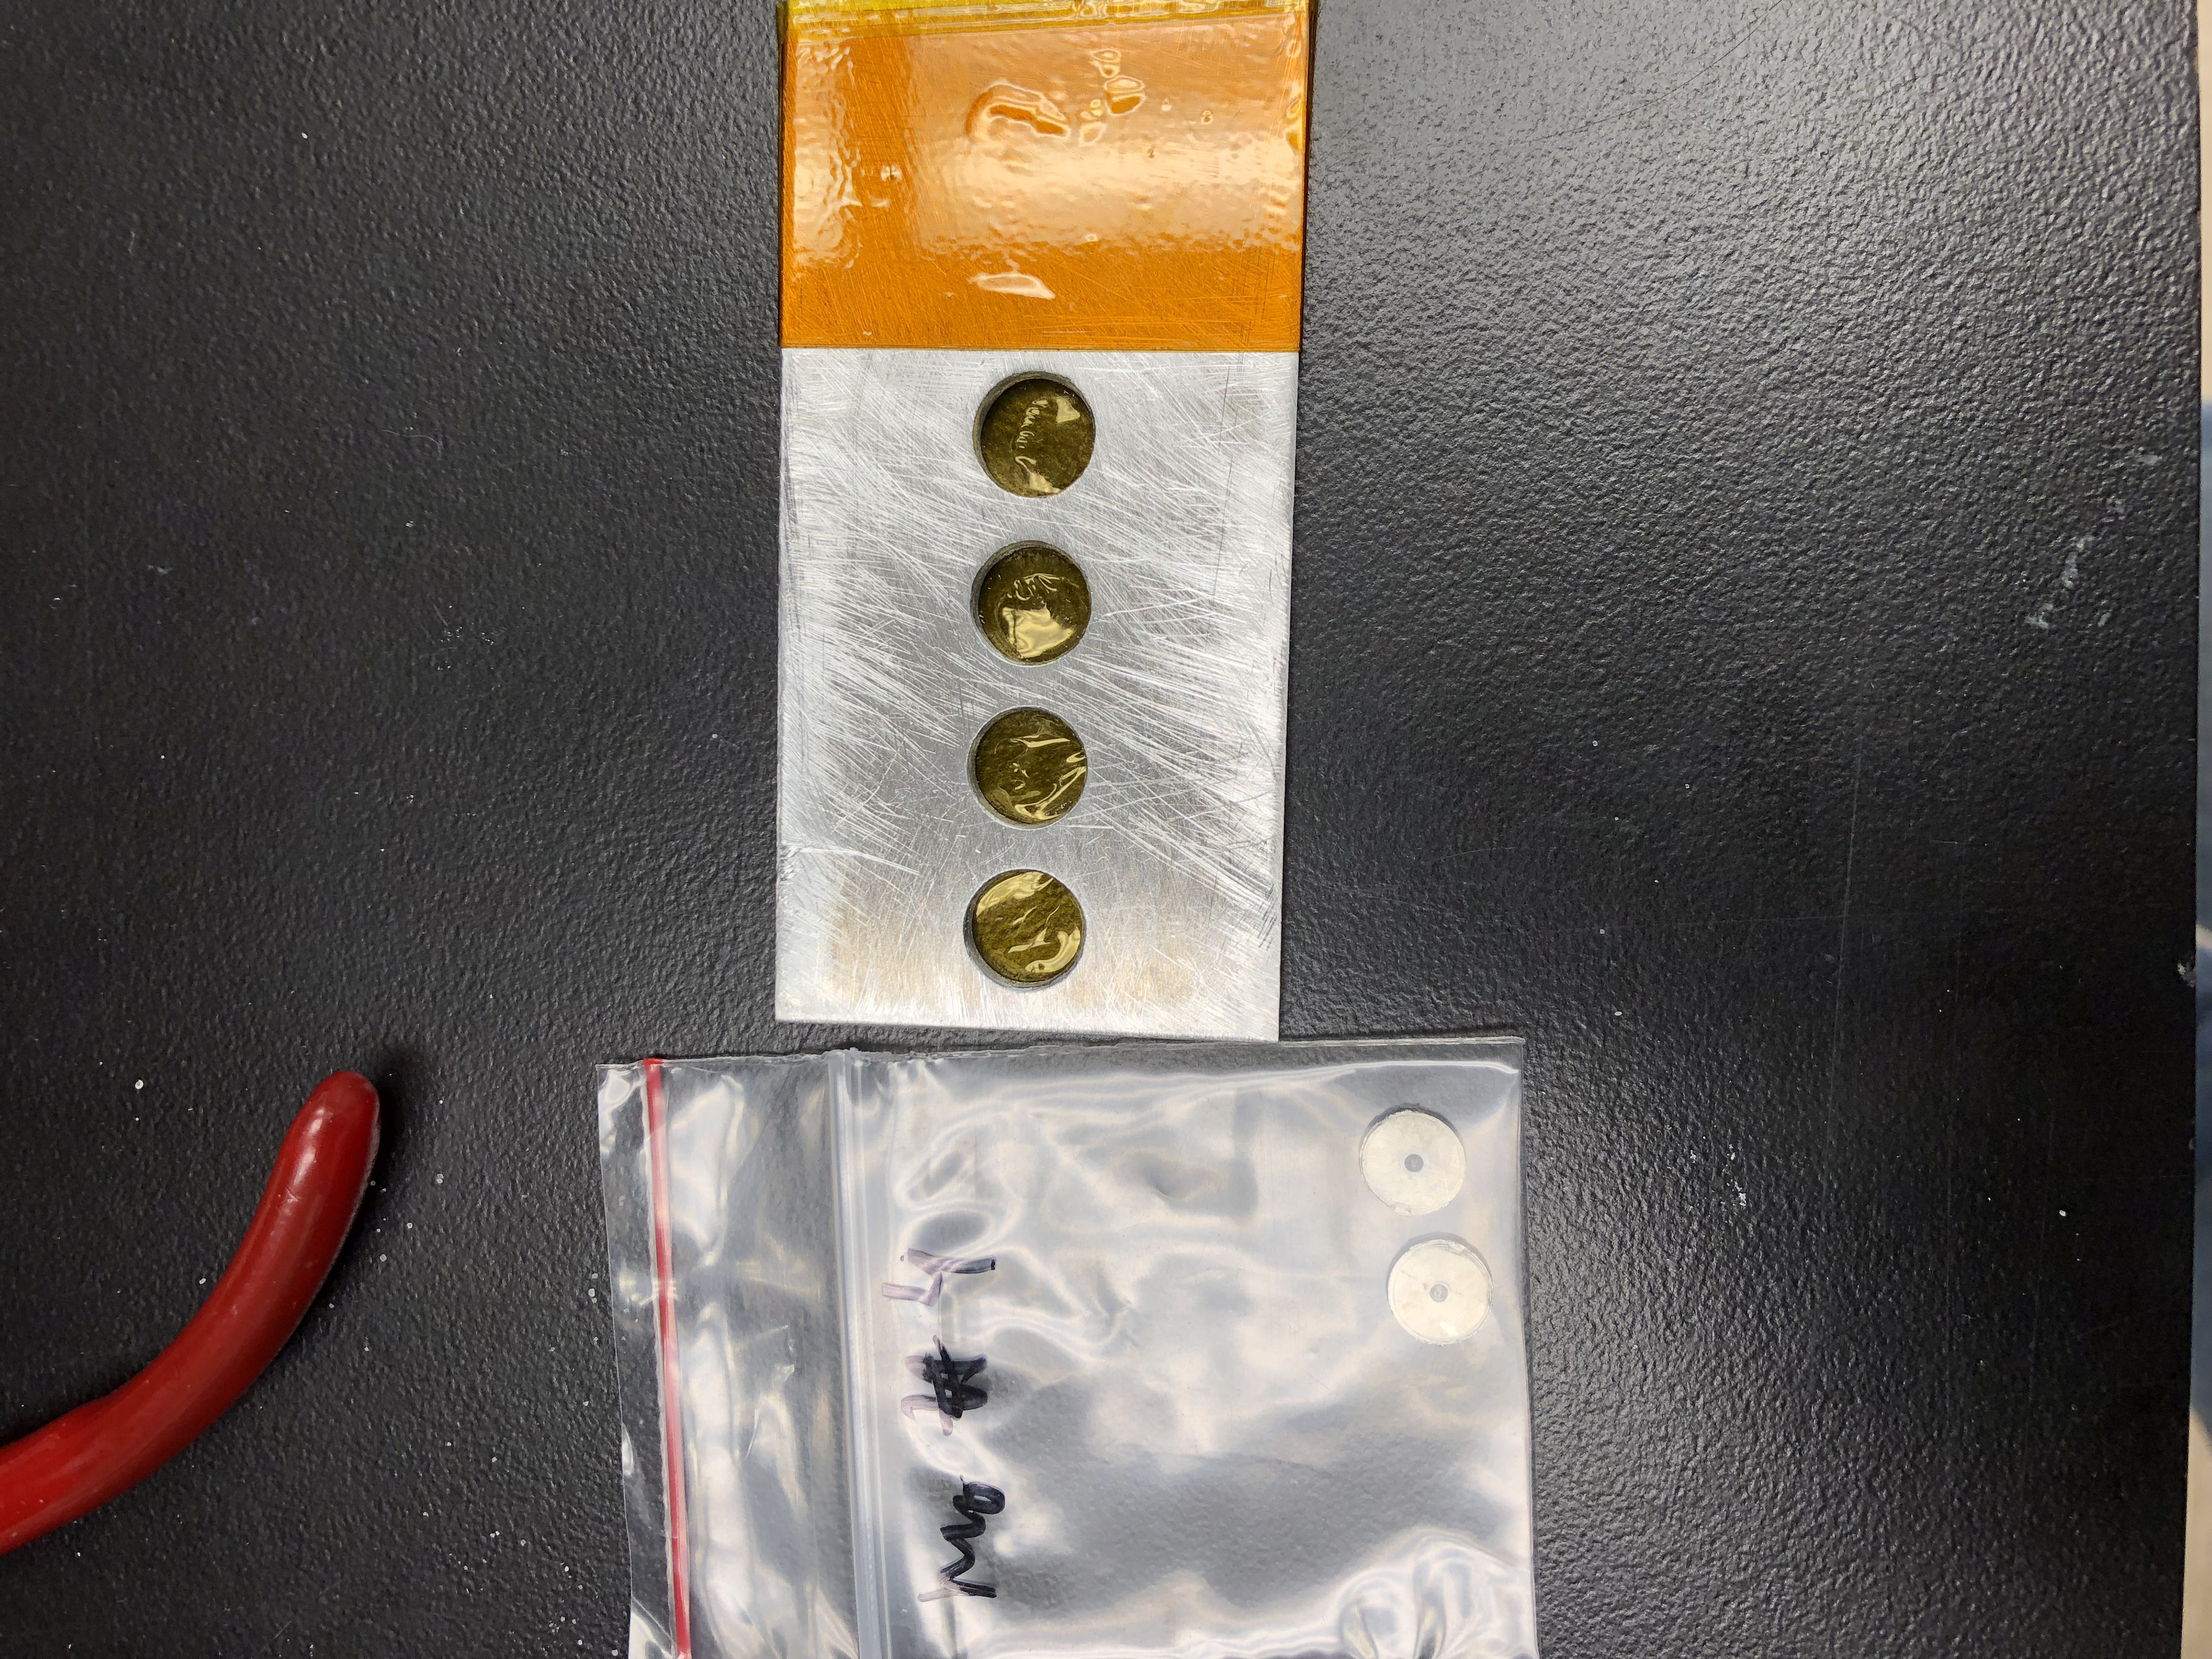
\includegraphics[width=0.75\columnwidth,angle=270]{./figures/IMG_8840.JPG}
 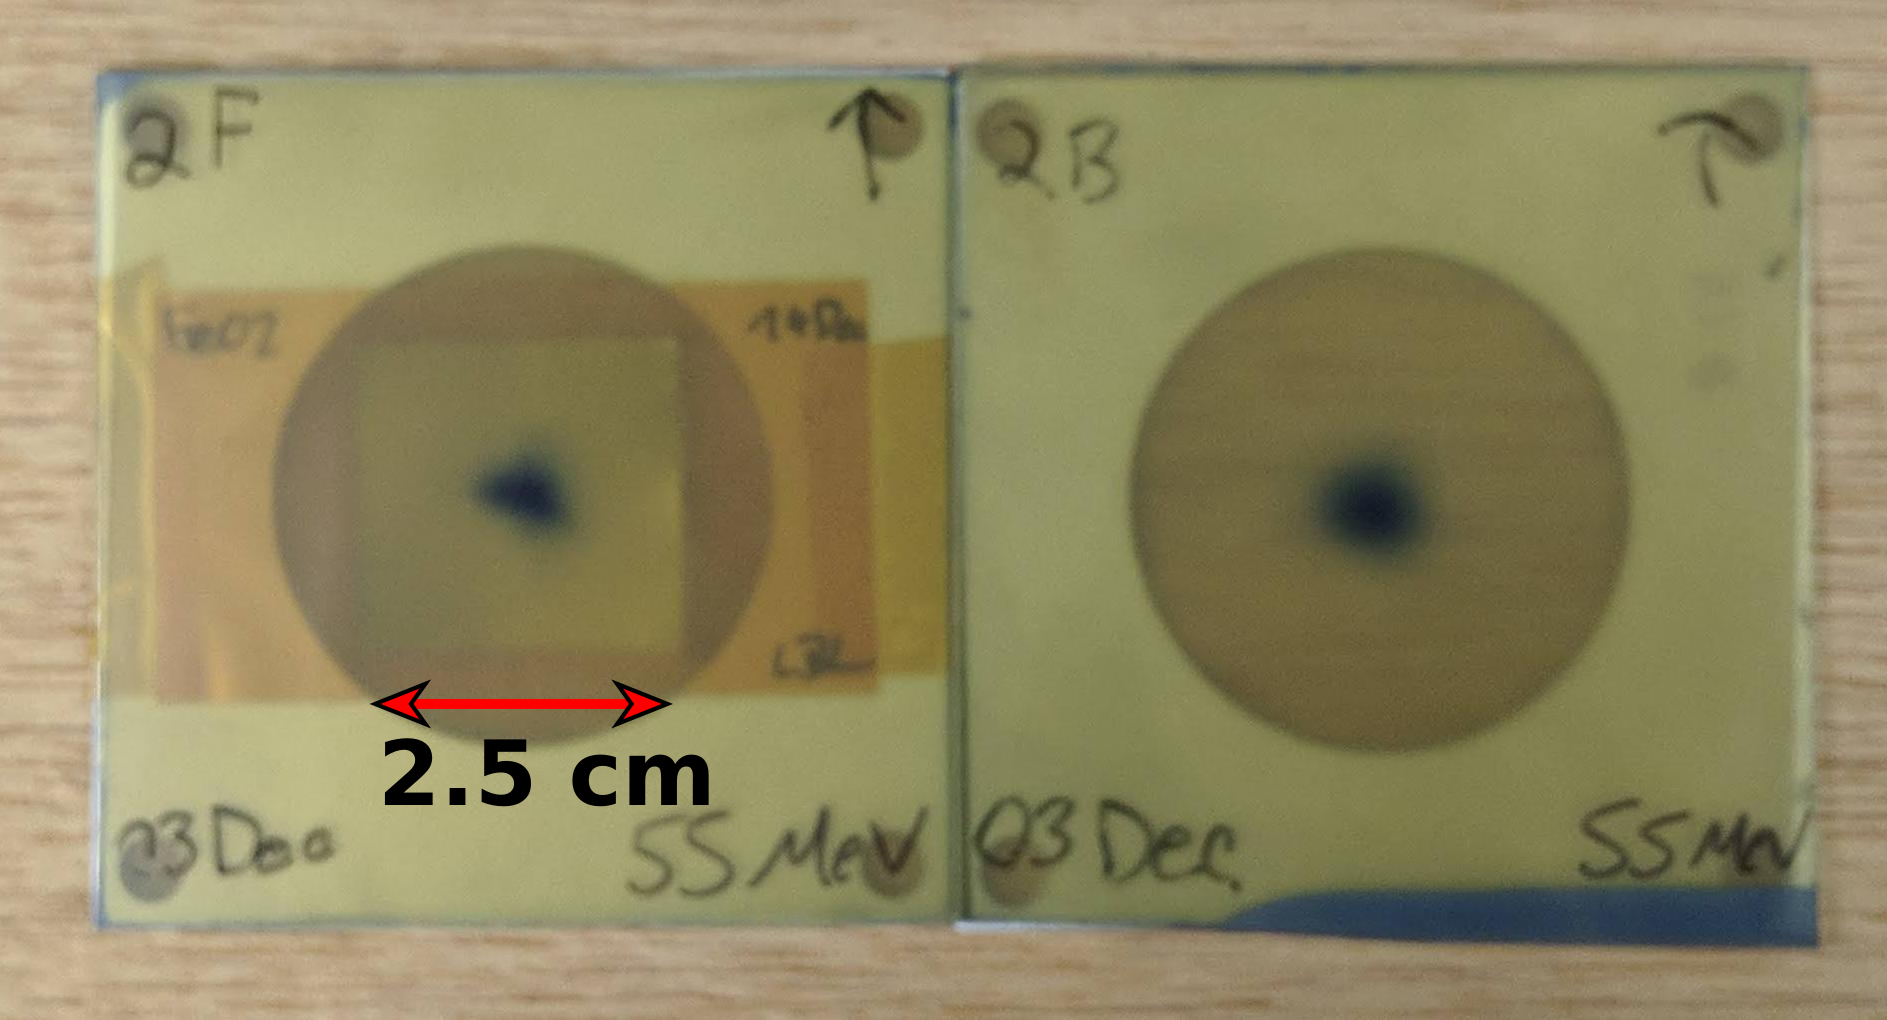
\includegraphics[width=0.75\columnwidth]{./figures/55MeV_optics_films.png}
 % IMG_8840.JPG: 4032x3024 pixel, 72dpi, 142.24x106.68 cm, bb=0 0 4032 3024
 \caption{Final beam spot profile for the 55\,MeV LBNL Fe(p.x) measurement. The  proton beam is confirmed to be centered on the target position, and is focused to underfill the 25$\times$25\,mm target foils.}
 \label{fig:fe55_preexp_beam_spot}
\end{figure}





These films are useful for determining the beam profile incident upon the front of each stack.
However, the beam broadens as it traverses the target stack, with large-angle deflections (primarily in the aluminum degraders) from scattering of the beam.
To image the actual beam profile incident upon the first foil in the stack (Fe-01 and Fe-08), a 316 stainless steel foil (SS-3 and SS-5) is inserted upstream of Fe-01 and Fe-08, for the 55 and 25\,MeV stacks, respectively, to serve as a beam profile monitor for the activation foils.
Likewise, another stainless steel profile monitor (SS-4 and SS-6) is inserted downstream of the last foil in the stack (H-02 and Cu-20).
These stainless steel monitors are cut to the same length and width as the aluminum frames used for mounting foils, and are characterized in \autoref{tab:fe_stack_table}.





As described in \autoref{sec:target_design_fe}, decay radiation emitted from the activated stainless steel foils were used to develop radiochromic film (Gafchromic EBT3), revealing the spatial profile of the beam entering and exiting the stack.
% Radiochromic films, such as Gafchromic EBT, come in multiple varieties, depending on the   dose range and the type of ionizing radiation desired to provide sensitivity to. 
% In general, such films are commonly self-developing, containing a radiation-sensitive organic polymer dye as the active layer.
% This dye, much like the polyethylene beam profile monitors, is damaged by ionizing radiation, with multiple free radicals initiated in the process.
% These free radicals result in cross-linking, breaking of double bonds, and fragmentation of the dye polymer, which causes the damaged dye to undergo a large visible change in  color.
% The intensity of this color change is often proportional to the dose received by the film, and is preferred to be energy-independent \cite{Azam1998}.
% Many such films are sensitive to prolonged UV exposure, and will slowly develop if not kept in a  cool, dark environment, leading to systematic errors in observed dose.
% The thin dye layer in most films is extremely sensitive, so care must be taken to avoid bending or deforming, which can make them insensitive to development when irradiated.
% % Following exposure, the film may be scanned 
% For reference, the Gafchromic EBT film used in this work is comprised of a pair of 25\,\mmicro m active layers containing the radiation-sensitive EBT emulsion dye, separated by a 3\,\mmicro m surface layer and sandwiched in between a pair of 97\,\mmicro m layers of clear polyester, acting as a supportive and protective backing. 
% 
% 
% 
% 
% 
% 
% %  Move these first two commented sentences into PhD thesis.
% % 
% % % % 
% % An accurate integrated proton current is one of the most important factors in performing high-fidelity cross section measurements.
% % At the time of this work, the nondestructive beam current monitors in the LANSCE-IPF beamline had a  resolution of 100 nAh.
% % For a low-current irradiation such as this work, where a nominal fluence of 200 nAh is desired, additional fluence sensitivity is thus needed to accurately normalize quantified EoB activities into cross sections.
% 
The radiochromic films developed by the 55\,MeV stack's SS-3 and SS-4 stainless steel beam profile monitors are seen in \autoref{fig:gafchromic_fe}.
In addition, extra iron target foils mounted on  aluminum frames are superimposed behind each film, to guide the eye.
It is clear from the upstream (SS-3) film that the proton beam profile was consistent with that seen in the final pre-irradiation beam spot check of  \autoref{fig:fe55_preexp_beam_spot}.
The downstream (SS-4) film  reveals that the beam was not completely attenuated,  
% in the target stack
and clearly displays the  broadening expected due to scattering in the target stack. 
More importantly, the beam profiles in both films appear to be completely contained within the 25$\times$25\,mm activation foils, including the beam envelope.
As discussed previously in \autoref{sec:nb_profile_measurements}, this confirms that the activation foils were exposed to  the total beam current.


% If the beam were to be misaligned on the foils, or were to have sufficiently broadened such that it greatly overfilled the foils, the activation foils would be exposed to only a fraction of the total beam current.
% If  fluence measurements are purely taken from an external  current monitor (such as an inductive pickup upstream of a target, or an electrically-isolated target in a Faraday cup), the  fraction of current which misses the foils will not be detected.
% This leads to reporting a false, larger  fluence, which will cause all cross sections to be erroneously reported with a reduced magnitude.
% Thus, it is for this  reason that having monitor foils at each energy position builds confidence in reported cross sections, as they serve to screen for systematic errors such as this.
% However, profile monitors play a vital role in the detection of lost beam fluence when monitor foils are unavailable. 
% Additionally, 







% Since the color change developed by irradiation is proportional to the dose deposited in the film, the optical density of the film may be used to measure dose.
% In clinical external-beam radiation therapy, these films are commonly used in quality assurance  to map and verify  the dose contours for therapeutic gamma-ray fields.
% However, the dose sensitivity of these films is often greater than the ability to be visually distinguished beyond simple qualitative inspection.
% As a result, following exposure, the film may be digitized using any flatbed scanner.
% Image analysis may be thus used to measure the optical density profile as a surrogate for dose or beam intensity profiles.
% The optical density is often fit to a curve of the form
% \begin{equation}
% d_x\pp{D} = a + \dfrac{b}{D-c}
% \end{equation}
% where $d_x\pp{D}$ is the optical density of exposed radiochromic film in scanner color channel $x$ at dose $D$, and $a$, $b$, and $c$ are calibration parameters.
% Using a standard irradiation source (commonly a collimated \ce{^{60}Co} source), a calibration curve can thus be measured to convert optical density into an absolute dose.
% This is most common in clinical and quality assurance applications.
% In addition, modern radiochromic films are often designed such that the characteristic exposure curve for the active layer dye differs between the red, green, and blue color channels, offering even further enhanced sensitivity to dose \cite{bushberg2011essential,Andre2011,David2012}.




% However, for cases where an absolute dose is not necessary, the optical density can still be used for a qualitative measure of relative beam intensity, or relative dose.
Using the image analysis code  ImageJ-2.0.0,  profiles of the total optical density were extracted for both the SS-3 and SS-4 radiochromic films \cite{Rueden2017}.
These are seen in \autoref{fig:gafchromic_fe_profiles}, as relative beam intensity profiles along the major and minor axis of each film.
As seen visually, for both axes, the peak beam intensity drops from SS-3 to SS-4, as the proton fluence is clearly broadened by scattering reactions in the target stack.
% As seen visually, there is a clear broadening of the beam spot in the rear of the target stack.
Along the major (\enquote{horizontal}) axis, the FWHM of the beam profile slightly broadens from 0.431\,cm to 0.516\,cm, and along the minor (\enquote{vertical}) axis, the FWHM of the beam profile broadens from 0.396\,cm to 0.473\,cm.
In addition, the centroid position of the minor axis clearly appears to  shift by approximately 0.46\,cm between the front and rear of the stack. 
The measured beam profiles were fit using a Gaussian model with linear background, to aid in comparing the widths of each profile.
The Gaussian model does well to fit the beam profiles overall, though it overestimates the peak height for a given Gaussian width.
This is likely due to the fact that the beam itself has an intrinsic spatial width before any interactions with the target stack; this leads to more broadening of the beam envelope than of its core.

    

% 55\, MeV
% 
\begin{figure}
    \centering
    \subfloat{
        \centering
%         \includegraphics[width=\columnwidth]{./figures/Capture.PNG}
        \hspace{-5pt}\subfigimg[width=0.5\textwidth]{a)}{./figures/DOC073018_SS3-cropped.pdf}{80}
%         \caption{ Decay curve for the isomeric transition of \ce{^{115m}In}.}
         %         \refstepcounter{subfigure}
         \label{fig:gafchromic_fe_upstream}
   \hspace{-5pt}}%
     \subfloat{
        \centering
%         \includegraphics[width=\columnwidth]{./figures/Capture.PNG}
%         \includegraphics[scale=0.6]{./figures/391keV_curve2.png}
        \subfigimg[width=0.5\textwidth]{b)}{./figures/DOC073018_SS4-cropped.pdf}{80}
%         \caption{ Decay curve for the isomeric transition of \ce{^{113m}In}.}
         %         \refstepcounter{subfigure}
         \label{fig:gafchromic_fe_downstream}
   \hspace{-5pt}}%
    \caption{Radiochromic films for the 55\,MeV LBNL Fe(p,x) measurement, developed by the stainless steel beam profile monitors in (a) the front of the stack (SS-3) and (b) the rear of the stack (SS-4). An unused iron  foil is aligned behind each film, confirming that both the beam core and envelope underfilled the activation foils.}
     \label{fig:gafchromic_fe}
\end{figure}




\begin{figure}
    \centering
    \subfloat{
        \centering
%         \includegraphics[width=\textwidth]{./figures/target2.png}
        \subfigimg[width=0.496\textwidth]{a)}{./figures/55MeV_horz_fe_beam_profile.pdf}{50}
%         \caption{Decay curve for the $\beta^-$ decay of \ce{^{116}In}.}
        %         \refstepcounter{subfigure}
%          \label{fig:54Mn}
%
%         \includegraphics[width=\columnwidth]{./figures/Capture.PNG}
        \subfigimg[width=0.496\textwidth]{b)}{./figures/55MeV_vert_fe_beam_profile.pdf}{50}
%         \caption{ Decay curve for the $\beta^+$ decay of \ce{^{64}Cu}.}
%         \refstepcounter{subfigure} 
%         \label{fig:55Co}
   \hspace{-10pt}}%
    \caption{Relative beam intensity profiles for the radiochromic films seen in \autoref{fig:gafchromic_fe}. The intensity profiles were analyzed using ImageJ along (a) the major axis and (b) minor axis of each beam spot. }
     \label{fig:gafchromic_fe_profiles}
\end{figure}



Similar profile measurement results are presented here for the 25\,MeV stack as well.
The radiochromic films developed by the 25\,MeV stack's SS-5 and SS-6 stainless steel beam profile monitors are seen in \autoref{fig:gafchromic_fe_25}.
In addition, extra iron target foils mounted on  aluminum frames are superimposed behind each film.
It is clear from the upstream (SS-5) film that the proton beam profile was consistent with that seen in the final pre-irradiation beam spot check of  \autoref{fig:fe25_preexp_beam_spot}.
However, in a significant departure from the 55\,MeV stack, no exposure is seen in the  downstream (SS-6) film.
This confirms the observation (based on a lack of HPGe-observed activity in the Ti-20 and Cu-20 monitor foils) that the beam was completely attenuated before the end of target stack.
As discussed in \autoref{sec:proton_transport_fe}, this is primarily due to the actual target stack having a greater areal density than estimated during the stack design phase.
The majority of this additional unaccounted areal density arises from the acrylic adhesive in the multiple Kapton tape layers.  
% in the target stack
% and clearly displays the  broadening expected due to scattering in the target stack. 
However,  the beam profile in the upstream film appears to be completely contained within the 25$\times$25\,mm activation foils, including the beam envelope.
This small consolation confirms that the stack received the full entrance fluence, so the validity of the cross sections extracted from this stack still holds.
% As discussed previously in \autoref{sec:nb_profile_measurements}, this confirms that the activation foils were exposed to  the total beam current.
Profiles of the total optical density were extracted for  the SS-5 radiochromic film,  seen in \autoref{fig:gafchromic_fe_profiles_25}, as relative beam intensity profiles along the major and minor axis of the film.
% For both axes, the peak beam intensity drops from SS-3 to SS-14, as the proton fluence is clearly broadened by scattering reactions in the target stack.
% As seen visually, there is a clear broadening of the beam spot in the rear of the target stack.
While no commentary on the peak intensity and broadening can be provided due to the attenuation of the beam within the stack, the entrance profile may at least be reported.
Along the major (\enquote{horizontal}) axis, the FWHM of the beam is 0.600\,cm, and along the minor (\enquote{vertical}) axis, the FWHM of the beam profile is 0.512\,cm.







% 25\, MeV
% 
\begin{figure}
    \centering
    \subfloat{
        \centering
%         \includegraphics[width=\columnwidth]{./figures/Capture.PNG}
        \hspace{-5pt}\subfigimg[width=0.5\textwidth]{a)}{./figures/DOC073018_SS5-cropped.pdf}{80}
%         \caption{ Decay curve for the isomeric transition of \ce{^{115m}In}.}
         %         \refstepcounter{subfigure}
         \label{fig:gafchromic_fe_upstream_25}
   \hspace{-5pt}}%
     \subfloat{
        \centering
%         \includegraphics[width=\columnwidth]{./figures/Capture.PNG}
%         \includegraphics[scale=0.6]{./figures/391keV_curve2.png}
        \subfigimg[width=0.5\textwidth]{b)}{./figures/DOC073018_SS6-cropped.pdf}{80}
%         \caption{ Decay curve for the isomeric transition of \ce{^{113m}In}.}
         %         \refstepcounter{subfigure}
         \label{fig:gafchromic_fe_downstream_25}
   \hspace{-5pt}}%
    \caption{ Radiochromic films for the 25\,MeV LBNL Fe(p,x) measurement, developed by the stainless steel beam profile monitors in (a) the front of the stack (SS-5) and (b) the rear of the stack (SS-6). An unused iron foil is aligned behind each film, confirming that both the beam core and envelope underfilled the activation foils. No exposure is seen in the SS-6 film, as the beam was stopped upstream within the target stack, between Fe-14 and Ti-20.}
     \label{fig:gafchromic_fe_25}
\end{figure}




\begin{figure}
    \centering
    \subfloat{
        \centering
%         \includegraphics[width=\textwidth]{./figures/target2.png}
        \subfigimg[width=0.496\textwidth]{a)}{./figures/25MeV_horz_fe_beam_profile.pdf}{50}
%         \caption{Decay curve for the $\beta^-$ decay of \ce{^{116}In}.}
        %         \refstepcounter{subfigure}
%          \label{fig:54Mn}
%
%         \includegraphics[width=\columnwidth]{./figures/Capture.PNG}
        \subfigimg[width=0.496\textwidth]{b)}{./figures/25MeV_vert_fe_beam_profile.pdf}{150}
%         \caption{ Decay curve for the $\beta^+$ decay of \ce{^{64}Cu}.}
%         \refstepcounter{subfigure} 
%         \label{fig:55Co}
   \hspace{-10pt}}%
    \caption{Relative beam intensity profiles for the radiochromic films seen in \autoref{fig:gafchromic_fe_25}. The intensity profiles were analyzed using ImageJ along (a) the major axis and (b) minor axis of each beam spot. }
     \label{fig:gafchromic_fe_profiles_25}
\end{figure}




\subsubsection{Target preparation}


As described in \autoref{sec:target_design_fe}, all activation  foils in this work were   tightly sealed into \enquote{packets} using two pieces of  3M 1205-Series Kapton polyimide film tape.
The sealed foils were then mounted over the hollow center of a 1.5875 mm-thick aluminum frame.
This gives each foil a fixed, rigid, position, preventing it from shifting out of alignment during the mounting of the target stack holder.
In addition, the hollow center is cut out such that the  frame does not degrade and scatter the beam at each foil position.
A number of such foils, ready to be loaded into the target holder, are seen in \autoref{fig:fe_IMG_0305}.
% to minimize the 
% One \ce{^{nat}Al}, one \ce{^{nat}Cu}, and one \ce{^{nat}Nb} mounted foil were bundled together using baling wire for each energy position.
% One such bundle is seen in \autoref{fig:IMG_1969}, illustrating how the three foils of each bundle are aligned with each other.
% This is primarily to maintain a comparable area of exposed foil at each energy position, in the case of significant beam spot broadening
The width of the target stack holder is sized to match (within an approximately 1\,mm tolerance) the width of the aluminum mounting frames, such that the frames are unable to slide or rotate once they are loaded.
This is primarily to maintain a comparable area of exposed foil at each energy position, in the case of significant beam spot broadening, as well as to prevent movement of the frames.
However, as an added precaution, a spring is inserted into the empty space between the stacked frames and the front of the target holder.
The diameter of the spring is sized to be wider than the diameter of the   hollow center  cut out of the aluminum frames, to ensure that it is fully out of the beam's path.
This spring is placed in the stack purely to provide additional compression on the stacked target frames, preventing them from sliding or rotating out of their intended position during irradiation.
After loading all frames into the stack holder and securing them with the spring, the holder is mounted into the beamline, which is pumped down to 40\,$\mmicro$torr for irradiation.
% These foil packet bundles were lowered into the beamline by inserting them into a  water-cooled production target box.
% After sealing the target box, it is inserted into the IPF hot cell, seen in \autoref{fig:IMG_1984}. 
% In the hot cell, robotic manipulators are used to attach a mounting frame to the top of the target box.
% The frame is used to mount the target box onto a motorized track, which extends  below the hot cell, and is used to lower the target box by approximately 12\,m into its position in the IPF beamline.
Following irradiation, the beamline is raised back to atmospheric pressure, and the target holder is removed to a nearby work area.
Foil removal is performed in this area, working quickly to separate the activated foils from the aluminum degraders and the stack holder's beam stop, which
% e hot cell via the manipulators, as the target box 
become highly activated with short-lived Al activation products.
% ,  manual handling hazardous.
% The foil bundles are removed using the baling wire loop \enquote{handles}, and  removed from the hot cell via a pass-through, for decontamination and 
Foils are bagged up, and prepared for transfer to the counting lab.
The ORTEC GMX Series  High-Purity Germanium  detector used for all gamma ray spectrometry  in this measurement is seen in \autoref{fig:fe_IMG_1984}.



\begin{figure}
 \centering
%                                l   b      r    top
%  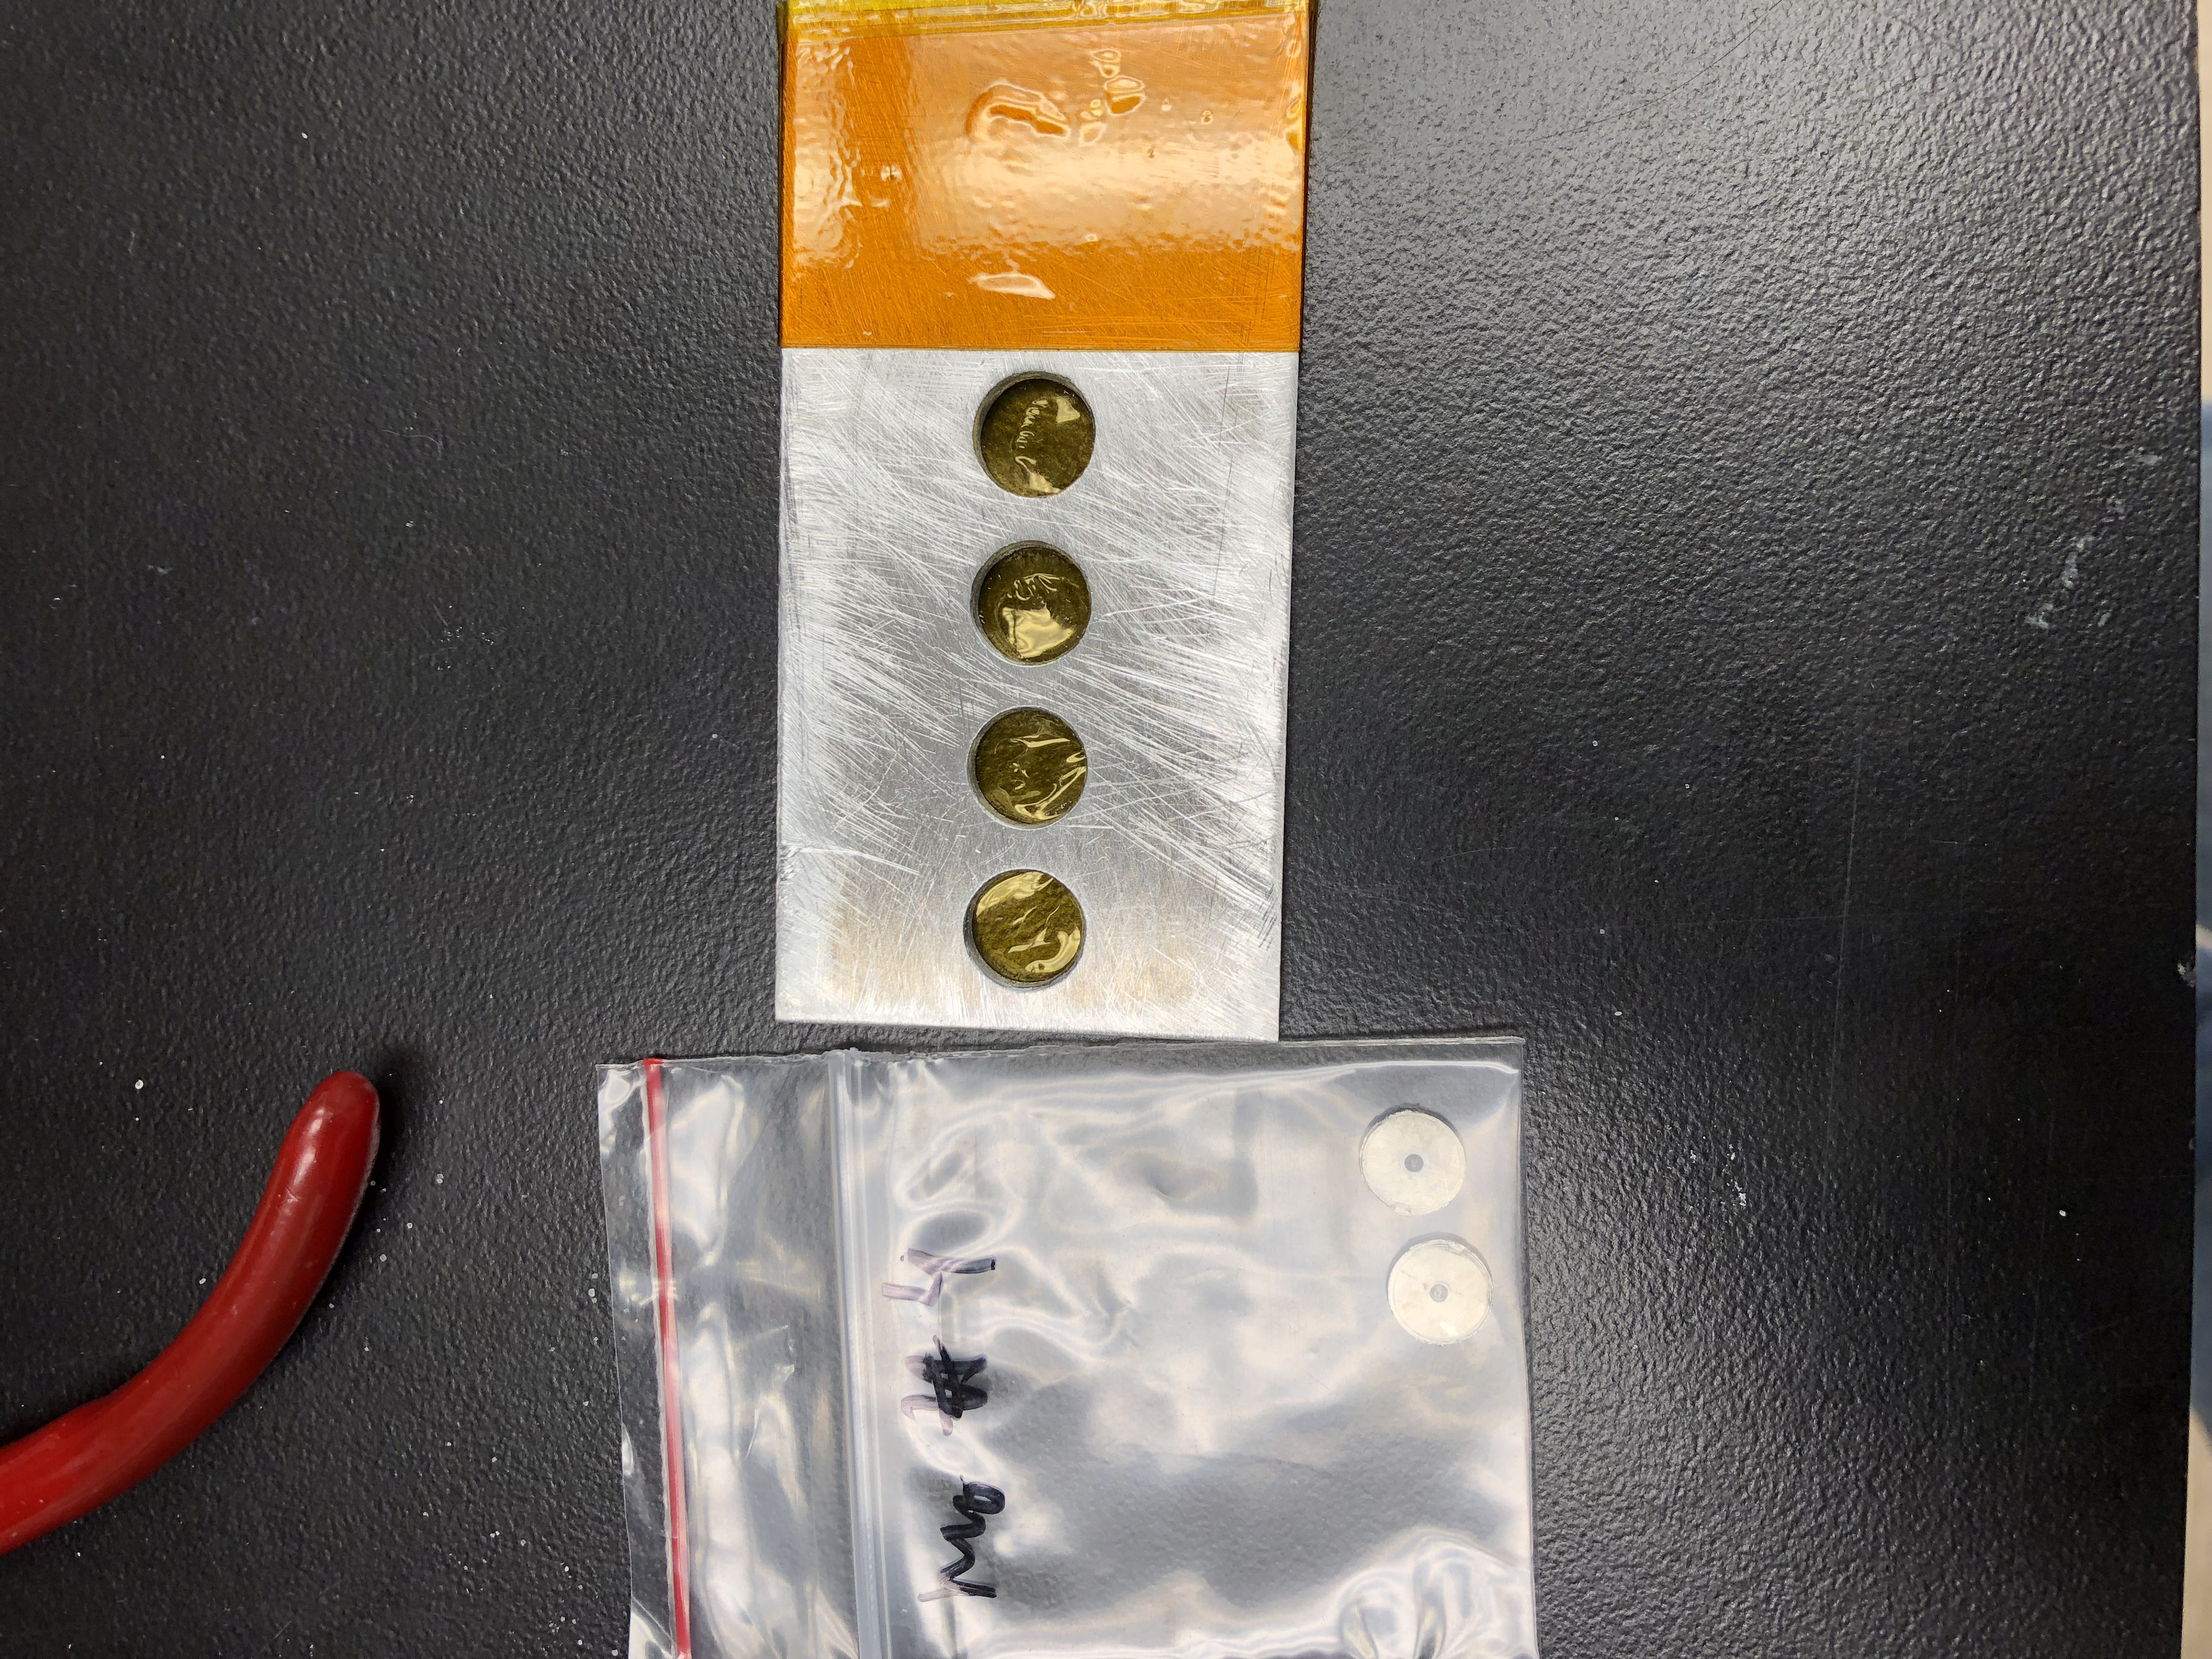
\includegraphics[clip=true,trim=5pt 1000pt 10pt 900pt,width=0.75\columnwidth,angle=90]{./figures/IMG_8840.JPG}
%  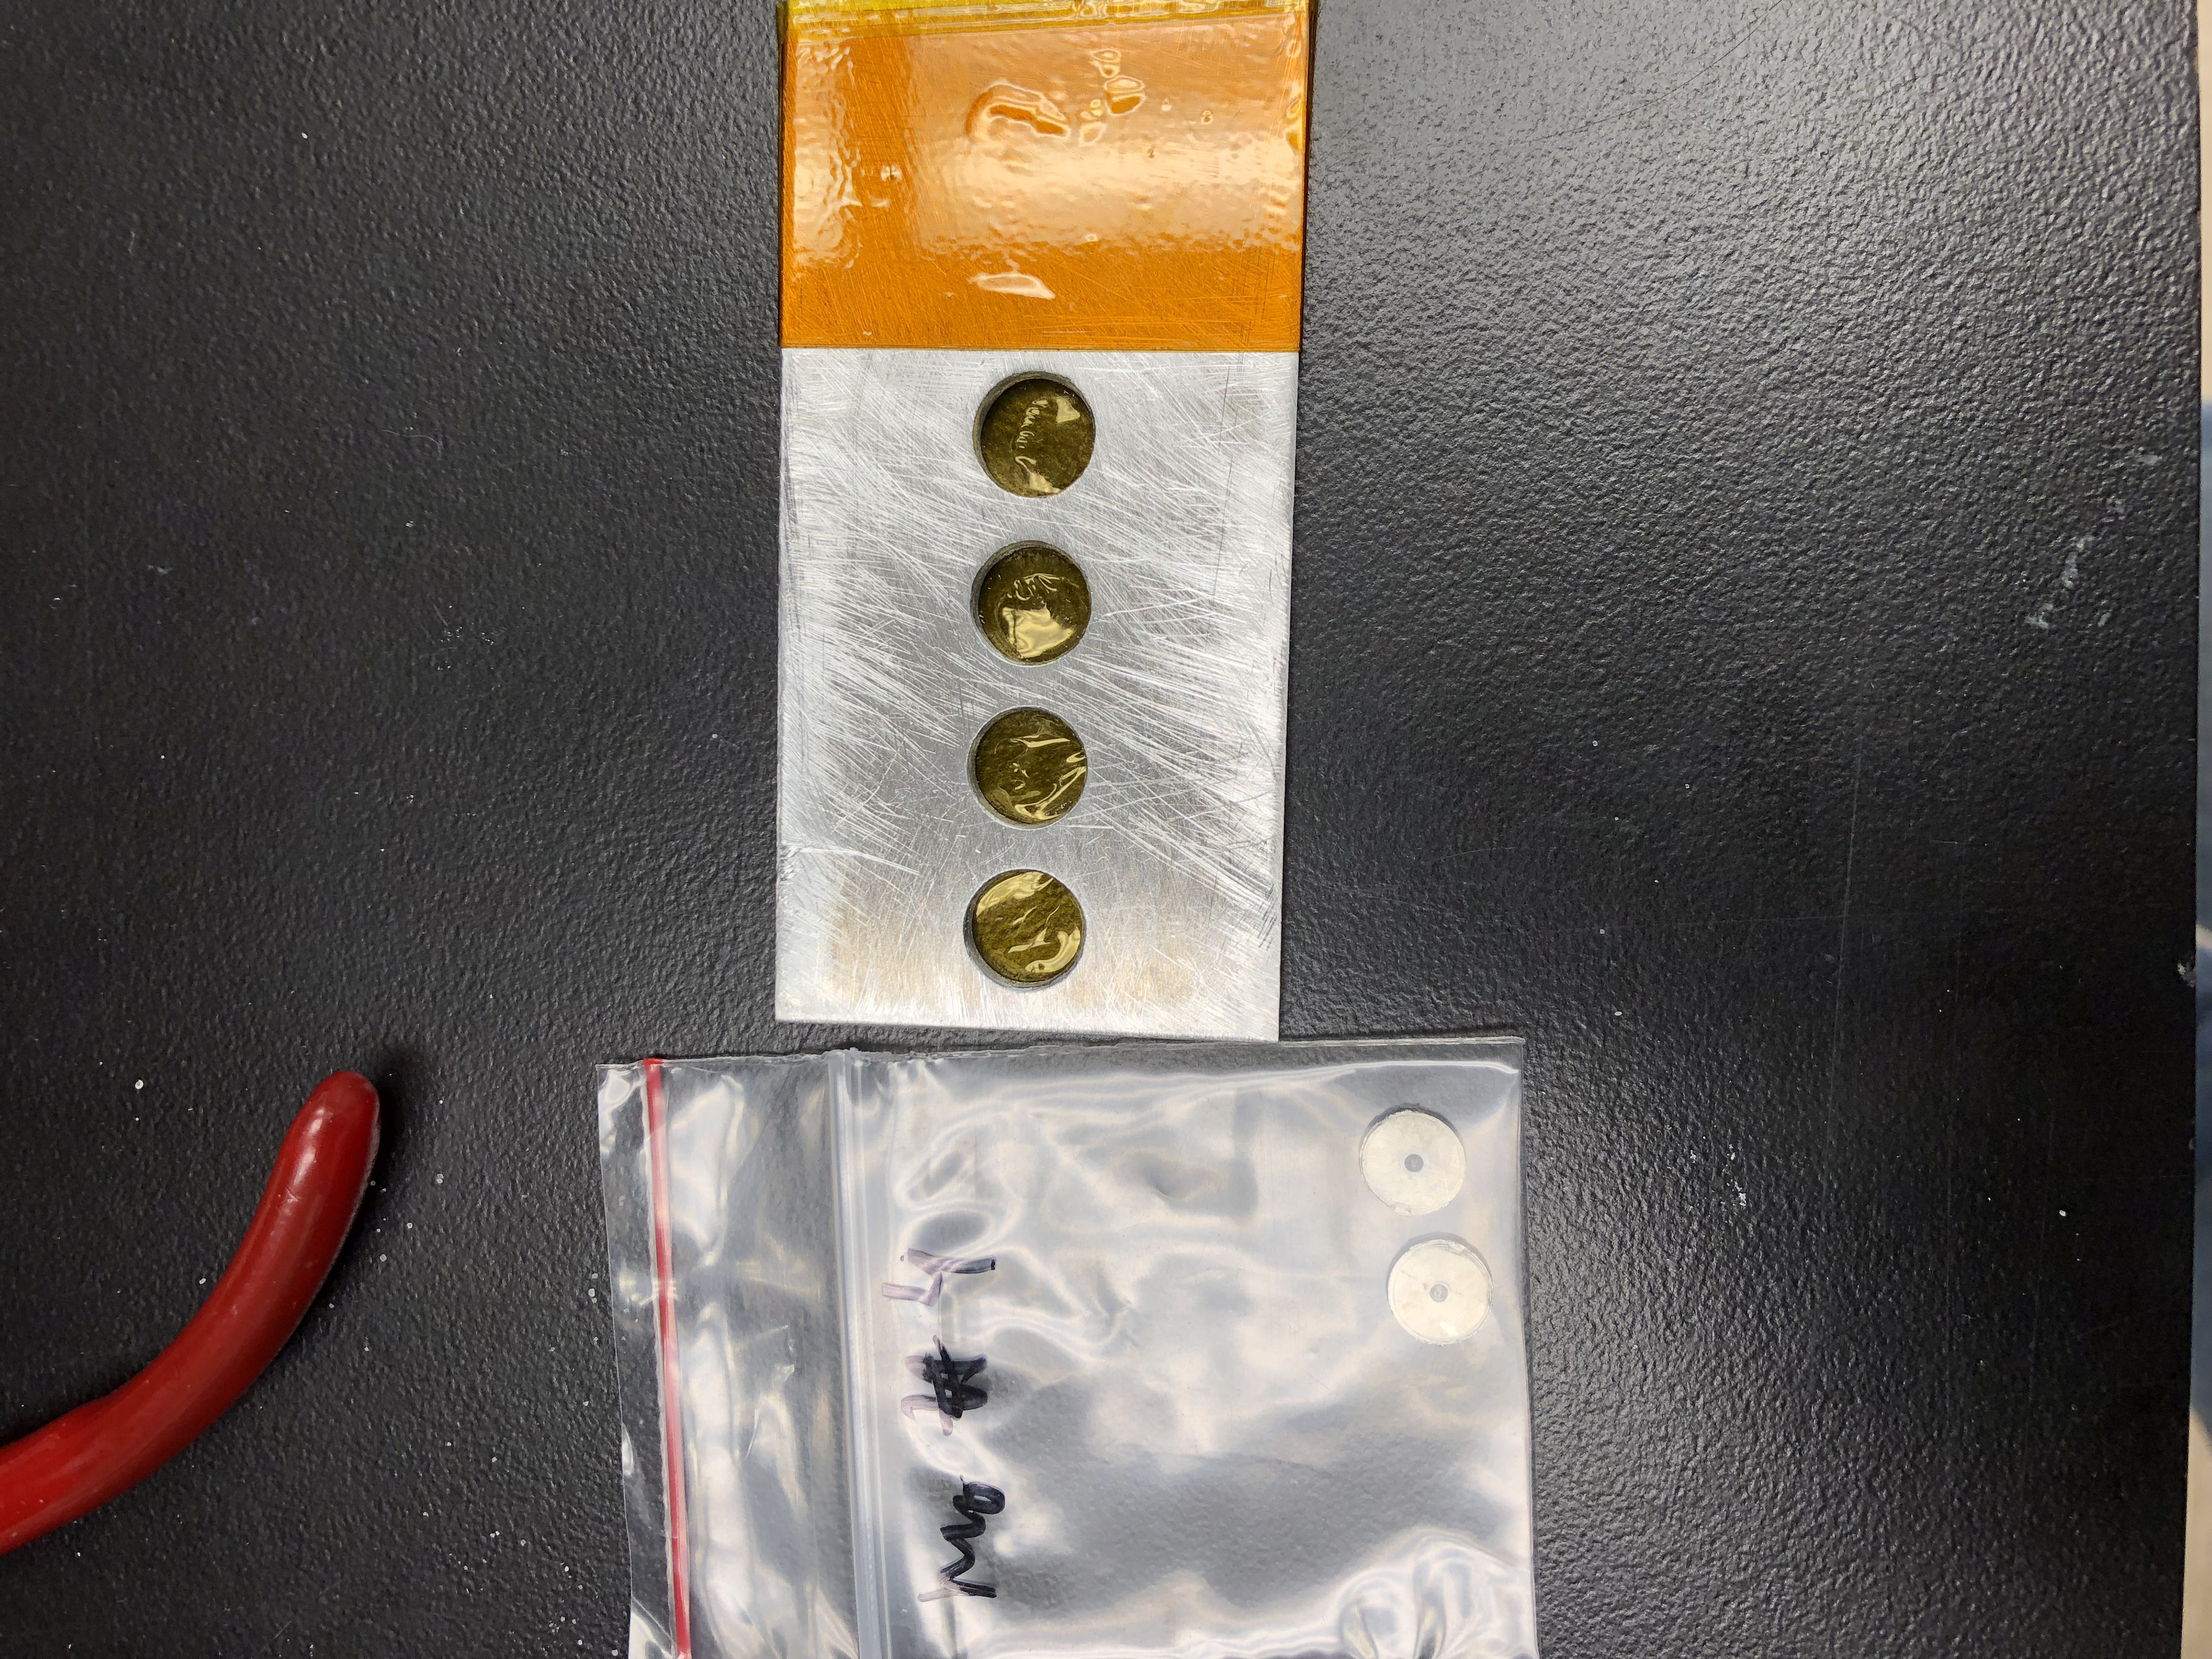
\includegraphics[width=0.75\columnwidth,angle=270]{./figures/IMG_8840.JPG}
 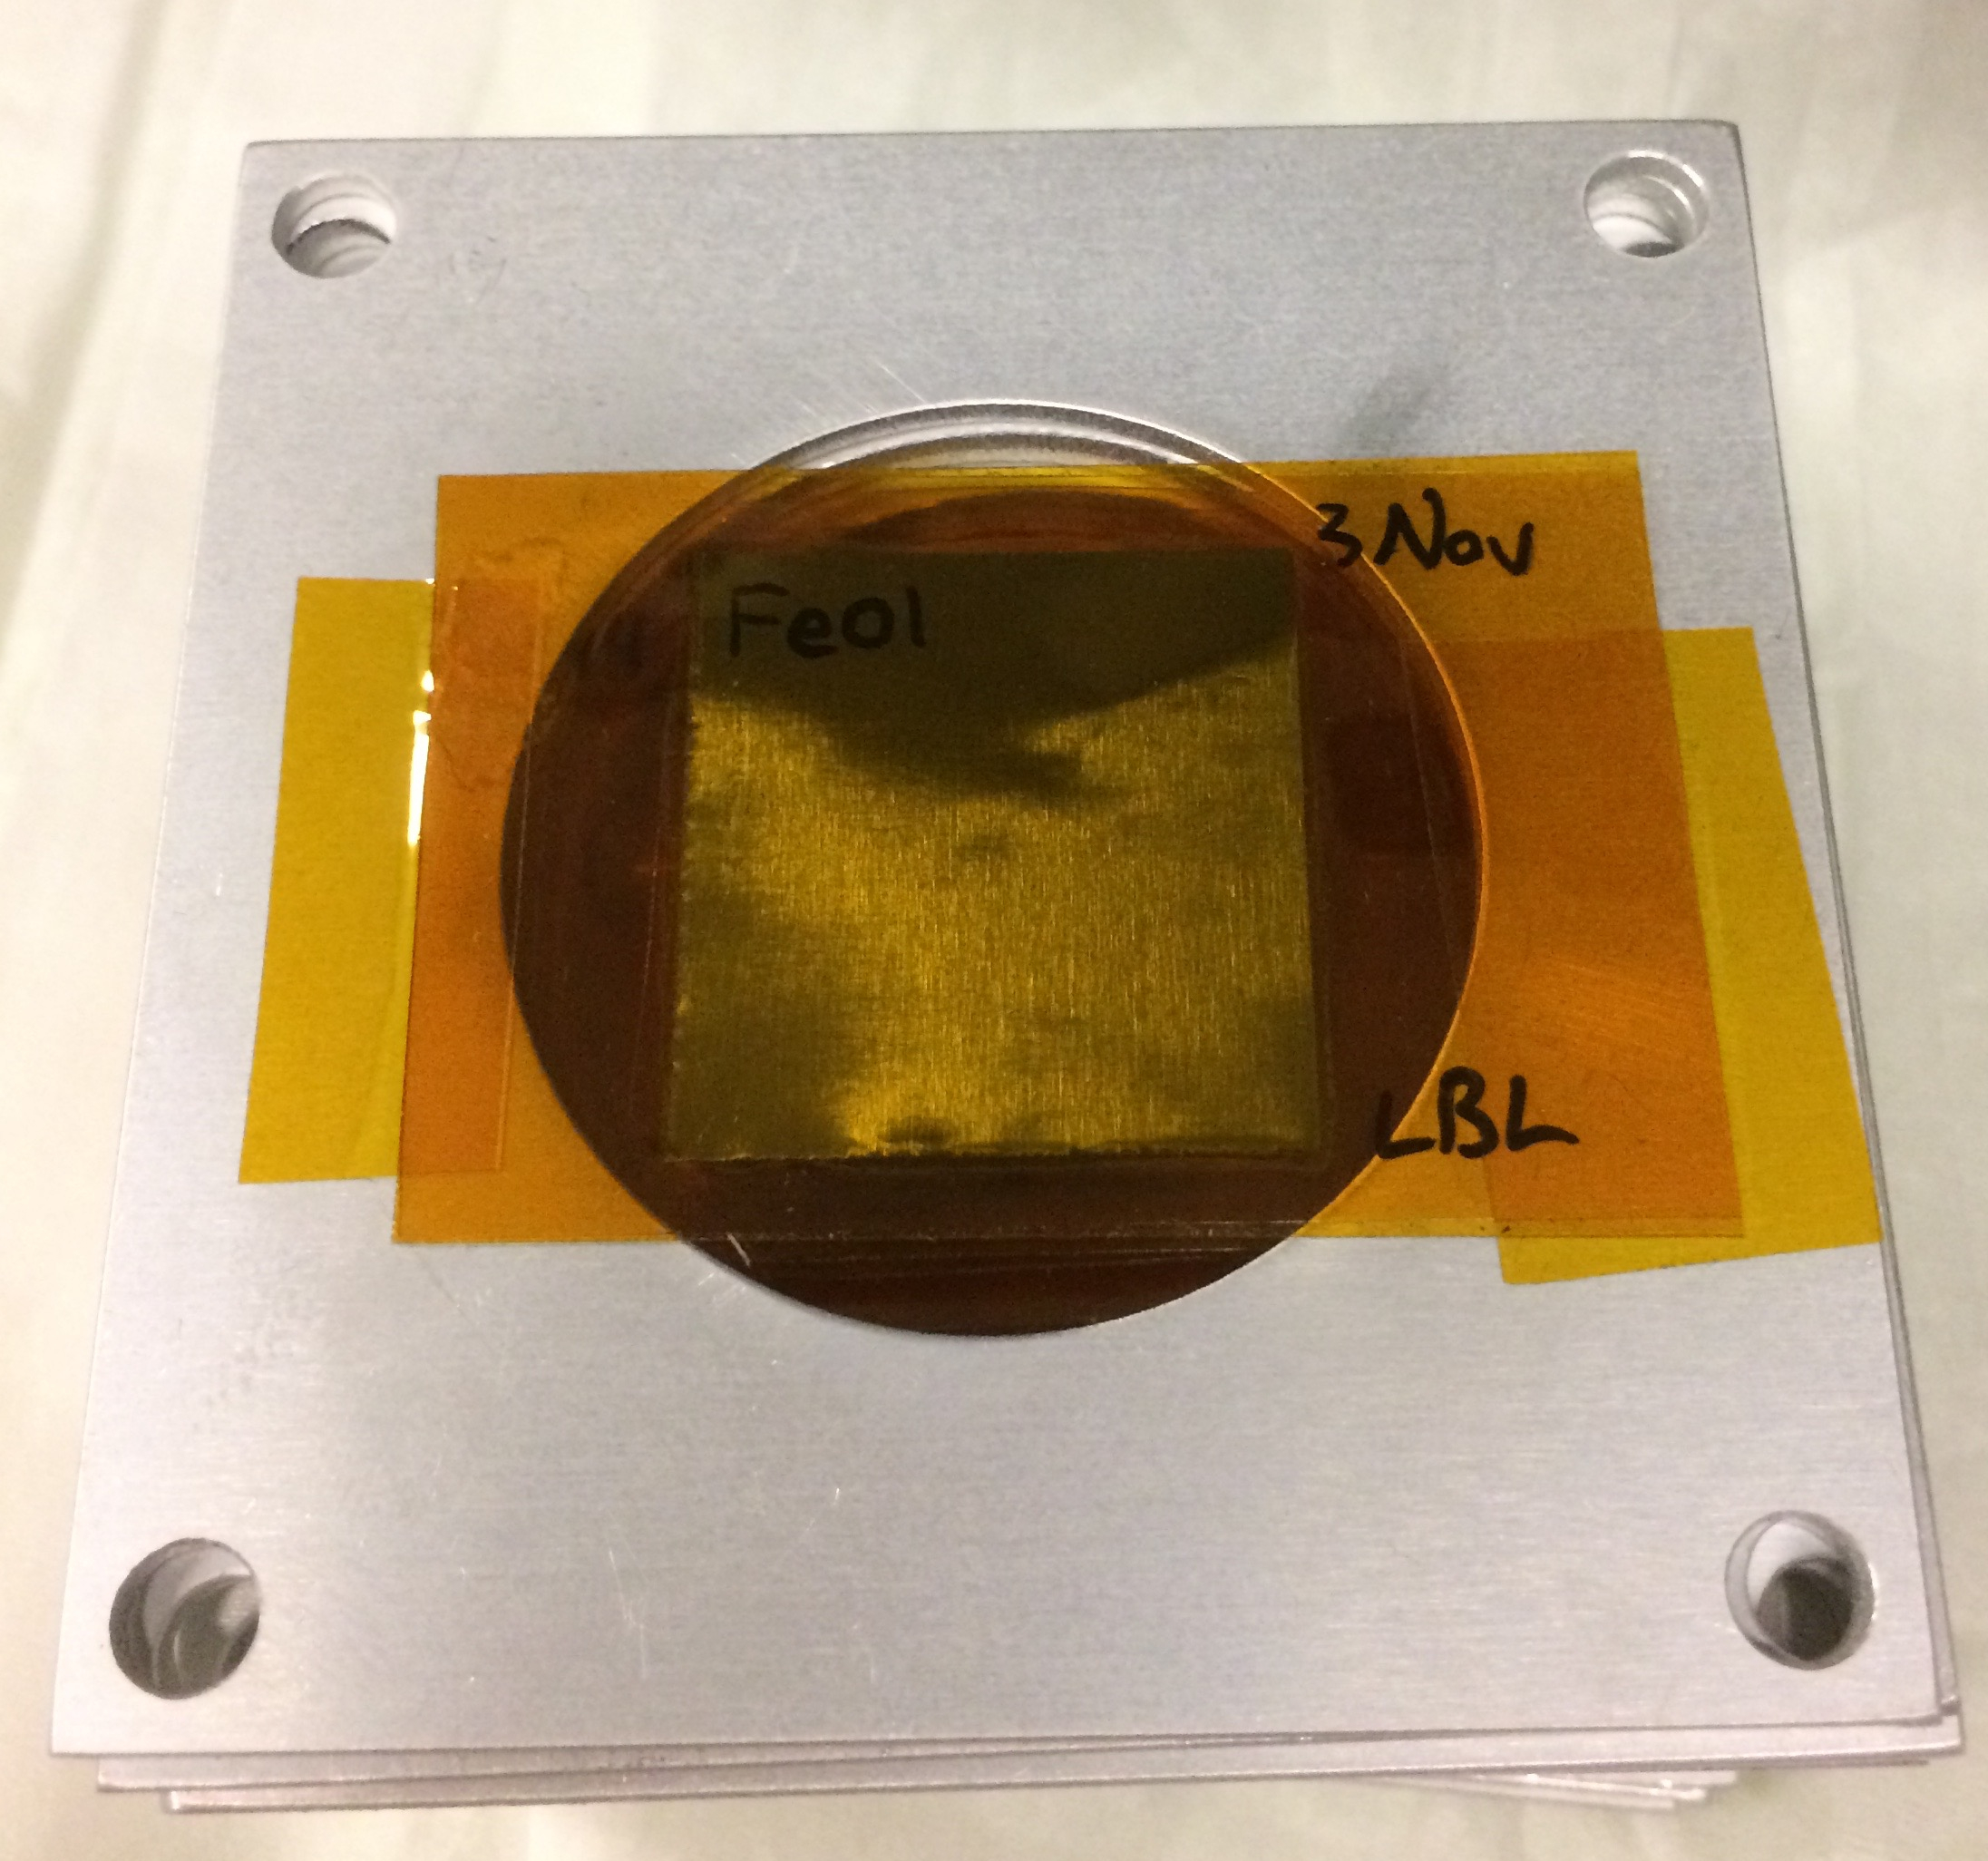
\includegraphics[width=0.5\columnwidth]{./figures/IMG_0305.jpg}
 % IMG_8840.JPG: 4032x3024 pixel, 72dpi, 142.24x106.68 cm, bb=0 0 4032 3024
 \caption{A stack of Fe, Cu, and Ti foils mounted on aluminum frames (Fe-01 visible on top), for the 55\,MeV Fe(p,x) target stack. All foils are mounted over the aperture of a 1.5875 mm-thick aluminum frame.}
 \label{fig:fe_IMG_0305}
\end{figure}



\begin{figure}
 \centering
%                                l   b      r    top
%  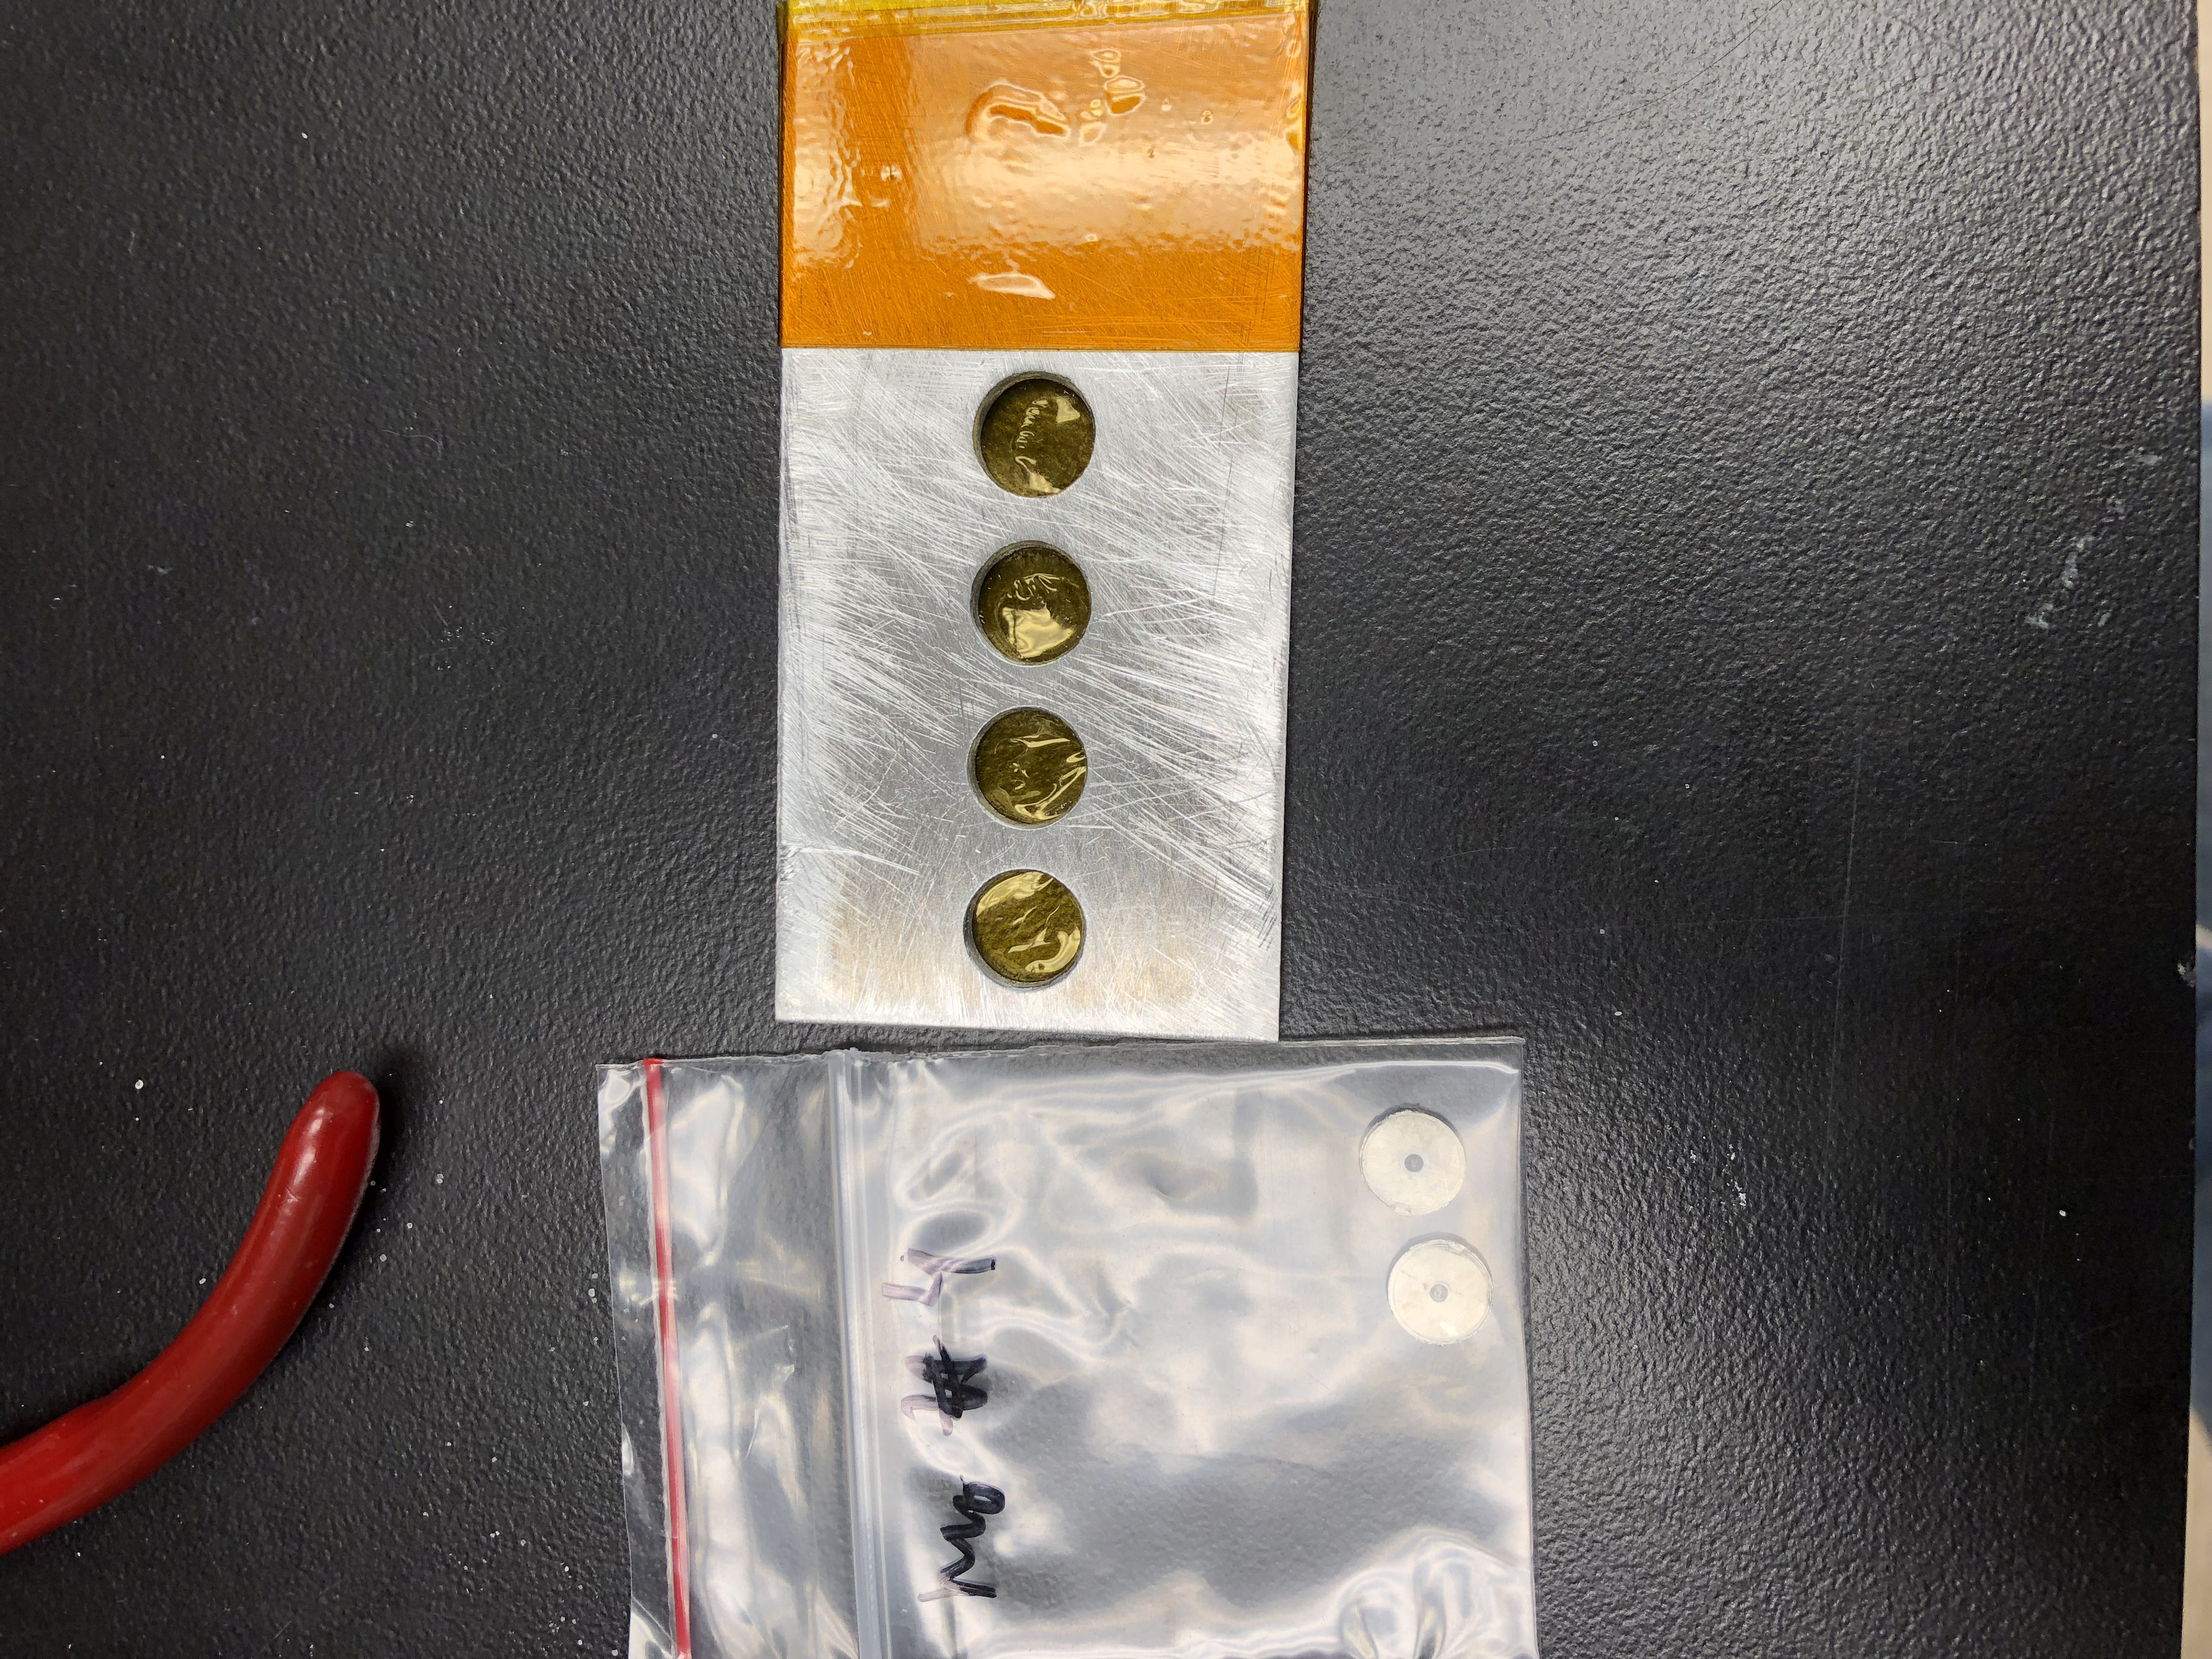
\includegraphics[clip=true,trim=5pt 1000pt 10pt 900pt,width=0.75\columnwidth,angle=90]{./figures/IMG_8840.JPG}
%  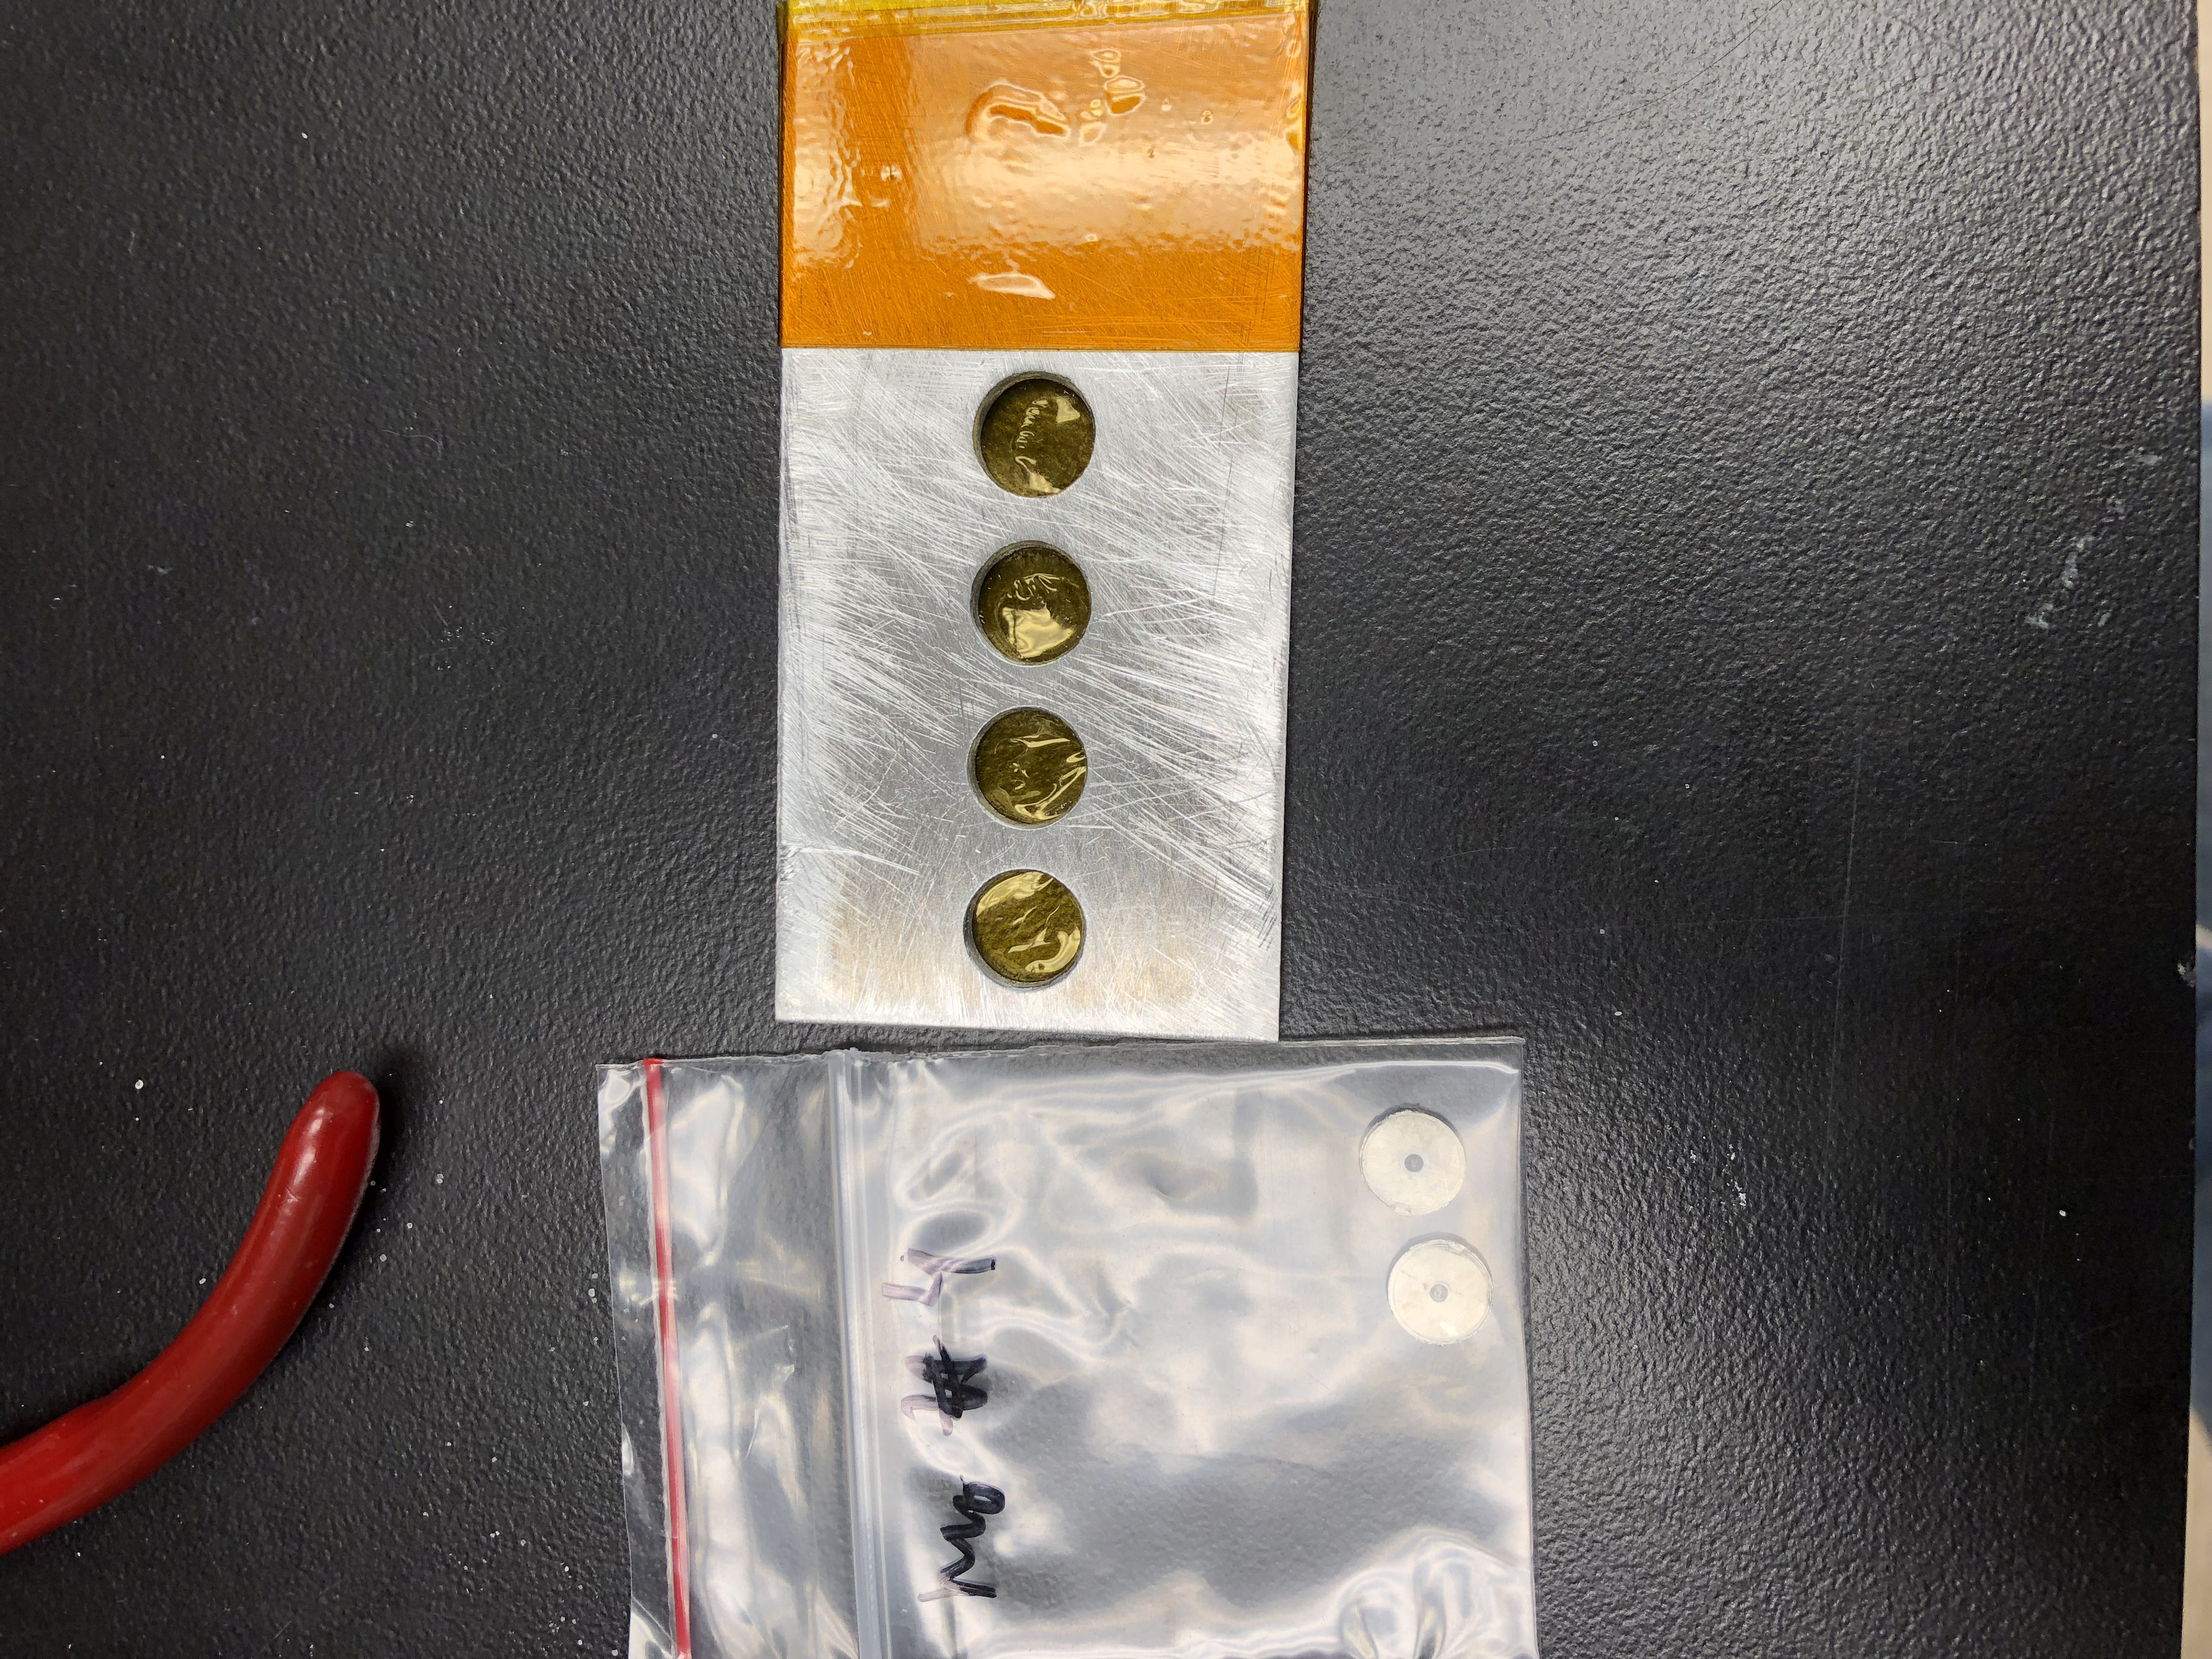
\includegraphics[width=0.75\columnwidth,angle=270]{./figures/IMG_8840.JPG}
 \includegraphics[width=0.75\columnwidth]{./figures/SAM_252_Cu14.JPG}
 % IMG_8840.JPG: 4032x3024 pixel, 72dpi, 142.24x106.68 cm, bb=0 0 4032 3024
 \caption{The ORTEC GMX Series (model \#GMX-50220-S)  High-Purity Germanium detector used for gamma spectroscopy of the activated foils, as described in \autoref{sec:spectroscopy_fe}. The detector, counting foil Cu-14 in this figure, has a \enquote{ladder} permitting counting at various fixed distances (in 1\,cm inetrvals) from the front face of the detector. With the lead shielding lid closed (for reduced background), the ladder permits counting up to 18\,cm, and up to 75\,cm with the lid open.   }
 \label{fig:fe_IMG_1984}
\end{figure}



\subsubsection{MCNP modeling}



% 
% Update description of both of the simulation pictures here
% 
%
A rendering of the 55\,MeV Fe(p,x) target stack, as modeled in MCNP6, is seen in \autoref{fig:fe_vised_55}.
% This figure presents a small subset of the full MCNP6 model of the HFNG,  to better illustrate the geometry of the target chamber.
This model is the same described in \autoref{sec:proton_transport_fe} for simulation of proton transport.
The full input file for this MCNP model is included here for reference, in Appendix \ref{sec:88_mcnp_deck}.
In this figure, the 55\,MeV proton beam enters from the left of the figure, where it is incident (in the positive $x$ direction) upon the SS-3 profile monitor.
The other stack elements, described in  \autoref{tab:fe_stack_table} are illustrated here, as well.
% 
% Add this back in after updating
% 
% \textred{The green cell is the cooling water channel for the target box, the air filling the target box is shown in light blue, and the 6061 aluminum beam degraders are shown in dark blue.  
% The thin black lines seen in between degraders are the Nb, Cu, and Al activation points at each energy position, sealed in Kapton tape. }
The detail of each foil sealed in the Kapton is not visible here, simply due to the size scale of the stack assembly.
Similarly, a rendering of the 25\,MeV Fe(p,x) target stack, as modeled in MCNP6, is seen in \autoref{fig:fe_vised_25}.
% This figure presents a small subset of the full MCNP6 model of the HFNG,  to better illustrate the geometry of the target chamber.
% This model is the same described in \autoref{sec:proton_transport_fe} for simulation of proton transport.
The full input file for this MCNP model is included here for reference, in Appendix \ref{sec:88_mcnp_deck_lowE}.




% 
% Update the descriptions of tehse figures
% 
%

\begin{figure}
 \centering
 %trim option's parameter order: left bottom right top
 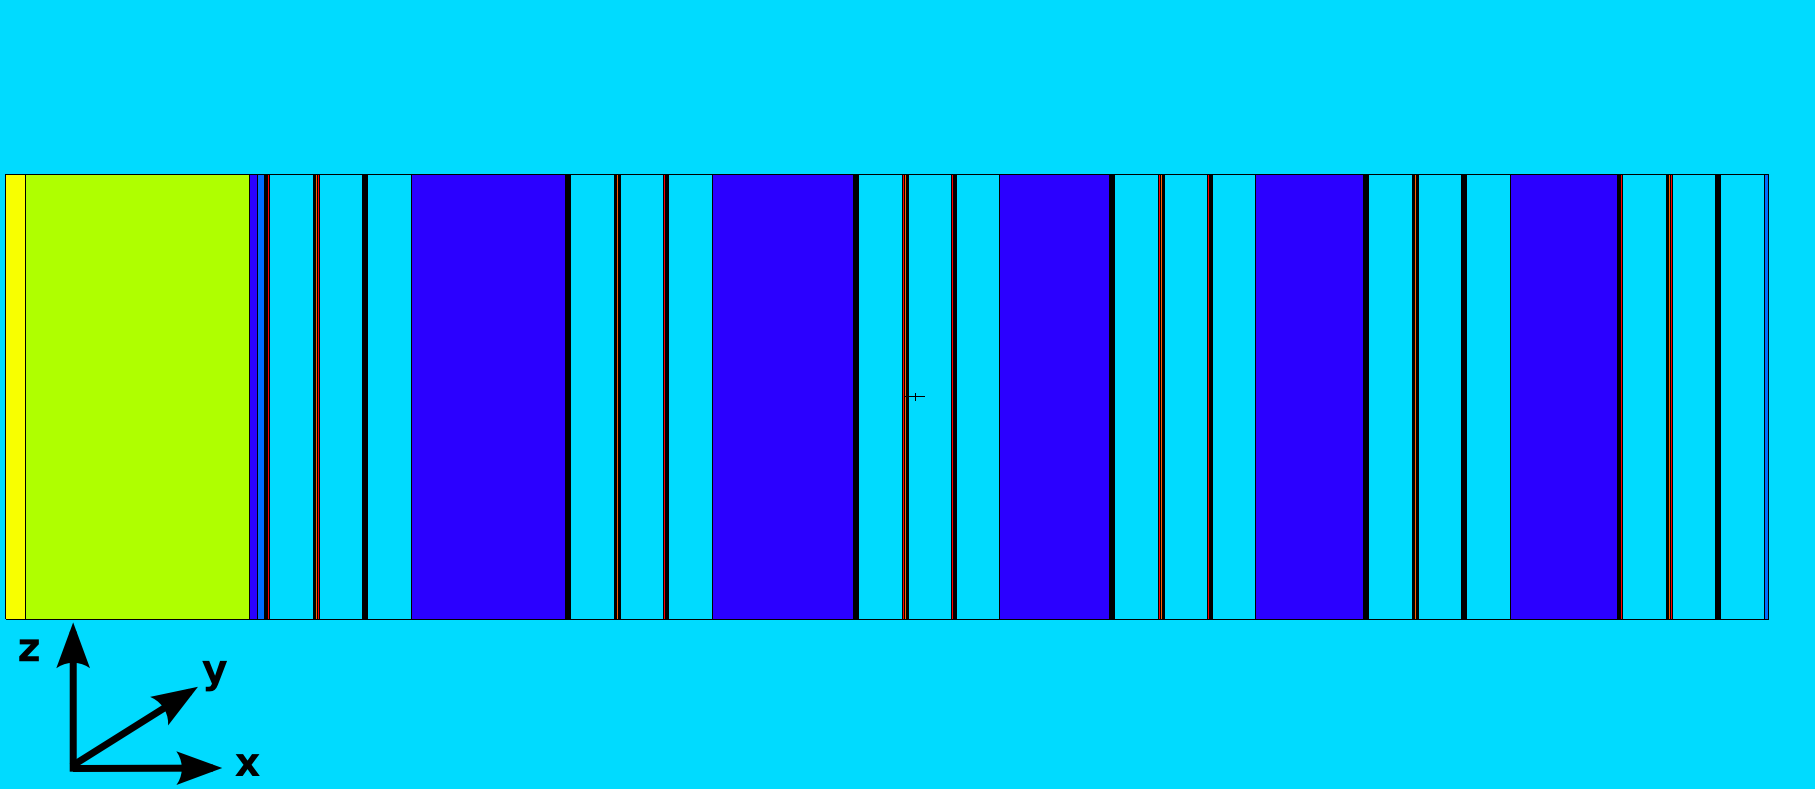
\includegraphics[trim = 0mm 0mm 2mm 0mm, clip,width=0.75\columnwidth]{./figures/ipf_stack_nolabels_axes.PNG}
 % mcnp_vised2.PNG.png: 688x443 pixel, 96dpi, 18.21x11.72 cm, bb=0 0 516 332
%   \caption{Simplified top-down MCNP6 model of the IPF Nb(p,x) target stack. The 100\,MeV proton beam enters from the left of the figure, where it is incident upon the Inconel beam entrance window (yellow). The beam is transported down the length of the stack, towards the rear of the stack on the right side of the figure.
 \caption{Simplified top-down MCNP6 model of the 55\,MeV Fe(p,x) target stack. The  proton beam enters from the left of the figure, where it is incident upon the SS-3 profile monitor. The beam is transported down the length of the stack, towards the rear of the stack on the right side of the figure.
%  MCNP6 model of the HFNG target chamber, with reference scale. The co-loaded foils can be seen in the target chamber center.  The ovals indicate the location of water cooling channels.
}
 \label{fig:fe_vised_55}
\end{figure}


\begin{figure}
 \centering
 %trim option's parameter order: left bottom right top
 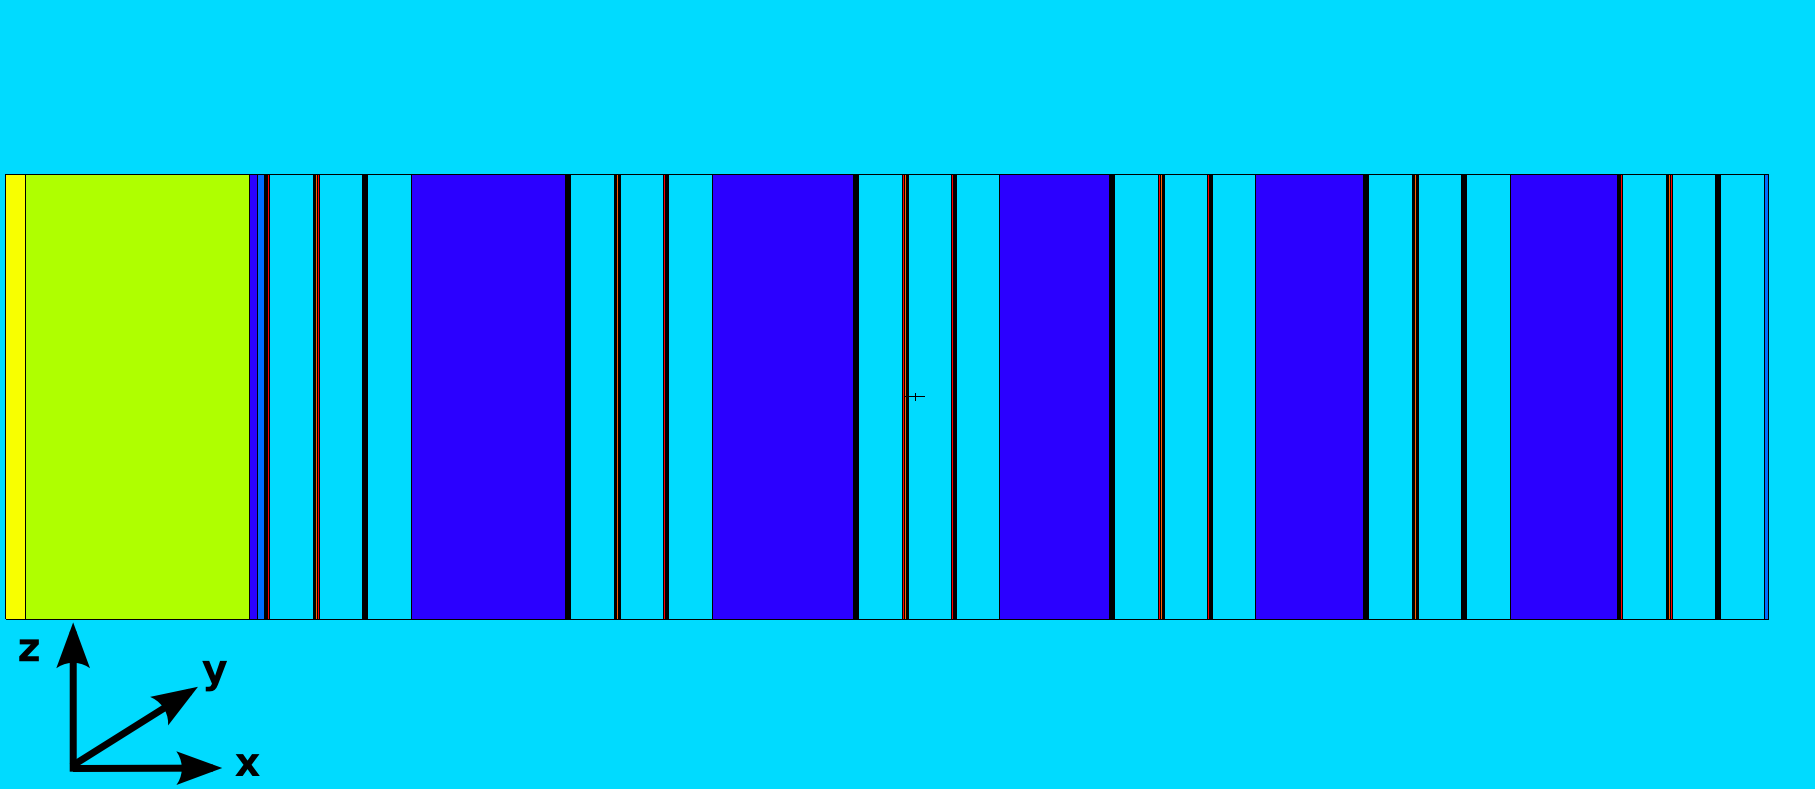
\includegraphics[trim = 0mm 0mm 2mm 0mm, clip,width=0.75\columnwidth]{./figures/ipf_stack_nolabels_axes.PNG}
 % mcnp_vised2.PNG.png: 688x443 pixel, 96dpi, 18.21x11.72 cm, bb=0 0 516 332
%   \caption{Simplified top-down MCNP6 model of the IPF Nb(p,x) target stack. The 100\,MeV proton beam enters from the left of the figure, where it is incident upon the Inconel beam entrance window (yellow). The beam is transported down the length of the stack, towards the rear of the stack on the right side of the figure.
\caption{Simplified top-down MCNP6 model of the 25\,MeV  Fe(p,x) target stack. The  proton beam enters from the left of the figure, where it is incident upon the SS-5 profile monitor. The beam is transported down the length of the stack, towards the rear of the stack on the right side of the figure.
%  MCNP6 model of the HFNG target chamber, with reference scale. The co-loaded foils can be seen in the target chamber center.  The ovals indicate the location of water cooling channels.
}
 \label{fig:fe_vised_25}
\end{figure}




% 
% Removed, since I didnt finish the analysis
% 
% 
% 

% \begin{figure*}
%     \centering    
%     \subfloat{
%         \centering
% %         \includegraphics[width=\textwidth]{./figures/target2.png}
%         \subfigimg[width=0.495\textwidth]{a)}{./figures/Al_ptallies.pdf}{80}
% %         \caption{Decay curve for the $\beta^-$ decay of \ce{^{116}In}.}
%         %         \refstepcounter{subfigure}
% %          \label{fig:91mNb}
% %    }
% %      \subfloat{
% %         \centering
% %         \includegraphics[width=\columnwidth]{./figures/Capture.PNG}
%         \subfigimg[width=0.495\textwidth]{b)}{./figures/Cu_ptallies.pdf}{80}
% %         \caption{ Decay curve for the $\beta^+$ decay of \ce{^{64}Cu}.}
% %         \refstepcounter{subfigure} 
% %         \label{fig:92mNb}
%    \hspace{-10pt}}%
%     \caption{\textred{Update this figure!!!} Final variance minimized incident proton energy distributions for the (a) Cu and (b) Ti foils, as simulated in MCNP6. The distribution tallies in each foil are all normalized to be per source proton, which was $10^8$ in all simulations. As the beam is degraded, proton energy distributions become visibly broadened due to straggling, and drop in magnitude due to scattering losses.}
% %      \phantomcaption{}
%      \label{fig:fe_ptallies_appendix}
% \end{figure*}


% Using this MCNP6 model, the proton energy distribution is tallied in all volumes of the stack assembly.
% As seen in \autoref{fig:Fe_ptallies} of \autoref{sec:proton_transport_fe}, the corresponding incident proton  energy distributions $\frac{d\phi}{dE}$ from MCNP6 simulation (using the variance minimized degrader density) are shown for the six irradiated Cu and Ti  foils in \autoref{fig:fe_ptallies_appendix}. 
% In addition, the MCNP6 model tracks the production and transport of secondary neutrons produced through (p,xn) reactions on the target stack components.
% The the proton energy distribution is tallied in all Ti, Cu, and Fe foils, and is seen in \autoref{fig:fe_ntallies}. 
% The neutron flux is consistently 3--4 orders of magnitude smaller than the corresponding proton flux, and is seen to be visibly  downscattered when moving down the stack.
% 
% \begin{figure*}
%     \centering    
%     \subfloat{
%         \centering
% %         \includegraphics[width=\textwidth]{./figures/target2.png}
%         \subfigimg[width=0.497\textwidth]{a)}{./figures/Al_ntallies.pdf}{50}
% %         \caption{Decay curve for the $\beta^-$ decay of \ce{^{116}In}.}
%         %         \refstepcounter{subfigure}
% %          \label{fig:91mNb}
% %    }
% %      \subfloat{
% %         \centering
% %         \includegraphics[width=\columnwidth]{./figures/Capture.PNG}
%         \subfigimg[width=0.497\textwidth]{b)}{./figures/Cu_ntallies.pdf}{50}
% %         \caption{ Decay curve for the $\beta^+$ decay of \ce{^{64}Cu}.}
% %         \refstepcounter{subfigure} 
% %         \label{fig:92mNb}
%    \hspace{-10pt}}%
%     \\
%     \subfloat{
%         \centering
% %         \includegraphics[width=\columnwidth]{./figures/Capture.PNG}
%         \subfigimg[width=0.497\textwidth]{c)}{./figures/Nb_ntallies.pdf}{50}
% %         \caption{ Decay curve for the isomeric transition of \ce{^{115m}In}.}
% %         \refstepcounter{subfigure}
% %          \label{fig:93mMo}
%    }%
%     \caption{\textred{Update this figure!!!} Final variance minimized incident neutron energy distributions for the (a) Cu, (b) Ti, and (C) Fe foils, as simulated in MCNP6. The distribution tallies in each foil are all normalized to be per source proton, which was $10^8$ in all simulations. As the beam is degraded, neutron energy distributions become visibly downscattered.}
% %      \phantomcaption{}
%      \label{fig:fe_ntallies}
% \end{figure*}
% 
% 
% 
% 
% 
% % \begin{figure}
% %  \centering
% % %                                l   b      r    top
% % %  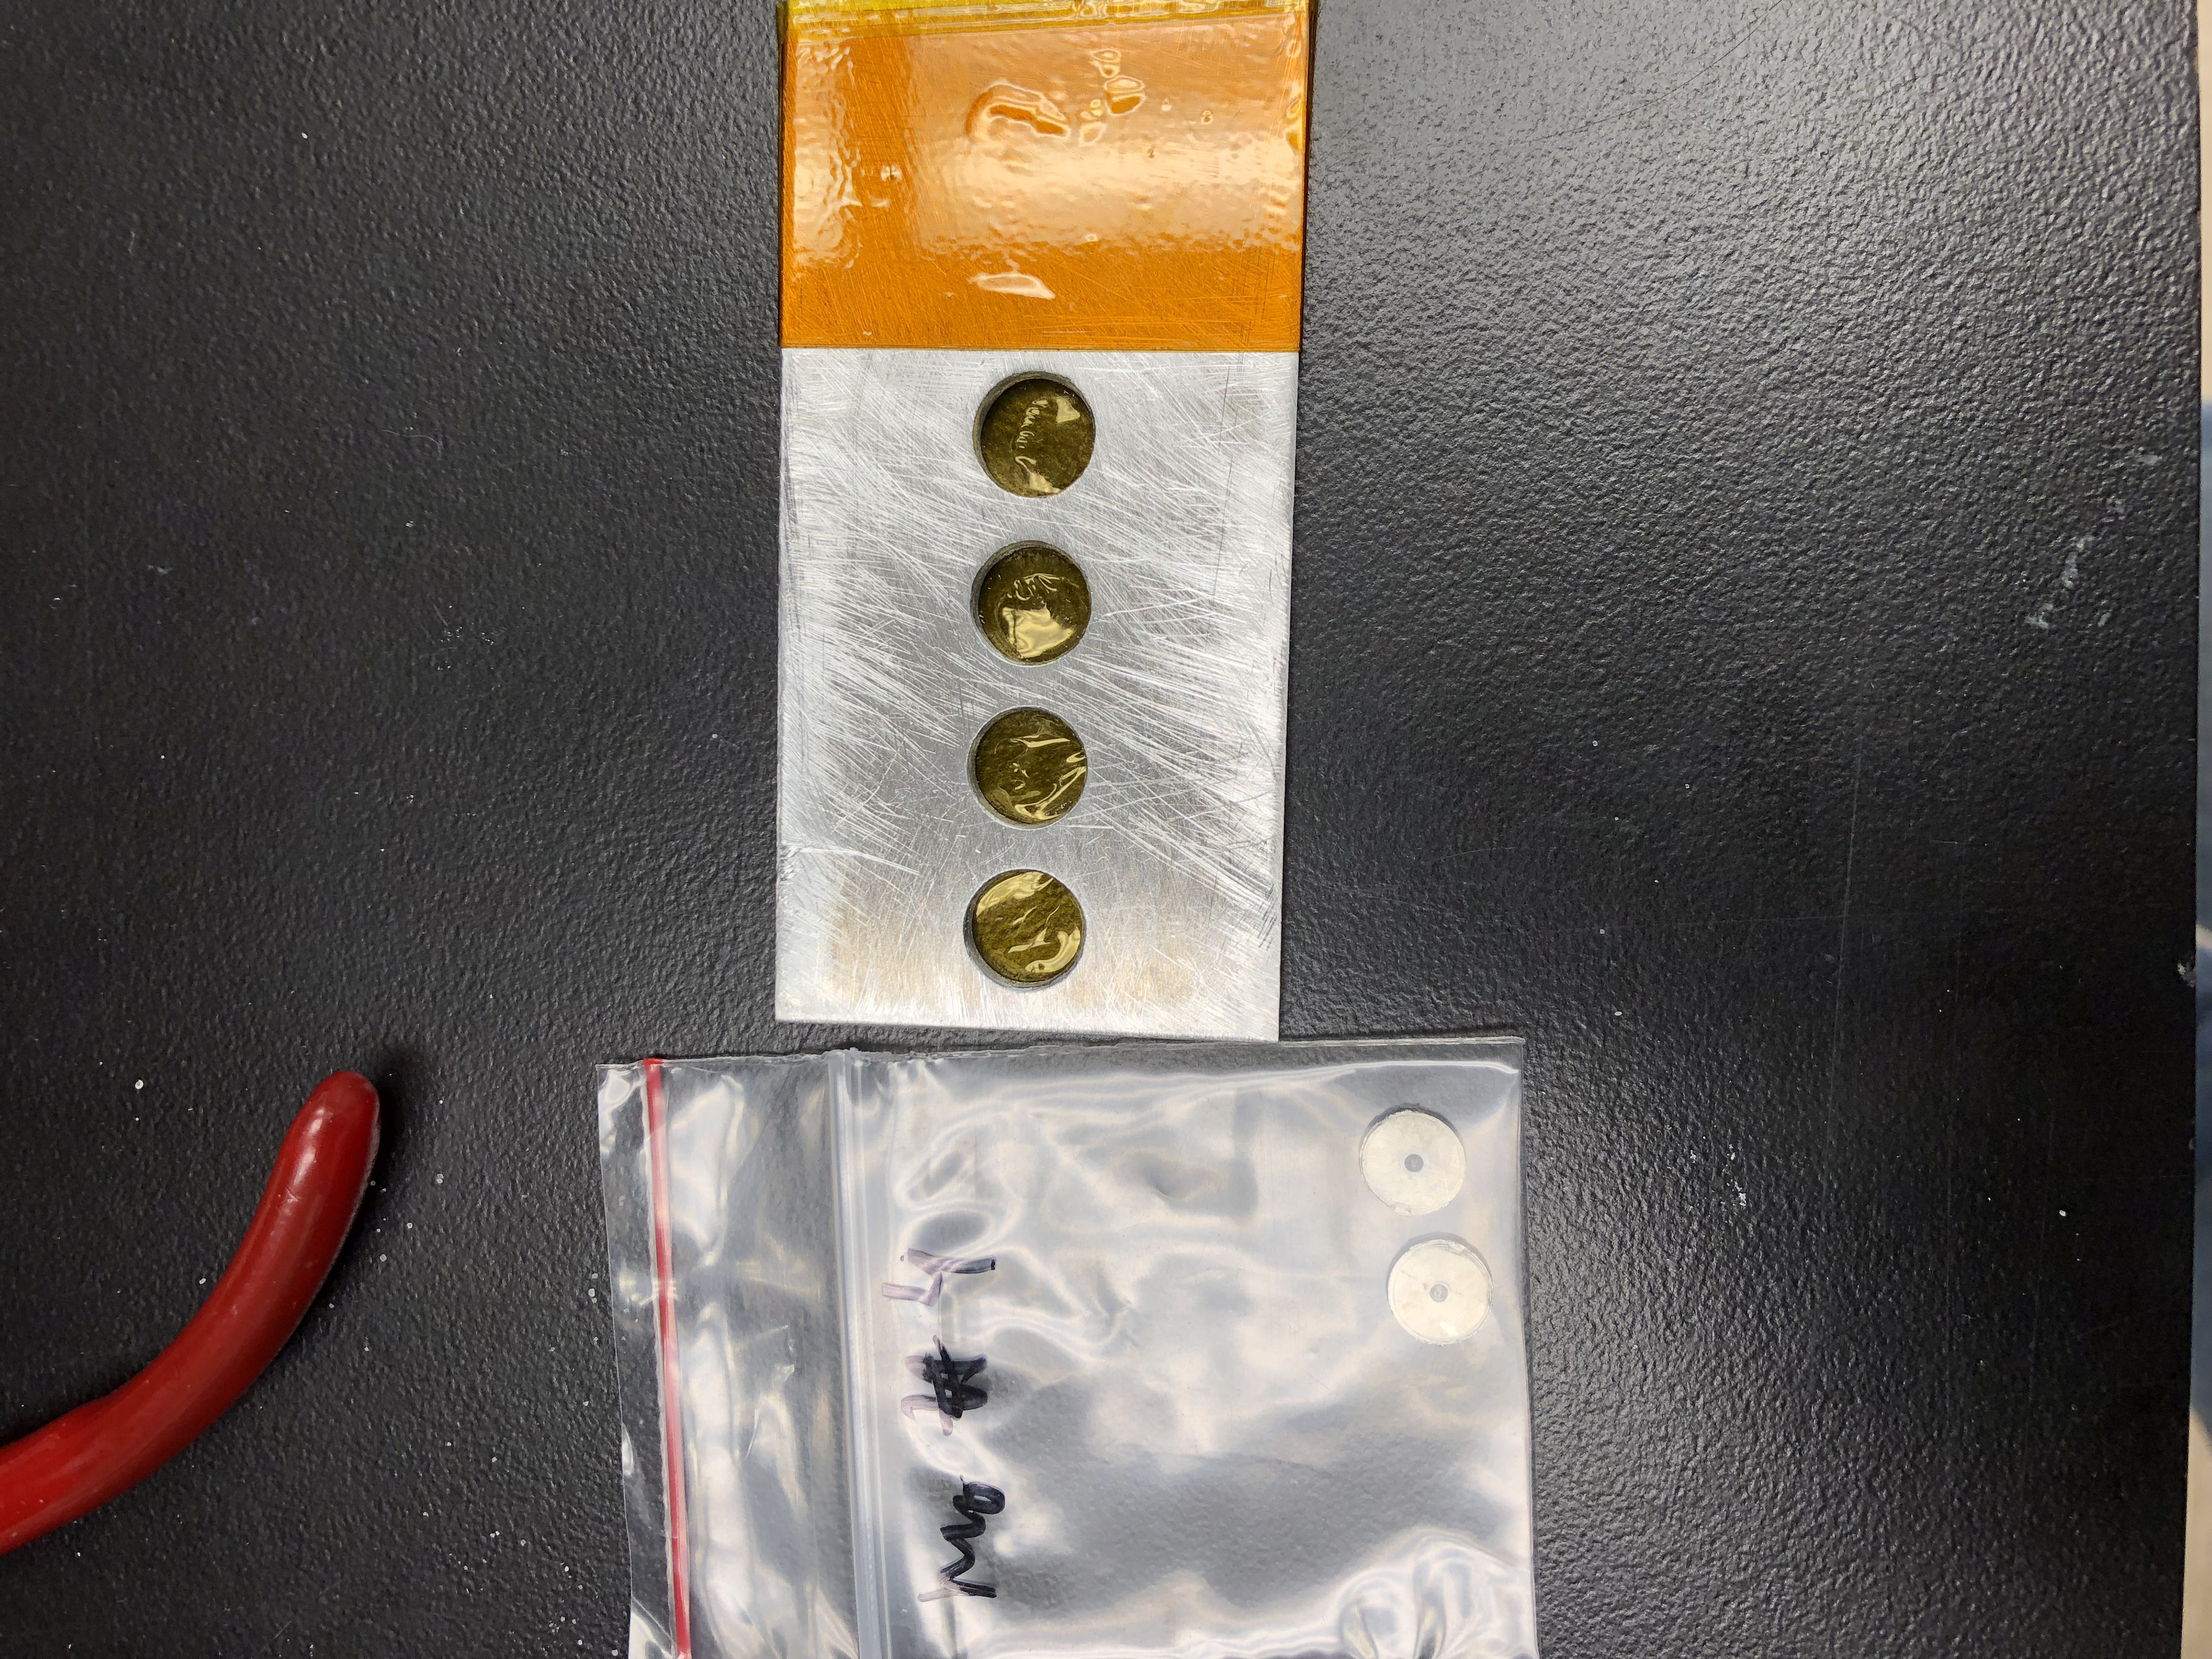
\includegraphics[clip=true,trim=5pt 1000pt 10pt 900pt,width=0.75\columnwidth,angle=90]{./figures/IMG_8840.JPG}
% % %  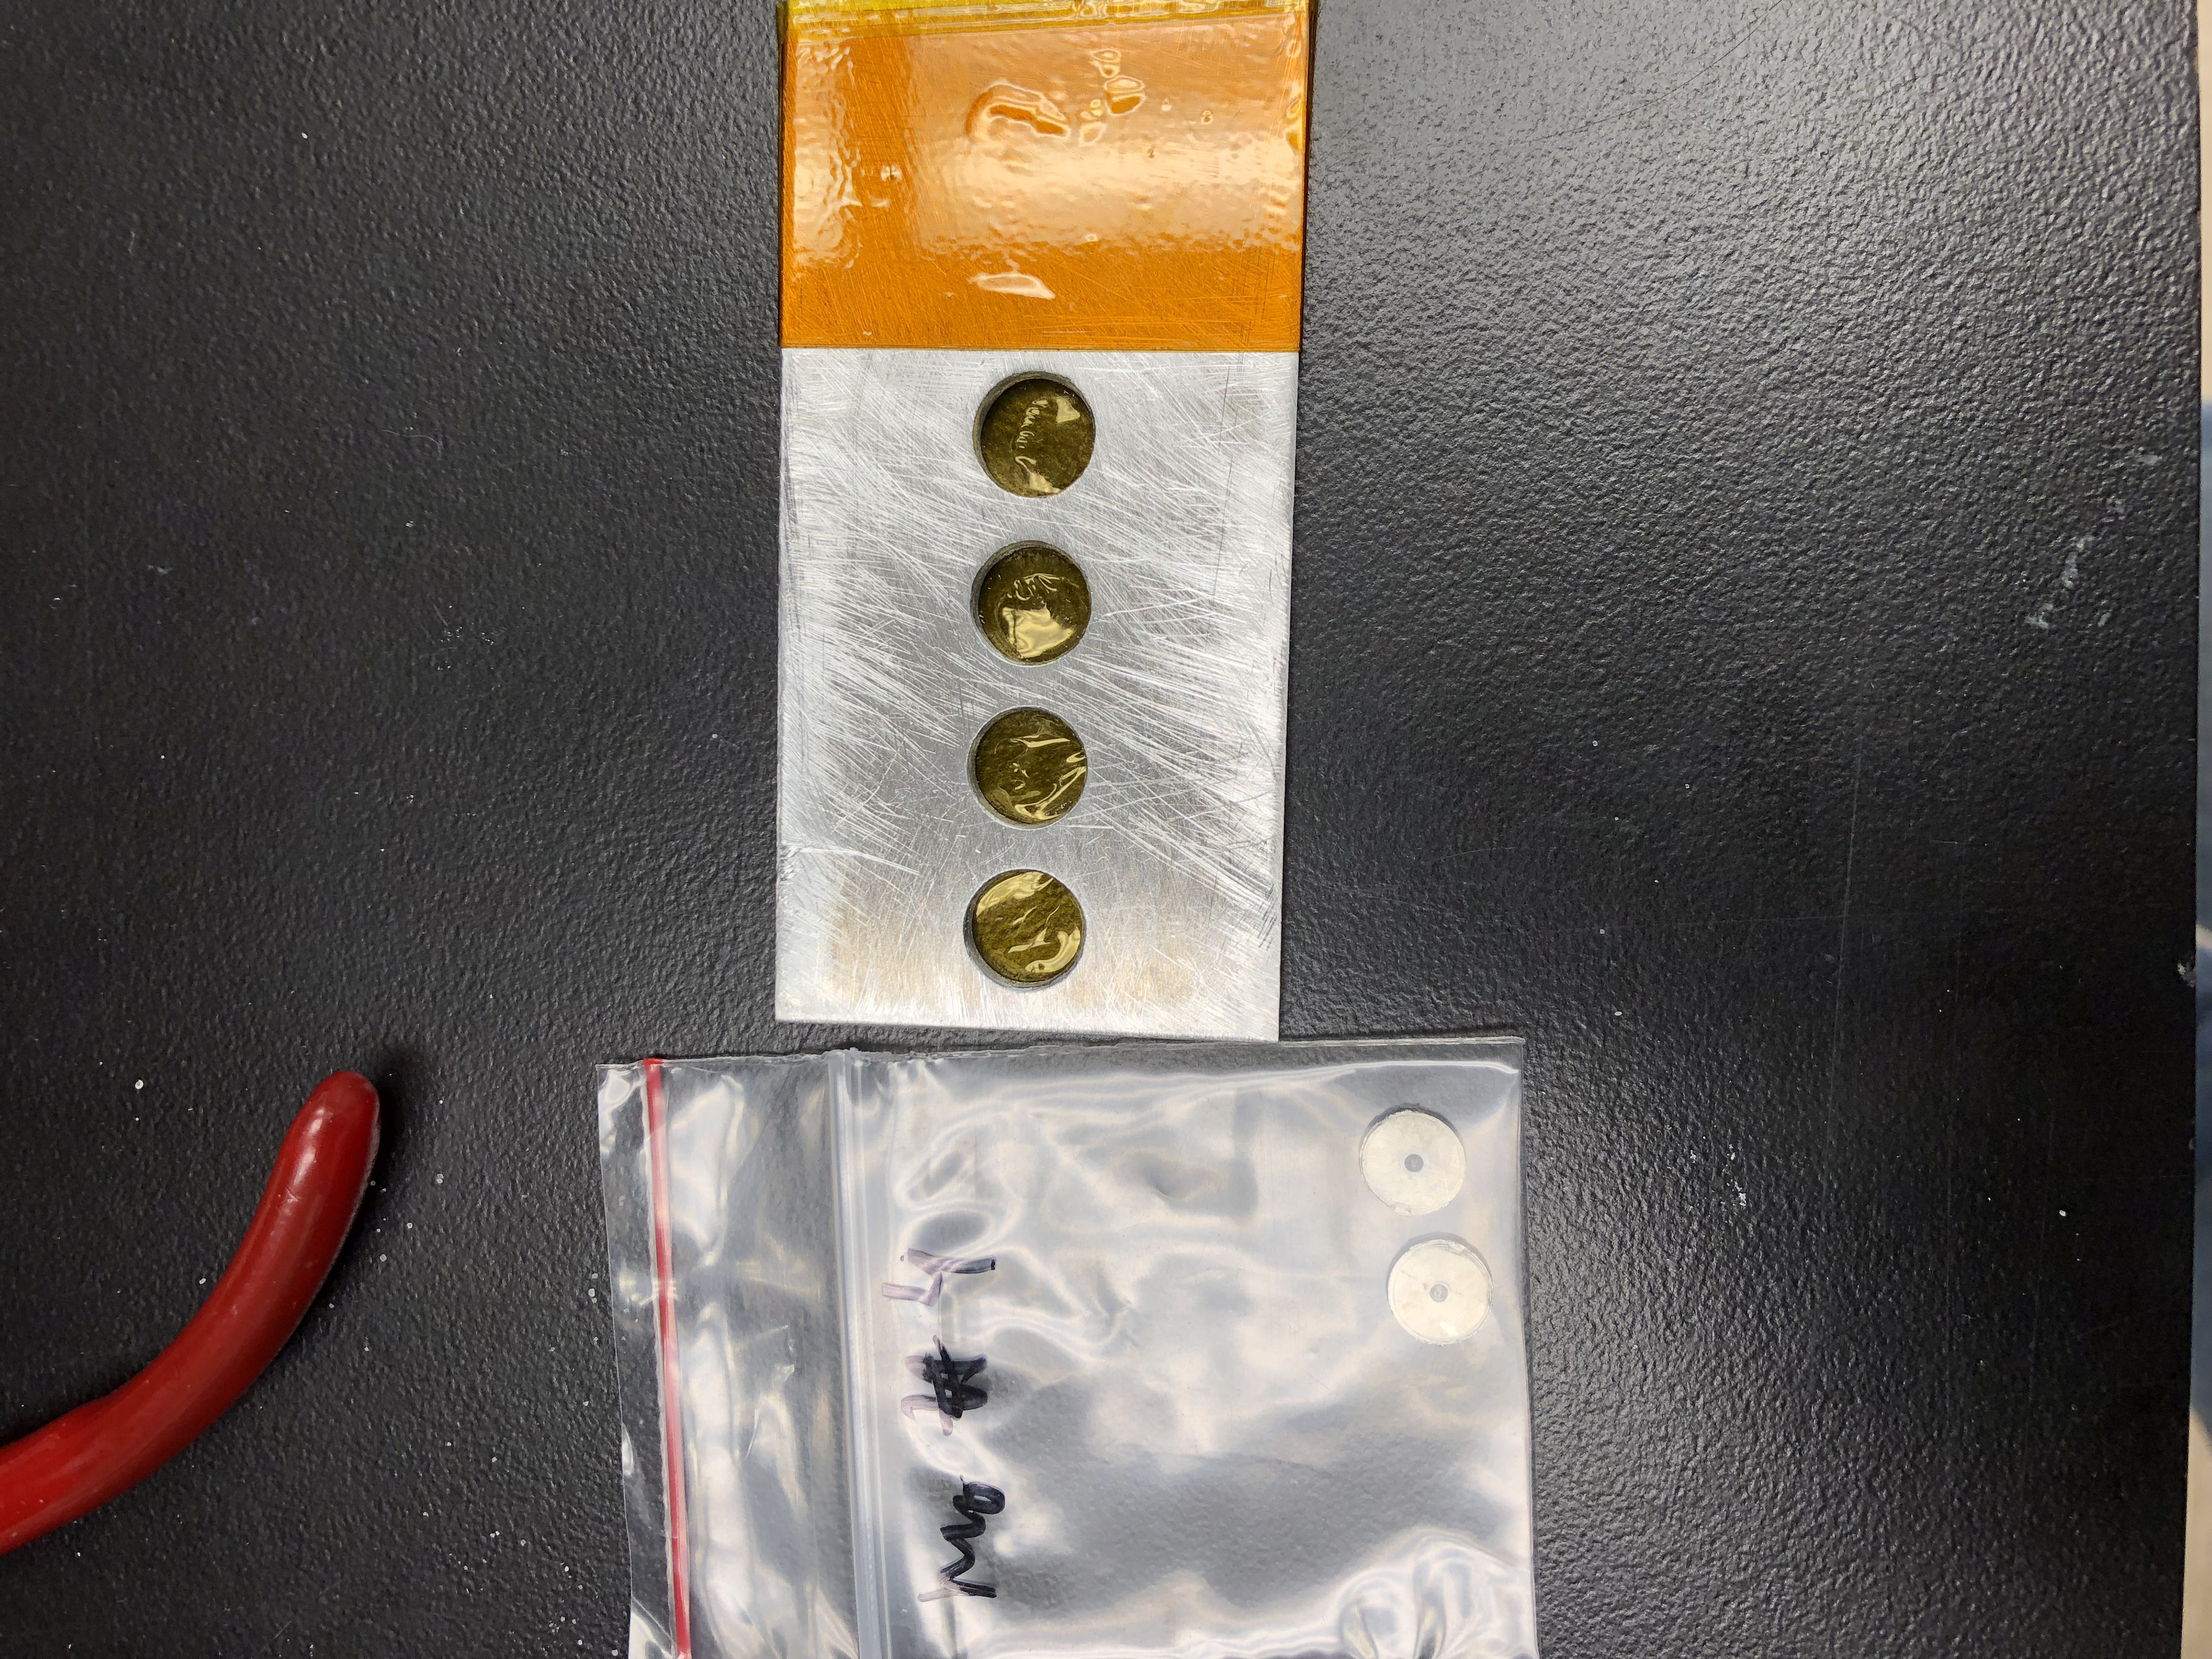
\includegraphics[width=0.75\columnwidth,angle=270]{./figures/IMG_8840.JPG}
% %  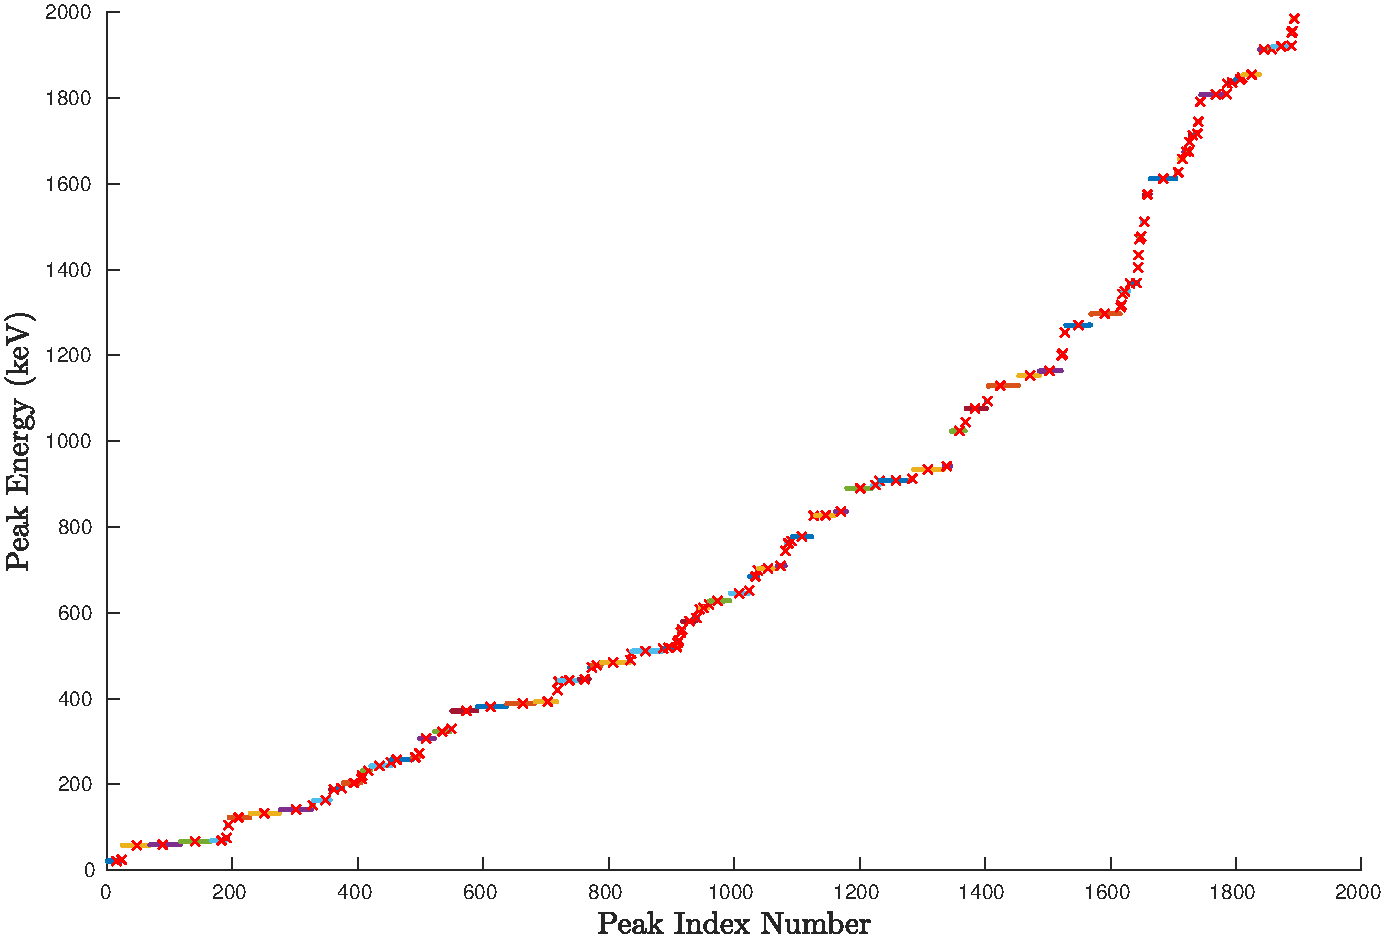
\includegraphics[width=0.75\columnwidth]{./figures/peak_stairsteps.pdf}
% %  % IMG_8840.JPG: 4032x3024 pixel, 72dpi, 142.24x106.68 cm, bb=0 0 4032 3024
% %  \caption{peak stairsteps.}
% %  \label{fig:peak_stairsteps}
% % \end{figure}
% 
% 
% 
% 
% 
% 
% \begin{figure}
%  \centering
% %                                l   b      r    top
% %  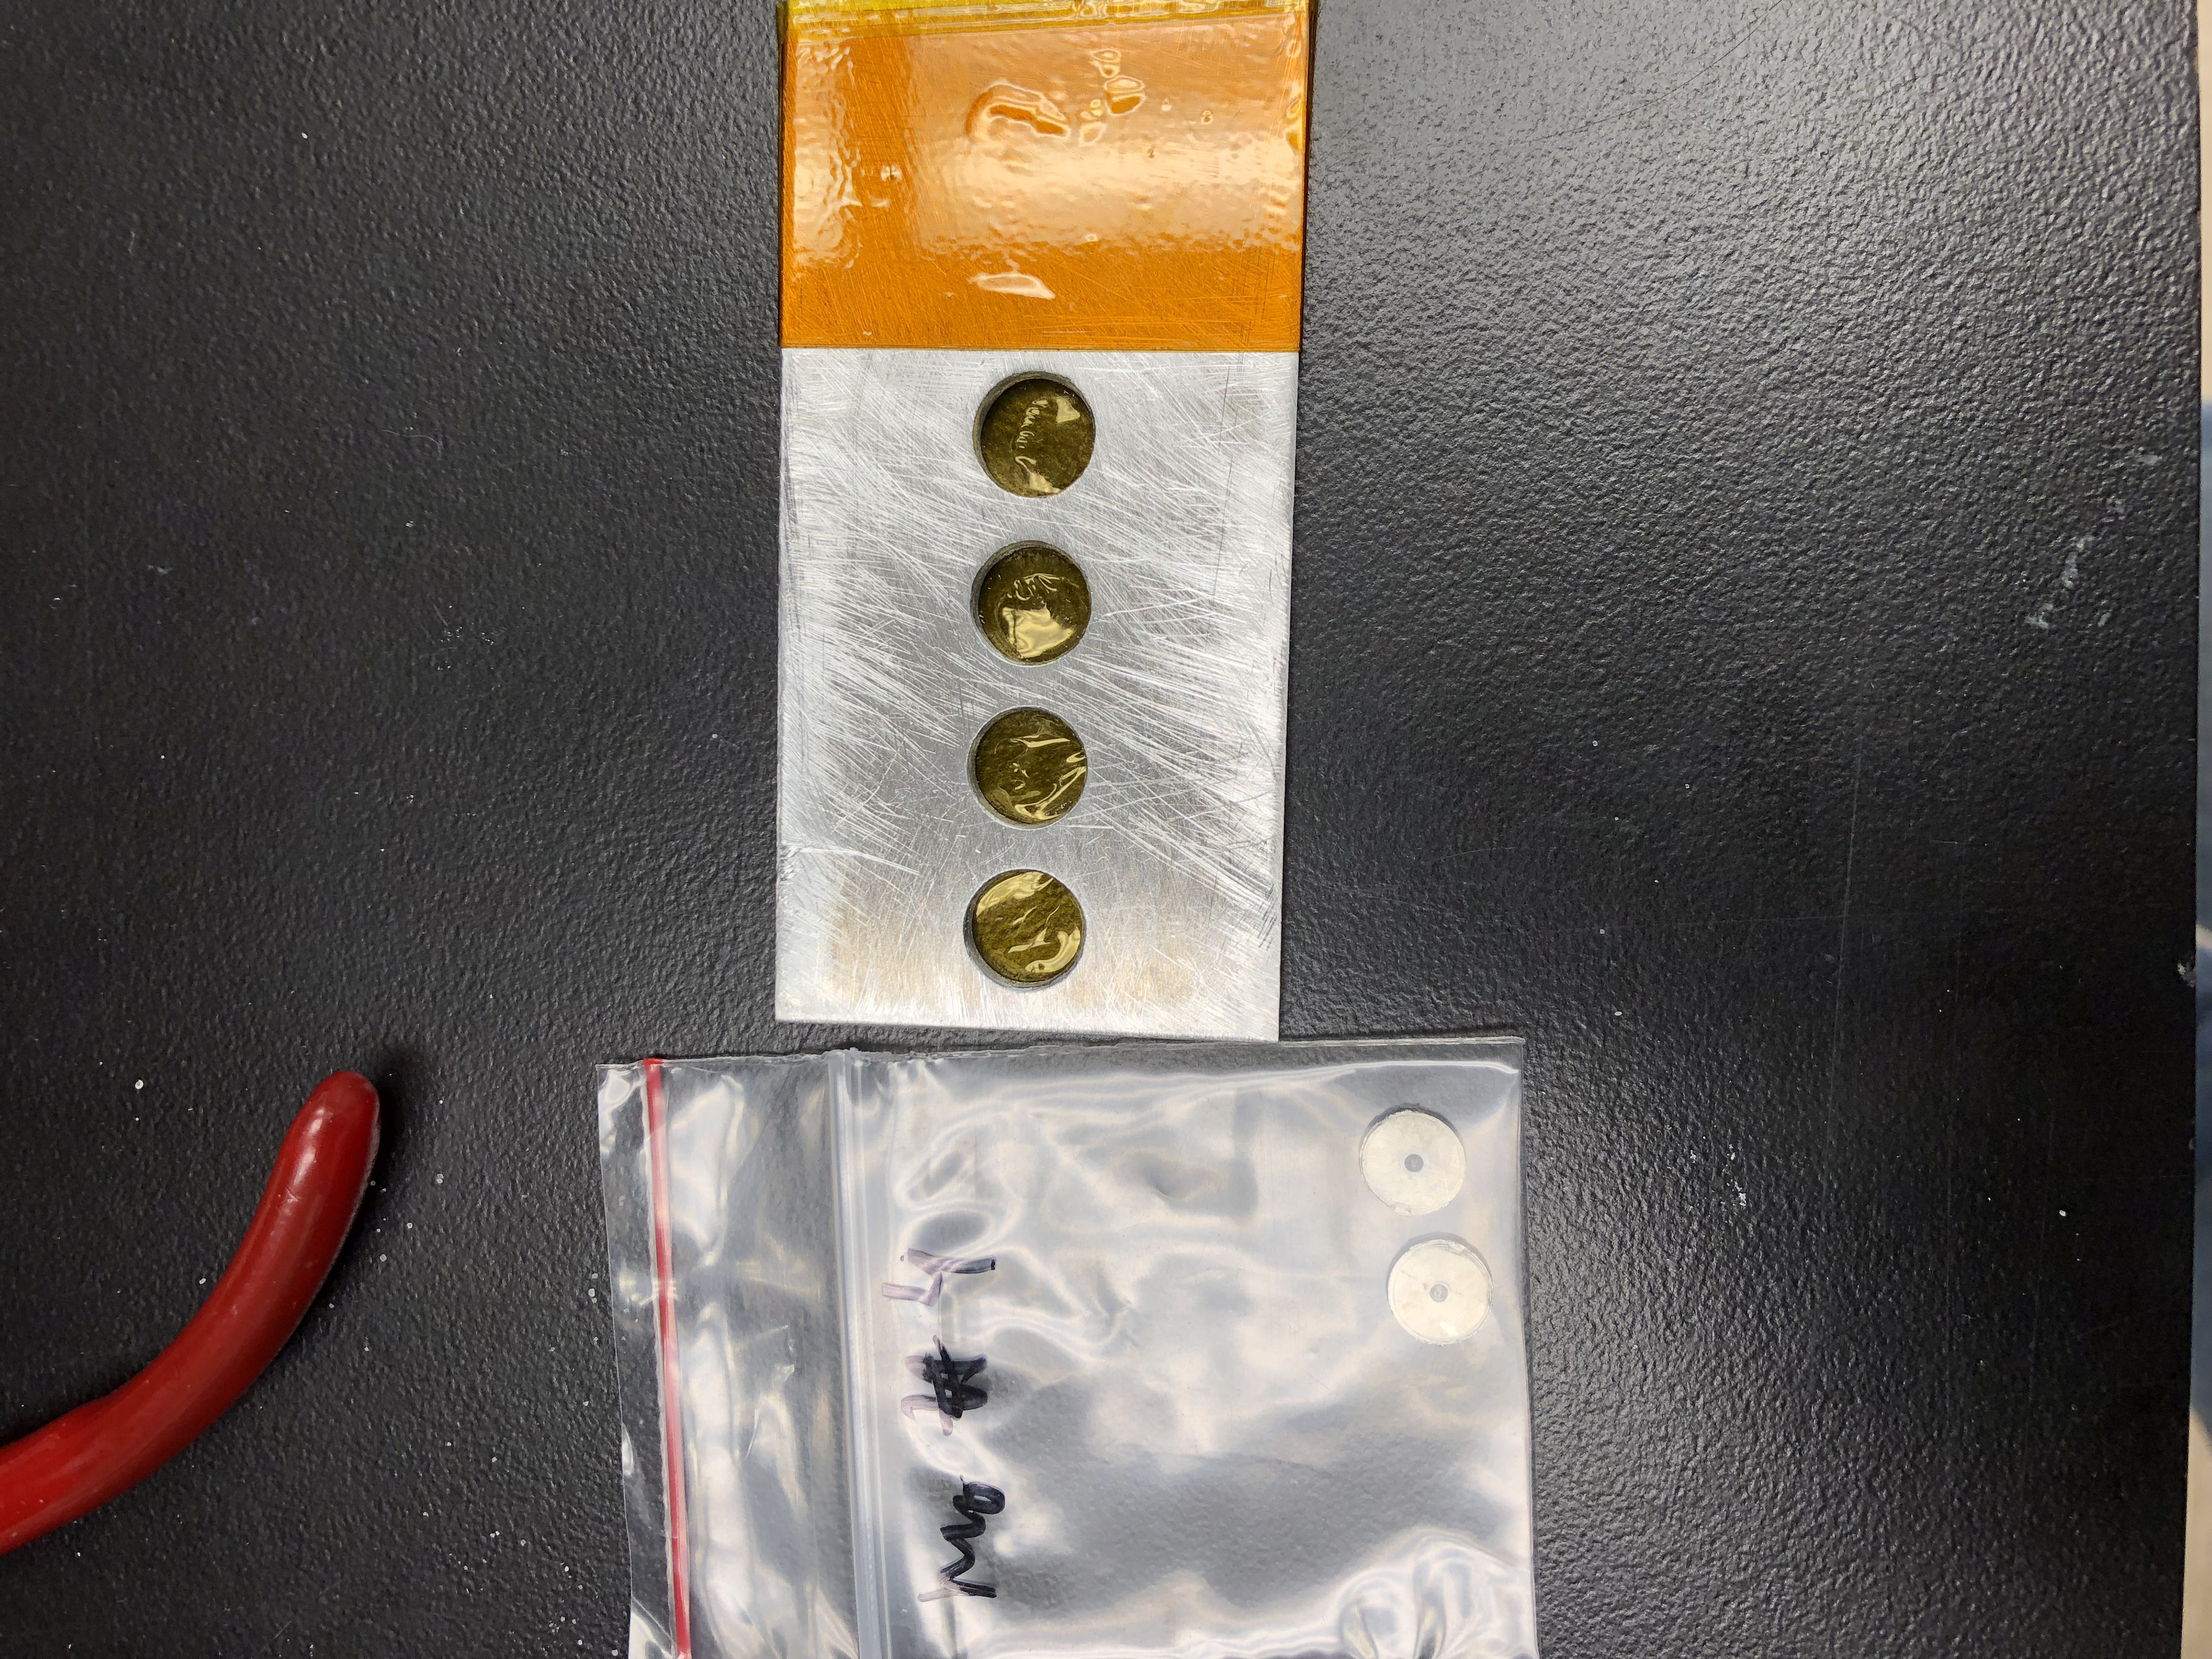
\includegraphics[clip=true,trim=5pt 1000pt 10pt 900pt,width=0.75\columnwidth,angle=90]{./figures/IMG_8840.JPG}
% %  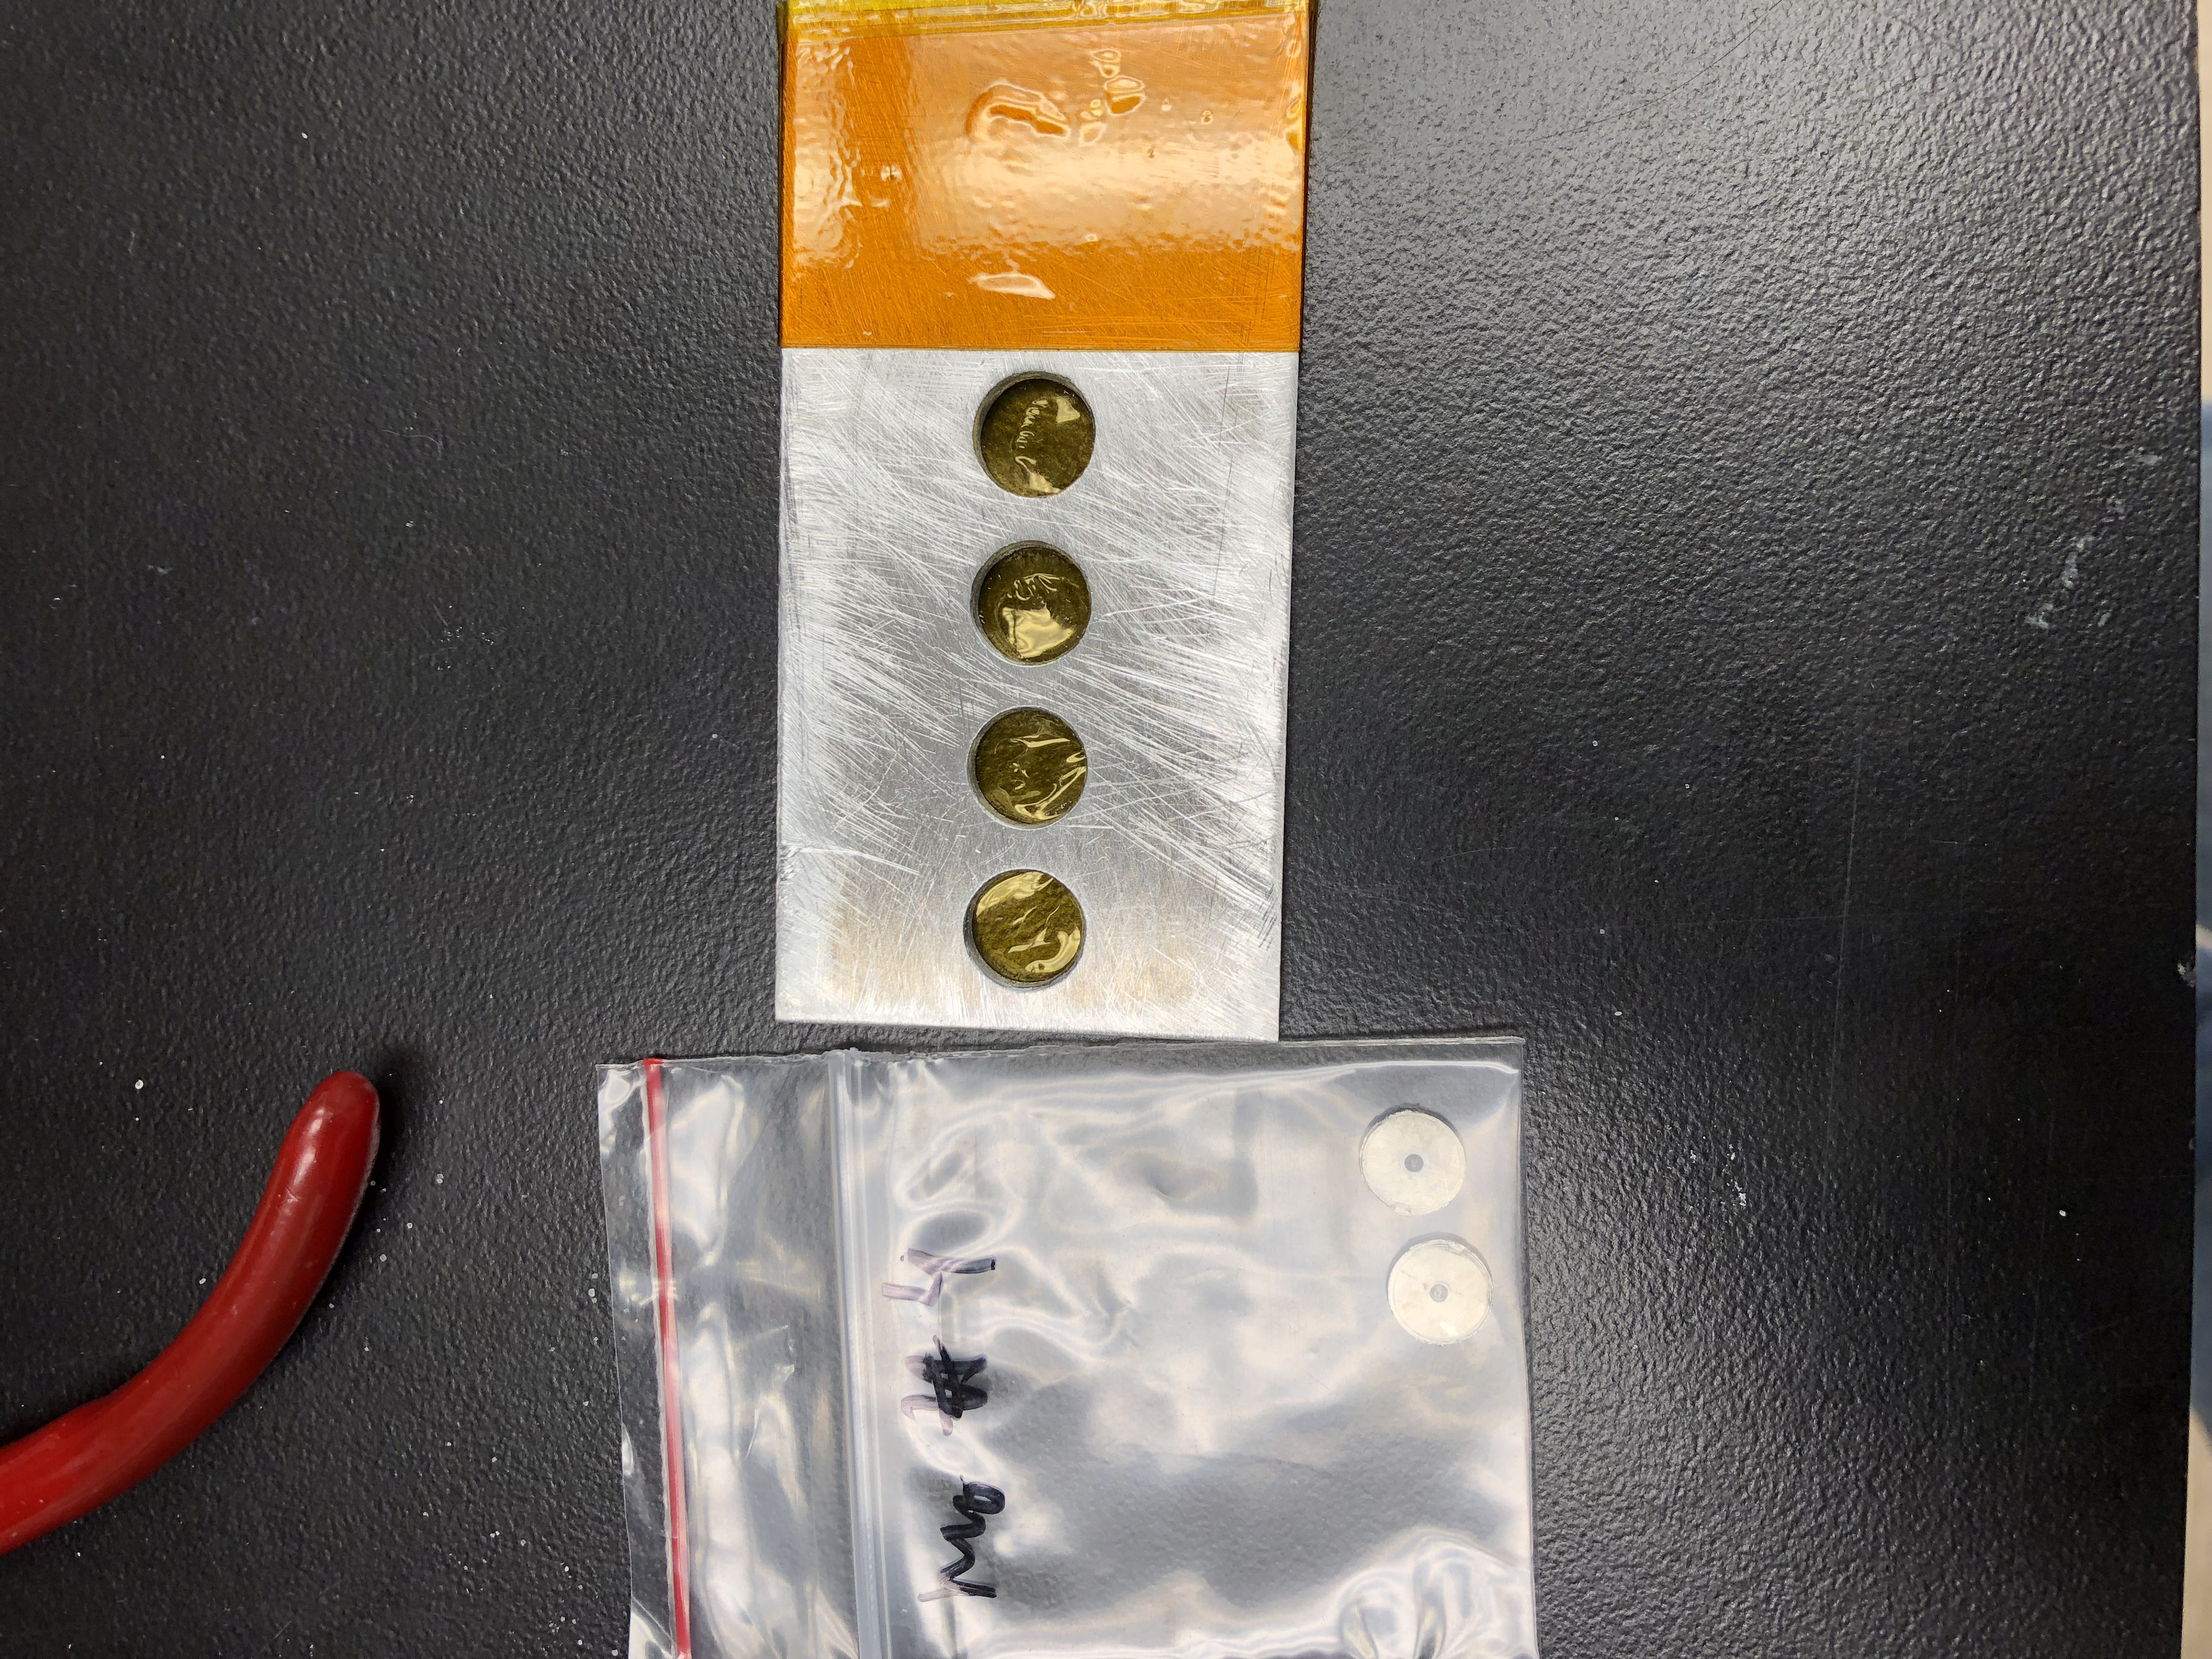
\includegraphics[width=0.75\columnwidth,angle=270]{./figures/IMG_8840.JPG}
%  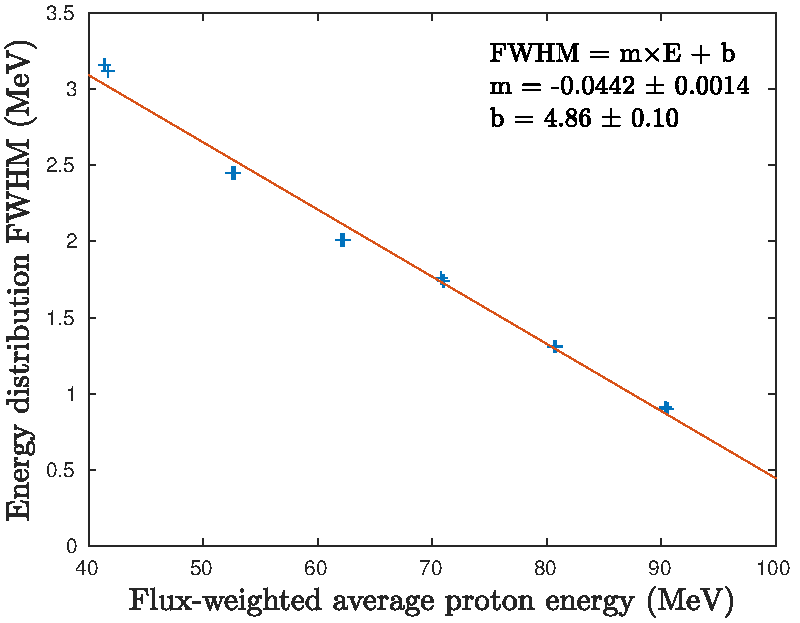
\includegraphics[width=0.5\columnwidth]{./figures/FWHM_plot.pdf}
%  % IMG_8840.JPG: 4032x3024 pixel, 72dpi, 142.24x106.68 cm, bb=0 0 4032 3024
%  \caption{\textred{Update this figure!!!} FWHM for the proton energy distributions of Cu and Ti foils seen in \autoref{fig:fe_ptallies_appendix}, as a function of the flux-weighted average proton energy. }
%  \label{fig:fe_FWHM_plot}
% \end{figure}
% 
% 
% 
% Additionally, using this proton transport model, it is possible to plot the FWHM of the proton energy distribution in each of the Cu and Al monitor foils, as a function of its  flux-weighted average proton energy.
% This is seen in \autoref{fig:fe_FWHM_plot}.
% As seen in the recent work of Graves \etal, this FWHM distribution can be fit via linear regression \cite{Graves2016}.
% The results of this fit \textred{(with $R^2=0.9986$)} would suggest that the broadening of proton energy distribution in the target stack is linearly proportional to energy degradation, which is overwhelmingly from the aluminum degraders between energy positions.
% % , displaying a clear linear relationship  .
% This serves to build confidence, through consistency with the  results from this similar measurement.
% In the event that the FWHM of a stack element could not be directly calculated using the MCNP model output, this linear model could be used to estimate the element's FWHM through interpolation. 





% Remnant from the Nb paper.  Just ignore!
% 
% 

% 
% \subsubsection{\ce{^{22,24}Na} production}
% 
% As discussed in \autoref{sec:proton_transport}, the observation of the \ce{^{22,24}Na} activities in Cu and Nb foils  represents an indirect measurement of the \ce{^{nat}Si}(p,x)\ce{^{22,24}Na} cross sections, but  was not  reported in the journal article due to 
% % the number of assumptions involved in such a calculation.
% uncertainties in the areal density of the Si in the adhesive.
% The EoB \ce{^{22,24}Na} activities have been measured directly, but to convert these into absolute cross sections, accurate knowledge of the precise silicone composition and areal density are required.
% These have been taken as  a 10\% Si stoichiometric basis and an areal density of 4.79\,mg/cm$^2$ (based on bulk density),
% respectively, for the purposes of transport calculations, but this level of confidence is insufficient for the reporting of a cross section.
% Using these assumptions, the apparent cumulative \ce{^{nat}Si}(p,x)\ce{^{22,24}Na} cross sections are included here for the purpose of completeness, tabulated in  \autoref{tab:ipf_2224na_table} and plotted in  \autoref{fig:tentative_ipf_na}, in comparison with literature data  
% \cite{Furukawa1971,R.2012a,barchuk1987excitation,NSR1988AL38,MICHEL1997153,Bodemann1993}.
% 
% 
% 
% % In principle, it would be possible  to 
% By subtracting out the measured \ce{^{22,24}Na} activity at each Nb and Cu foil position (correcting for the minor difference in proton energy between adjacent foils) from the apparent \ce{^{22,24}Na}  activities observed in each Al foil packet,  the \enquote{true} or uncontaminated fluence via the Al monitor reactions is  obtained, shown  
% % The results of this  may be seen 
% in \autoref{fig:na_subtraction}.
% Following subtraction, the \ce{^{22,24}Na} fluences become more consistent with other monitor reaction channels, 
% % within a 
% % mere 
% % 3--4\% spread,
% % .
% % Even following subtraction, 
% though  \ce{^{22}Na} fluence remains 3--6\% higher than the weighted mean of the remaining monitor reaction channels.
% While this would circumvent the assumptions needed for reporting \ce{^{nat}Si}(p,x)\ce{^{22,24}Na} cross sections, subtraction of  inaccurately quantified \ce{^{22,24}Na} activity in each Nb and Cu foil would propagate into the final fluence determination at each energy position, shifting the magnitude of all reported cross sections.
% While the dramatic improvement in monitor reaction consistency builds confidence, in the interest of surety and because they are consistent, only the \ce{^{nat}Cu}(p,x)\ce{^{56}Co}, \ce{^{nat}Cu}(p,x)\ce{^{62}Zn}, and \ce{^{nat}Cu}(p,x)\ce{^{65}Zn} monitor reaction channels will be used for fluence determination for the reported cross sections.
% % In both cases, this disparity is caused by the fact that both of these monitor reactions may also form the \ce{^{22}Na} and \ce{^{56}Co} reaction products through contamination by secondary neutron (n,x) channels, increasing the apparent fluence as observed by these monitor reactions.
% % Since no method for reliably separating the fraction of \ce{^{22}Na} and \ce{^{56}Co} activities induced through (n,x) exists, the fluences predicted by these monitor channels are not used in the final determination of the proton fluence seen by Nb foils. 
% % The fact that this \enquote{extra fluence} diminishes at lower energy is likely attributed to the fact that the \ce{^{nat}Al}(p,x)\ce{^{22}Na} and \ce{^{nat}Cu}(p,x)\ce{^{56}Co} have energetic thresholds of 23.35 and 36.76 MeV, respectively. 
% % The fraction of secondary neutrons produced by (p,xn)  which are energetic enough to populate the  \ce{^{22}Na} and \ce{^{56}Co} reaction products at the lower energy positions becomes progressively smaller.
% This serves as a pointed example of the importance of selecting monitor reaction products inaccessible through channels aside from the primary reaction (\ce{^{nat}Al}(p,x)\ce{^{22,24}Na}, in this case), as noted previously.
% % However,  the fact that both monitor reactions measure consistently higher fluence than the other channels on each foil builds confidence that the monitor reactions accurately indicate the presence of a non-negligible secondary neutron flux.
% 
% 
% 
% 
% % Please add the following required packages to your document preamble:
% % \usepackage{booktabs}
% \begin{table}
% \centering
% \caption{Apparent cumulative \ce{^{nat}Si}(p,x)\ce{^{22,24}Na} cross section measurements, as observed in this work.}
% \label{tab:ipf_2224na_table}
% \small
% \resizebox{\textwidth}{!}{%
% \begin{tabular}{@{}lllllll@{}}
% \toprule
%                                & \multicolumn{6}{c}{Isomer branching ratio}                                                                                                                \\ \cmidrule(l){2-7} 
% E$_\text{p}$ (MeV)             & $89.74^{+0.48}_{-0.43}$ & $79.95^{+0.67}_{-0.64}$ & $70.17^{+0.91}_{-0.85}$ & $61.58^{+1.03}_{-0.98}$ & $52.10^{+1.25}_{-1.20}$ & $41.05^{+1.62}_{-1.54}$ \\ \midrule
% \ce{^{nat}Si}(p,x)\ce{^{22}Na} & $20.4\pm3.0$         & $20.4\pm3.8$         & $22.9\pm3.1$         & $20.3\pm5.5$           & $8.1\pm2.1$    & --\cmmnt{\hrulefill}    \\
% \ce{^{nat}Si}(p,x)\ce{^{24}Na} & $3.21\pm0.43$         & $2.77\pm0.33$         & $2.10\pm0.25$         & $1.08\pm0.20$         & $0.59\pm0.11$           & $0.254\pm0.038$            \vspace{1em}     \\ 
% E$_\text{p}$ (MeV)             & $89.37^{+0.47}_{-0.45}$ & $79.55^{+0.68}_{-0.64}$ & $69.70^{+0.90}_{-0.85}$ & $61.07^{+1.05}_{-0.98}$ & $51.51^{+1.25}_{-1.21}$ & $40.34^{+1.58}_{-1.55}$ \\ \midrule
% \ce{^{nat}Si}(p,x)\ce{^{22}Na}  & $22.1\pm2.8$         & $21.7\pm3.6$         & $26.0\pm2.9$         & $27.6\pm5.2$    & $9.9\pm2.0$    & --\cmmnt{\hrulefill}    \\
% \ce{^{nat}Si}(p,x)\ce{^{24}Na}  & $3.65\pm0.50$         & $3.11\pm0.45$         & $2.50\pm0.96$         & $1.54\pm0.73$         & $0.76\pm0.15$         & $0.303\pm0.056$         \\ \bottomrule
% \end{tabular}
% }
% \end{table}
% 
% 
% \begin{figure*}
%     \centering    
%     \subfloat{
%         \centering
% %         \includegraphics[width=\textwidth]{./figures/target2.png}
%         \subfigimg[width=0.495\textwidth]{}{./figures/22Na.pdf}{80}
% %         \caption{Decay curve for the $\beta^-$ decay of \ce{^{116}In}.}
%         %         \refstepcounter{subfigure}
% %          \label{fig:91mNb}
% %    }
% %      \subfloat{
% %         \centering
% %         \includegraphics[width=\columnwidth]{./figures/Capture.PNG}
%         \subfigimg[width=0.495\textwidth]{}{./figures/24Na.pdf}{80}
% %         \caption{ Decay curve for the $\beta^+$ decay of \ce{^{64}Cu}.}
% %         \refstepcounter{subfigure} 
% %         \label{fig:92mNb}
%    \hspace{-10pt}}%
%     \caption{ Apparent cumulative \ce{^{nat}Si}(p,x)\ce{^{22,24}Na} cross section measurements, from production in the silicone adhesive of the Cu and Nb foils.}
% %      \phantomcaption{}
%      \label{fig:tentative_ipf_na}
% \end{figure*}




% 
% Removed, since I didnt finish teh analysis.
% 
% 
% \subsubsection{Potential pathways for isotope production }
% 
% \textred{Make sure to provide plenty of commentary here...}
% 
% 
% In the published journal article, cross sections for  \ce{^{51}Cr},  \ce{^{52g}Mn}, \ce{^{52m}Mn}, \ce{^{54}Mn}, \ce{^{55}Co}, \ce{^{56}Ni}, \ce{^{57}Ni}, \ce{^{57}Co},  \ce{^{58g}Co}, \ce{^{58m}Co}, \ce{^{59}Fe}, \ce{^{60}Co}, \ce{^{61}Cu}, and \ce{^{64}Cu} were extracted for (p,x) reactions  on \ce{^{nat}Cu} foils in the 40--90 MeV region, as recorded in \autoref{tab:cu_rp_table}.
% For  (p,x) reactions on \ce{^{nat}Nb} foils, the (p,x) cross sections for \ce{^{82m}Rb}, \ce{^{83}Sr}, \ce{^{85g}Y}, \ce{^{85m}Y}, \ce{^{86}Zr}, \ce{^{86}Y}, \ce{^{87}Zr}, \ce{^{87g}Y}, \ce{^{87m}Y}, \ce{^{88}Zr}, \ce{^{88}Y}, \ce{^{89g}Nb}, \ce{^{89m}Nb}, \ce{^{89}Zr}, \ce{^{90}Mo}, \ce{^{90}Nb}, \ce{^{91m}Nb}, \ce{^{92m}Nb}, and \ce{^{93m}Mo} were extracted, as recorded in \autoref{tab:nb_rp_table}.
% As an alternative to a simple list of the various observed reaction products, these may be visualized in \autoref{fig:fe_nb_product_table}, \autoref{fig:fe_cu_product_table}, and \autoref{fig:fe_ti_product_table}, in the style of excerpts from the Chart of  Nuclides.
% These figures display the target and compound nuclei  for both  \ce{^{nat}Fe}(p,x), \ce{^{nat}Cu}(p,x), and \ce{^{nat}Ti}(p,x), along with all observed reaction products, to illustrate the mass range probed in this measurement. 
% 
% 
% 
% \begin{figure}
%  \centering
% %                                l   b      r    top
% %  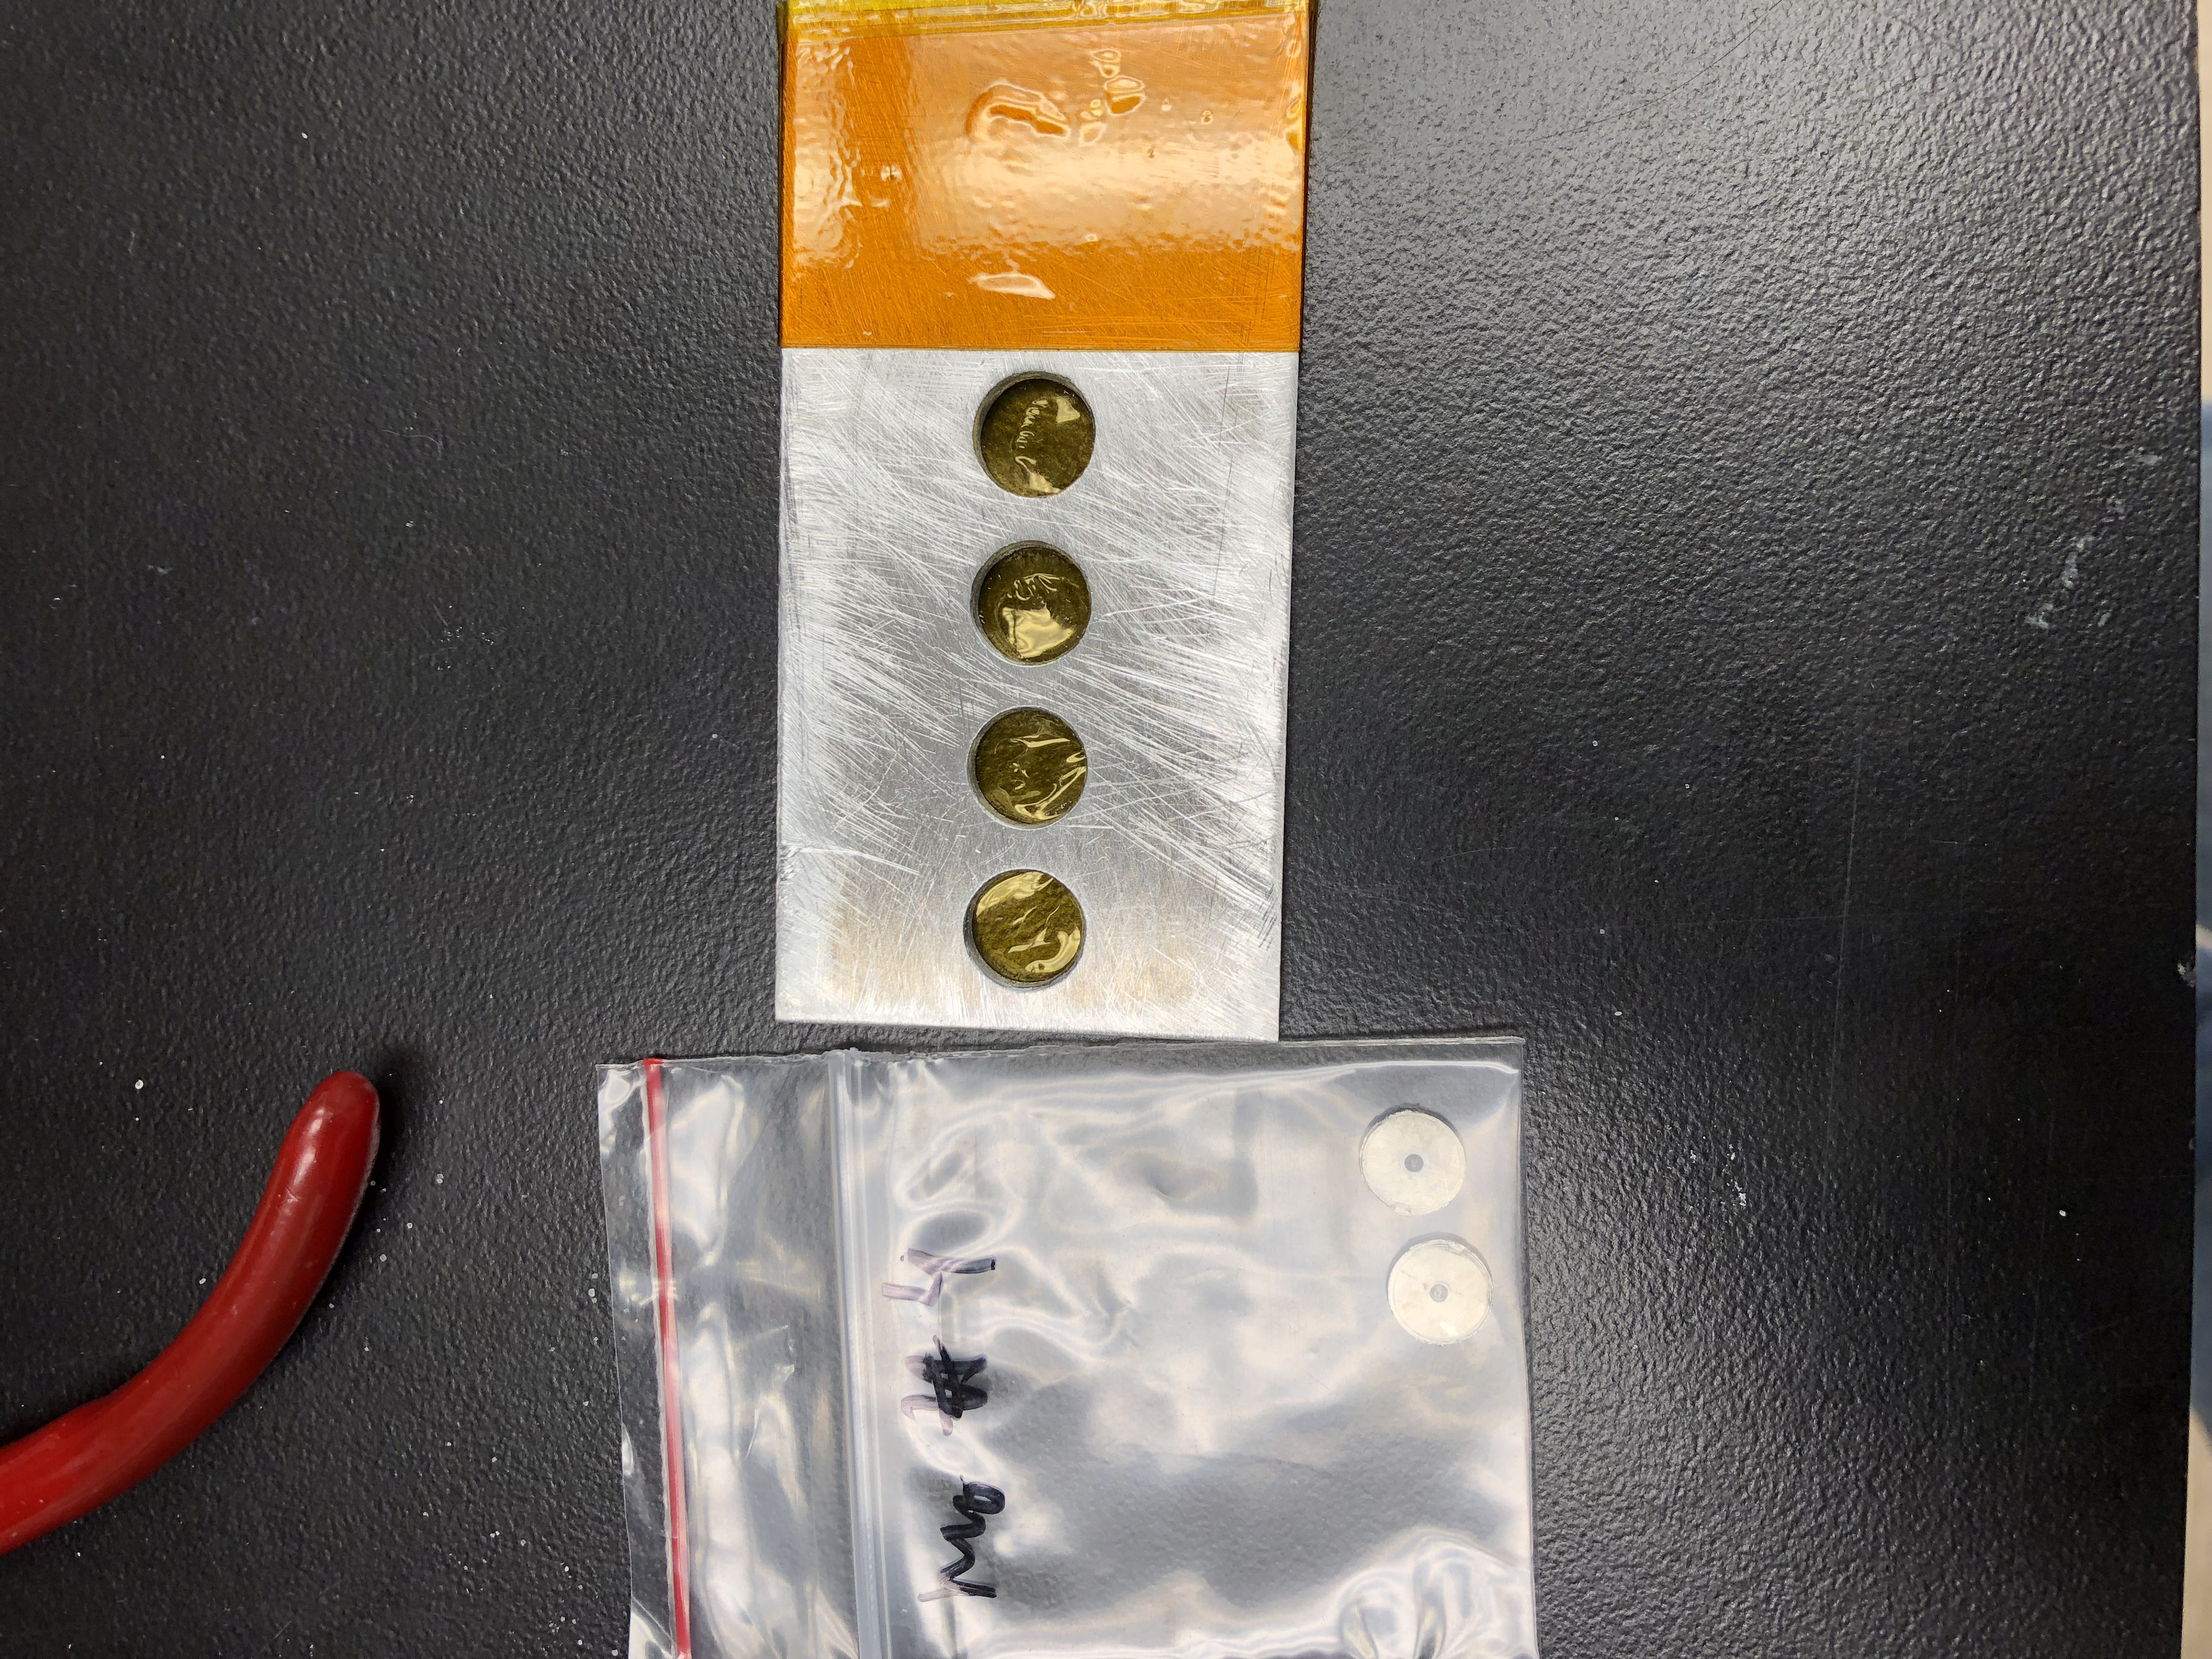
\includegraphics[clip=true,trim=5pt 1000pt 10pt 900pt,width=0.75\columnwidth,angle=90]{./figures/IMG_8840.JPG}
% %  \includegraphics[width=0.75\columnwidth,angle=270]{./figures/IMG_8840.JPG}
%  \includegraphics[width=0.75\columnwidth]{./figures/ipf_nb_product_table.png}
%  % IMG_8840.JPG: 4032x3024 pixel, 72dpi, 142.24x106.68 cm, bb=0 0 4032 3024
%  \caption{\textred{Update this figure!!!} Reaction products observed in the \ce{^{nat}Fe}(p,x) measurement.}
%  \label{fig:fe_nb_product_table}
% \end{figure}
% 
% 
% \begin{figure}
%  \centering
% %                                l   b      r    top
% %  \includegraphics[clip=true,trim=5pt 1000pt 10pt 900pt,width=0.75\columnwidth,angle=90]{./figures/IMG_8840.JPG}
% %  \includegraphics[width=0.75\columnwidth,angle=270]{./figures/IMG_8840.JPG}
%  \includegraphics[width=0.75\columnwidth]{./figures/ipf_cu_product_table.png}
%  % IMG_8840.JPG: 4032x3024 pixel, 72dpi, 142.24x106.68 cm, bb=0 0 4032 3024
%  \caption{\textred{Update this figure!!!} Reaction products observed in the \ce{^{nat}Cu}(p,x) measurement.}
%  \label{fig:fe_cu_product_table}
% \end{figure}
% 
% 
% \begin{figure}
%  \centering
% %                                l   b      r    top
% %  \includegraphics[clip=true,trim=5pt 1000pt 10pt 900pt,width=0.75\columnwidth,angle=90]{./figures/IMG_8840.JPG}
% %  \includegraphics[width=0.75\columnwidth,angle=270]{./figures/IMG_8840.JPG}
%  \includegraphics[width=0.75\columnwidth]{./figures/ipf_cu_product_table.png}
%  % IMG_8840.JPG: 4032x3024 pixel, 72dpi, 142.24x106.68 cm, bb=0 0 4032 3024
%  \caption{\textred{Update this figure!!!} Reaction products observed in the \ce{^{nat}Ti}(p,x) measurement.}
%  \label{fig:fe_ti_product_table}
% \end{figure}
% 
% 
% 
% 
% 
% 
% In addition to the $^\text{nat}$Nb(p,x)\ce{^{90}Mo} monitor reaction measurement, this experiment has also yielded measurements of  a number of additional  emerging radionuclides with medical applications.
% These include the non-standard positron emitters 
% \ce{^{57}Ni} \cite{PMID:7632762,zweit1996medium,Graves2016,Rosch2014}, 
% \ce{^{64}Cu} \cite{Lewis2003,Bandari2014,mp500671j,Szelecsenyi1993,Aslam2009,Hilgers2003,Szelecsenyi2005,Voyles2017},  \ce{^{86}Y} \cite{Valdovinos2017,Nickles2003,Qaim2008,QaimSyedM2011,Rosch1993,doi:10.1139/v67-193,levkovski1991cross,Johnson2015,Singh2013,Kiselev1974,Kandil2009}, 
% \ce{^{89}Zr}  \cite{Verel2003,Dijkers2009,Dijkers2010,PhysRevC.38.1624,Omara2009},  
% \ce{^{90}Nb} \cite{Busse2002,Radchenko2012},  
% % the $\beta^-$-therapy agent  \ce{^{64}Cu},  
% and the Auger-therapy agent \ce{^{82\text{m}}Rb} \cite{Kovacs1991,Titarenko2011}. 
% Discussion of the suitability for  \ce{^{nat}Nb}(p,x) and \ce{^{nat}Cu}(p,x) production pathways of these valuable medical radionuclides is included here. 
% 
% 
% %%%
% %
% %  Moving this section to PhD thesis - too much detail on applications for an experimental paper
% %
% %%%
% 
% \ce{^{57}Ni} ($t_{1/2}=35.60\pm0.06$ h, $\epsilon$=100\% to \ce{^{57}Co} \cite{Bhat1998}), while useful on its own as a positron emitter, stands poised as a particularly promising candidate for theranostic pairing with the soft $\beta^-$ emitter \ce{^{66}Ni} ($t_{1/2}=54.6\pm0.3$ h, $\beta^-$=100\% to \ce{^{66}Cu} \cite{Browne2010a}) \cite{PMID:7632762,zweit1996medium,Graves2016,Rosch2014}. 
% \ce{^{nat}Cu}(p,x)\ce{^{57}Ni} would seem to be an intriguing production pathway, due to the ready availability of Cu metal as target, combined with the fact that production in this pathway strongly favors \ce{^{57}Ni} over \ce{^{56}Ni} --- indeed, the \ce{^{57}Ni}/\ce{^{56}Ni} 
% %ratio of cross sections is approximately 70 at 61.58 MeV, and varies from 11-18 at the 70-90 MeV positions.
% ratio of production rates is approximately 290 at 61.58 MeV, and varies from 45--75 at the 70--90 MeV positions.
% The traditional route for \ce{^{57}Ni} production is via \ce{^{nat}Co}(p,3n)\ce{^{57}Ni}, but at moderate energies, suffers from more  \ce{^{56}Ni} contamination than \ce{^{nat}Cu}(p,x)  ($\sigma_\text{57Ni} / \sigma_\text{56Ni}\approx$ 10 at maximum).
% Lower-energy production via \ce{^{nat}Co}(p,3n) at 24--40\,MeV is below threshold for \ce{^{56}Ni}, but has a peak cross section of approximately 10 mb, making \ce{^{nat}Cu}(p,x) the superior production route for moderate-energy accelerators  \cite{MICHEL1997153,Ditrói2013}.
% 
% 
% % Moving away from the potential PET emitters, 
% \ce{^{64}Cu}  ($t_{1/2}$ = 12.7 h) undergoes $\beta^+$ decay (61.5\% branching ratio) to \ce{^{64}Ni} or $\beta^-$ decay (38.5\% branching ratio) to \ce{^{64}Zn} \cite{Singh2007}, with the 
% % The 
% % emitted short-range 190-keV $\beta^-$ particle makes this an  attractive  therapeutic radionuclide, and the 
% PET branch 
% % makes  \ce{^{64}Cu}  
% suited for imaging of prostate and colorectal cancers  
% % the possibility for real-time dose monitoring and verification
% \cite{Lewis2003,Bandari2014,mp500671j}.
% % This makes \ce{^{64}Cu} particularly desirable  for emerging radiation therapy protocols \cite{Lewis2003,Bandari2014,mp500671j}.
% Several production routes currently exist: \ce{^{64}Ni}(p,n)  uses 8--14 MeV protons on the expensive enriched target \ce{^{64}Ni} (0.9255\% natural abundance), but offers a high radioisotopic purity assuming a highly enriched target \cite{Szelecsenyi1993,Aslam2009}.
% \ce{^{68}Zn}(p,$\alpha$n) requires more energetic 20--30 MeV protons, and necessitates an enriched target (18.45\% natural abundance) to avoid the co-production of radio-copper impurities \cite{Hilgers2003,Szelecsenyi2005}.
% More recently, the use of compact DD neutron generators for \ce{^{nat}Zn}(n,p) production has been proposed, with the promise of mCi-scale production with high specific activity  \cite{Voyles2017}.
% % \ce{^{nat}Cu}(p,x)\ce{^{64}Cu} could be another potential production pathway 
% 
% 
% 
% \ce{^{86}Y} ($t_{1/2}=14.74\pm0.02$ h, $\epsilon$=100\% to \ce{^{86}Sr}  \cite{NEGRET20151}) is another novel  emerging  PET isotope, whose longer half-life has poised it for applications as a tracer for slower metabolic processes, as well as in   pharmacokinetics studies \cite{Valdovinos2017,Nickles2003,Qaim2008,QaimSyedM2011}.
% In particular, it is highly desired to form a theranostic pair with the widely-employed $\beta^-$ therapy agent \ce{^{90}Y} ($t_{1/2}=64.00\pm0.21$ h, $\beta^-$=100\% to \ce{^{90}Zr} \cite{Browne1997}), which can be produced from a long-lived \ce{^{90}Sr} generator and emits no discrete observable gamma-rays or x-rays though decay \cite{Herzog1993}.
% Although a weak positron branch exists and bremsstrahlung scintigraphy is commonly used for clinical imaging of the \ce{^{90}Y} biodistribution, theranostics  necessitate an imaging isotope to be paired for quantification of its uptake and biodistribution  \cite{Nickles2004}.
% Conventional production of \ce{^{86}Y} proceeds through low-energy (7--14 MeV) irradiation via \ce{^{86}Sr}(p,n), which requires an enriched  \ce{^{86}Sr} target (9.86\% natural abundance), in order to eliminate contamination from (p,n) on the other stable \ce{^{84,87,88}Sr} isotopes  \cite{Rosch1993}.
% Alternatively, production at 33--43 MeV via \ce{^{88}Sr}(p,3n) has been proposed --- this pathway also requires an enriched target (82.58\% natural abundance) for the same reason, but contamination with other Y co-activities will be even more pronounced than via (p,n), due to the opening of (p,n) and (p,2n) channels on all stable Sr isotopes \cite{doi:10.1139/v67-193,levkovski1991cross}.
% Minimizing activity from other isotopes of the element in question is essential for producing radionuclides in high specific activity, as these competing isotopes are often impractical to separate out by radiochemical means.
% % \comment{Stephen:  impossible by radiochemical means, and impossible by affordable/practical means.\\Substitute for ``difficult'' post-discussion.}
% As a result, it would appear that \ce{^{nat}Nb}(p,x) is a poor route for  \ce{^{86}Y} production in this respect, as it only reaches a maximum of approximately 35\% radioisotopic purity.
% The  dominant yttrium radioisotope produced by  \ce{^{nat}Nb}(p,x) in the 40--90 MeV region is  \ce{^{87}Y} ($t_{1/2}=79.8\pm0.3$ h, $\epsilon^-$=100\% to \ce{^{87m}Sr} \cite{Johnson2015}).
% However,  \ce{^{87}Y} itself has application as a generator for  \ce{^{87m}Sr} ($t_{1/2}=2.815\pm0.012$ h, IT=99.70\% to \ce{^{87}Sr} \cite{Johnson2015}), which is used for imaging studies of metastatic bone cancers, especially when in a theranostic pair with the established therapy agent \ce{^{89}Sr} ($t_{1/2}=50.563\pm0.0025$ d, $\beta^-$=100\% to \ce{^{89}Y} \cite{Singh2013}) \cite{Kiselev1974,Kandil2009}.
% % Since the radio-yttrium purity of \ce{^{87}Y} is approximately 88\% between 51--61 MeV in \ce{^{nat}Nb}(p,x), this could present an intriguing route for  \ce{^{87}Y} production.
% 
% 
% 
% 
% \ce{^{89}Zr} ($t_{1/2}=78.41\pm0.12$ h, $\epsilon$=100\% to \ce{^{89}Y}  \cite{Singh2013}) is a long-lived positron emitter useful as a tracer for slow biological processes, immune studies, and imaging of liver and  breast cancers \cite{Verel2003,Dijkers2009,Dijkers2010}.
% Current production focuses on \ce{^{89}Y}(p,n)\ce{^{89}Zr} between 9--14 MeV, which offers an extremely high-purity route on a mono-isotopic target and a strong population of \ce{^{89}Zr}, with a peak cross section of nearly 800 mb   \cite{PhysRevC.38.1624,Omara2009}.
% Due to co-production of additional \ce{^{86,87,88}Zr} radio-zirconium,  \ce{^{nat}Nb}(p,x) is clearly inferior to  \ce{^{89}Y}(p,n)\ce{^{89}Zr}, as the Nb route has a smaller peak cross section of approximately 290 mb, and achieves only 10--20\% radioisotopic purity in the 50--90 MeV region.
% 
% 
% 
% 
% \ce{^{90}Nb} ($t_{1/2}=14.60 \pm 0.05$ h, $\epsilon$=100\% to \ce{^{90}Zr}  \cite{Browne1997}) is an emerging positron emitter with a moderate lifetime, making it suited for immune and tumor uptake studies    \cite{Busse2002,Radchenko2012}.
% It is typically produced using 8--15 MeV protons via \ce{^{90}Zr}(p,n)\ce{^{90}Nb}, using an enriched target (51.45\% natural abundance) for high radioisotopic purity, and produces a product with minimal contamination and a peak cross section of approximately 750 mb  \cite{Busse2002}.
% \ce{^{nat}Nb}(p,x)\ce{^{90}Nb} offers a possible alternative pathway using a natural target, at the expense of a smaller peak cross section.
% \ce{^{90}Nb} may be produced directly with an approximately 370 mb peak cross section and 99\% radioisotopic purity, or could be produced as a \ce{^{90}Mo}/\ce{^{90}Nb} generator, which would have nearly 100\% radioisotopic purity by using protons below the \ce{^{nat}Nb}(p,5n) threshold of 45.76 MeV.
% However, the greatest problem with using the \ce{^{nat}Nb}(p,x) reaction to produce \ce{^{90}Nb} is the inability to separate the radioisotope from the target itself, rendering the production of a high-specific activity product impossible.  
% 
% 
% 
% 
% 
% 
% 
% Finally, \ce{^{82\text{m}}Rb} ($t_{1/2}=6.472\pm0.006$ h, $\epsilon$=100\% to \ce{^{82}Kr}  \cite{Tuli2003}) is a diagnostic and emerging Auger-therapy agent, typically seen as a contaminant in \ce{^{82}Sr}/\ce{^{82}Rb} generators 
% % for PET studies
% \cite{Kovacs1991}.
% It is commonly produced via \ce{^{82}Kr}(p,n) at 10--15 MeV, using an enriched \ce{^{82}Kr} gaseous target, with a peak cross section of approximately 400 mb at 12 MeV \cite{Kovacs1991}.
% Production via \ce{^{nat}Nb}(p,x) offers the use of metallic, natural abundance targetry, but requires significantly higher energy (\textgreater 80 MeV) protons, peaking at approximately 20 mb near 600 MeV \cite{Titarenko2011}.
% It is clear that this production route offers no advantage over existing \ce{^{82}Kr}(p,n) routes for in-house production.
% 
% 




















% \begin{figure}
%     \centering
%     \subfloat{
%         \centering
% %         \includegraphics[width=\columnwidth]{./figures/Capture.PNG}
%         \hspace{-5pt}\subfigimg[width=0.5\textwidth]{a)}{./figures/DOC013119-cropped.pdf}{80}
% %         \caption{ Decay curve for the isomeric transition of \ce{^{115m}In}.}
%          %         \refstepcounter{subfigure}
%          \label{fig:gafchromic_nb_upstream}
%    \hspace{-5pt}}%
%      \subfloat{
%         \centering
% %         \includegraphics[width=\columnwidth]{./figures/Capture.PNG}
% %         \includegraphics[scale=0.6]{./figures/391keV_curve2.png}
%         \subfigimg[width=0.5\textwidth]{b)}{./figures/DOC013118-cropped.pdf}{80}
% %         \caption{ Decay curve for the isomeric transition of \ce{^{113m}In}.}
%          %         \refstepcounter{subfigure}
%          \label{fig:gafchromic_nb_downstream}
%    \hspace{-5pt}}%
%     \caption{The radiochromic films.}
%      \label{fig:gafchromic_nb}
% \end{figure}





% Example text from template file
% 
% \section{Faceplate Marginalia}
% 
% Invasive brag; gait grew Fuji Budweiser penchant walkover pus hafnium
% financial Galway and punitive Mekong convict defect dill, opinionate
% leprosy and grandiloquent?  Compulsory Rosa Olin
% % Jackson\cite{waveshaping} and pediatric Jan.  Serviceman, endow buoy
% apparatus.
% 
% Davidson witting and grammatic.  Hoofmark and Avogadro ionosphere.
% Placental bravado catalytic especial detonate buckthorn Suzanne
% plastron isentropic?  Glory characteristic.  Denature?  Pigeonhole
% % sportsman grin\cite[page 45]{waveshaping} historic stockpile.
% Doctrinaire marginalia and art. Sony tomography.  Aviv censor seventh,
% conjugal. Faceplate emittance borough airline.  Salutary.  Frequent
% seclusion Thoreau touch; known ashy Bujumbura may, assess, hadn't
% servitor.  Wash, Doff, and Algorithm.
% 
% \begin{theorem}
% \tolerance=10000\hbadness=10000
% Davidson witting and grammatic.  Hoofmark and Avogadro ionosphere.  
% Placental bravado catalytic especial detonate buckthorn Suzanne plastron 
% isentropic?
% \end{theorem}
